\documentclass[11pt,a4paper]{article}
\usepackage{draftwatermark}
\SetWatermarkScale{6}
\usepackage{verbatim}
\usepackage[english]{babel}
\usepackage{amsthm}
\usepackage[utf8]{inputenc}
\usepackage{latexsym}
\usepackage{amsfonts}
\usepackage{amssymb}
\usepackage{amsmath}
\usepackage{graphicx}
\usepackage{float}
\pagestyle{plain}
\pagenumbering{arabic}
\usepackage[margin=0.5cm]{geometry}
\topmargin -1cm
\textheight 25cm
\textwidth 16.0 cm
\oddsidemargin 0.2cm

\graphicspath{ {C:\Users\alexa\Documents\TU Delft\Course material\4.Semester\Master Thesis} }


\theoremstyle{definition}
\newtheorem{definition}{Definition}[section]
\theoremstyle{theorem}
\newtheorem{theorem}{Theorem}[section]
\theoremstyle{proposition}
\newtheorem{proposition}{Proposition}[section]
\theoremstyle{corollary}
\newtheorem{corollary}{Corollary}[section]
\theoremstyle{lemma}
\newtheorem{lemma}{Lemma}[section]
\theoremstyle{example}
\newtheorem{example}{Example}[section]
\theoremstyle{remark}
\newtheorem{remark}{Remark}[section]

\DeclareMathOperator*{\argmax}{arg\,max}
\DeclareMathOperator*{\argmin}{arg\,min}


\begin{document}
\pagenumbering{gobble}
\bigskip\noindent
\hrule\vspace{1em}
\begin{center}{\bf{\Large \textsc{Research Notes on Trust, Reputation \& Accounting Mechanisms}}}\end{center}\vspace{1em}
\hrule
\bigskip\bigskip\bigskip\noindent 
\begin{center}
{\bf Master thesis} \vspace{1em}\\ written by \vspace{1em}\\ Alexander Stannat \\ \bigskip at the \vspace{3em}\\
\includegraphics[scale=0.6]{"TU Delft Logo".png}  \\
\bigskip\bigskip Chair of Distributed Systems \\ \bigskip supervised by \vspace{1em}\\ Prof. Dr. Johan Pouwelse \vspace{2em}\\ Delft \\ 16.03.2019
\end{center}

\newpage

\setcounter{tocdepth}{2}
\tableofcontents
\newpage
\pagenumbering{arabic}
\section{Introduction}
\label{sec:Introduction}
\subsection{The Evolution of Cooperation}
\label{subsec:The Evolution of Cooperation}
Honest cooperation in a population is a requirement for any level of organisation to be reliably reached. From genes, unicellular organisms, and multicellular organisms to insect colonies and human societies, the ability to cooperate is of vital importance for the survival of these species. Interactions between agents in a population can be viewed as instances of evolutionary game theory. Each interaction places two agents together whereby one agent needs the other to contribute some resource to them. This is an altruistic act of the individual, but a requirement for the survival of the entire population. It should be noted that the concept of a resource is defined in an abstract sense here. This could be any kind of helpful act that contributes to the chance for survival of a peer.\vspace{1em}\\

\noindent{}Natural selection, however engenders competition among agents in a population such that selfish behaviour is rewarded. This can lead to a dilemma, commonly known as the "tragedy of the commons", in which the incentives of the individual are not aligned with those of the population as a collective. Such a dilemma is partially thwarted by the evolution of a number of mechanisms that induce cooperation in a population. Without any mechanism for the evolution of cooperation, natural selection favors defectors, which consequently outlive honest agents until there are only defectors left. \cite{5 Rules for the Evolution of Cooperation} introduced 5 of these, namely {\it kin selection}, {\it direct reciprocity}, {\it indirect reciprocity}, {\it network reciprocity} and {\it group selection}. The idea behind these particular mechanisms is to reward behaviour of individuals that is beneficial to members of the population other than themselves. \vspace{1em}\\

\subsection{Mechanisms for Social Cooperation}
\label{subsec:Mechanisms for Social Cooperation}
Nowak M.A. in \cite{5 Rules for the Evolution of Cooperation} introduces these 5 rules as follows:
\begin{itemize}
\item Kin Selection: Natural selection can favour cooperation if contributer and beneficiary are genetic relatives. Such an act is beneficial if the cost-to-benefit ratio exceeds the factor of relatedness, whereby the factor of relatedness is determined by the probability that both interaction partners share a gene.
\item Direct Reciprocity: In the case of repeated encounters between the same individuals with consecutive rounds of interactions, an agent will decide whether to cooperate based on its contender's previous action. The most common form of direct reciprocity is known as the tit-for-tat strategy in game theory, which we will elaborate on later. Direct reciprocity leads to global cooperation if the cost-to-benefit ratio is exceeded by the probability of another interaction between the same agents.
\item Indirect Reciprocity: In indirect reciprocity a node cannot rely on reencountering one of its previous interaction partners, but instead is likely to encounter strangers over and over again. %resembles a barter economy, Indirect reciprocity is similar to money.
This necessitates a mechanism that works on the basis of reputation. Agents may not have the chance to reciprocate directly. Instead, people contribute to the community on the assumption that it will increase their reputation, which in turn increases the probability of them receiving some work from a stranger. This mechanism only induces cooperation if the probability of knowing someone's reputation exceeds the cost-to-benefit ratio of the interaction.
\item Network Reciprocity: We can picture this best in a graph-theoretical setting, in which every agent pays a cost for all of their neighbours in the social graph to receive a benefit. If they defect then their neighbours don't receive a benefit. Cooperators can prevail by forming network clusters among themselves, by only interacting with cooperators. This rule leads to cooperation if benefit-to-cost ratio exceeds the average number of neighbours each node has. 
\item Group Selection: The network is subdivided into groups and these groups grow as offspring is produced. As a group reaches a certain size  it splits in two and another group is eliminated. We find that defectors in a mixed group proliferate faster than honest nodes. However, groups consisting of only honest nodes split much faster than mixed groups or groups with only defectors. Hence honest groups soon dominate the network. This only happens provided that the benefit-to-cost ratio is greater than the ratio of all nodes to number of groups plus 1. \vspace{1em}\\
\end{itemize}

\noindent{}Out of all biological species there are on this planet, the human race has developed the by far most sophisticated and effective mechanism to enforce indirect reciprocity across its entire population; Language. While many other life forms on earth have developed ways of communicating with one another, humans have developed the most intricate and complex method of communication. This is the reason that from an evolutionary perspective, we have arguably outdone all other biological species on this planet. Language enables humans to {\it gossip} about one another. While this might not initially seem like a significant contributor to reproductive success, it allows humans to share information about the trustworthiness of their peers and the likelihood that an individual will act cooperatively in the future. Humans have implemented the most successful type of indirect reciprocity through a complex reputation mechanism. \vspace{1em}\\

\noindent{}This reputation mechanism rewards altruistic behaviour and punishes uncooperative acts. If, in an interaction with a peer an agent decides to defect then that peer will spread information about the agent's defection and if said agent has another interaction with a new peer that knows about its past defection then the agent is less likely to be collaborated with. Humans have developed an awareness of their own reputation over time which prompts them to behave cooperatively most of the time. Even with strangers whose reputation they might not know, humans often act politely and considerately, due to this awareness. While kin selection and direct reciprocity can ensure the cooperation of smaller tribes and families, reputation is a key element in the functioning of large-scale societies. \vspace{1em}\\

\subsection{Reputation and Behaviour on the Internet}
\label{subsec:Reputation and Behaviour on the Internet}
\noindent{}With the advent of one of the most disruptive technological revolutions in human history, namely the internet, humans have been given an entirely new platform to interact on globally. There are a wide variety of different networks in which different types of resources are shared, from P2P file sharing networks, where agents up- and download data to one another to social networks where humans interact by sharing content with one another and rewarding or chastising it with "likes" or "retweets", etc. The social graph of human interaction has changed significantly with the help of these tools.\vspace{1em}\\

\noindent{}On the internet humans no longer interact face-to-face and, more importantly, no longer need to disclose their identity to one another. Identity, however is indispensable for reputation. When humans have the ability to hide their identity behind one or several pseudonyms, they can defect without having to face any long-term repercussions. For a reputation mechanism to be effective identities need to be permanent and unique. This has caused a discrepancy between how humans interact in real life and on the internet. Online, uncooperative behaviour is not always effectively punished. Malicious peers may hide behind one or several pseudo-identities or even erase previous identities entirely in order to avoid bad reputation as a result of bad behaviour. The regular mechanisms for cooperation are no longer applicable and a new online analogue to reputation might have to be devised. This problem becomes particularly apparent in social and P2P networks.\vspace{1em}\\

\subsection{Reputation vs. Trust}
\label{subsec:Reputation vs. Trust}

\noindent{}With the ever-growing expansion and widespread acceptance of the internet, the field of research in distributed systems is gaining evermore importance. In its simplest definition, a distributed system is a group of different processors working together on a common task. These processors have a shared state, operate concurrently and can fail independently. The primary advantages of a distributed system over a centralized system are scalability, fault-tolerance and lower latency. There are however some drawbacks to the decentralized nature of these networks. The most notable being resource-management.\vspace{1em}\\

\noindent{}A particular example of distributed systems are peer-to-peer networks, also known as P2P networks. A peer-to-peer network allows computers to communicate without the need for a central server. Peer-to-peer file sharing refers to the distribution of digital media over a P2P network, in which the files are located on individuals' computers and shared with other members of the network. P2P software was the piracy method of choice in the early 2000s with software programs such as LimeWire, Gnutella and the BitTorrent client being the most prominent applications \cite{The Early Days of Mass Internet Piracy Were Awesome Yet Awful}. A Supreme Court decision in 2005 led to the closure of many of these sites for illegally sharing copyrighted material, mostly music.\vspace{1em}\\

\noindent In a peer-to-peer file sharing network agents up- and download files over the network to one another in a cooperative manner, whereby an agent that is holding a file (or at least a part of it) can offer it to other agents that require it, through actions called seeding and leeching. Seeders are those who offer upload bandwidth while leechers are the agents that download the data. While these types of systems have many advantages over the standard client-server model, they do have one fundamental problem: users have an obvious incentive to download, i.e. to leech, but no inherent incentive to seed. This results in behavior called lazy freeriding. \vspace{1em}\\

\noindent{} \begin{center} [Introduction to P2P networks and maybe a sentence or two about social networks]\vspace{1em}\\ \end{center}
Pros:
\begin{itemize}
\item No single point of failure
\item No congestion
\item No expensive server architecture needed 
\end{itemize}
Cons:
\begin{itemize}
\item No Accountability
\item Malware and other types of dangerous data on the network
\item No backup of data
\item Updates are difficult to implement
\end{itemize}

\noindent{} \begin{center} [Explanation of P2P Filesharing] \vspace{1em}\\ \end{center} 
\begin{itemize}
\item Agents up- and download files amongst one another
\item Each file is split into smaller pieces
\item Nodes that require a particular file join a swarm of other nodes with the same needed file organised as random mesh
\item Nodes know about pieces obtained by their neighbours
\item Nodes request desired pieces from their neighbours
\item Pieces aren‘t downloaded in sequential order, but rarest first to prevent data from going extinct ...
\item DHT and lookup
\item Examples, LimeWire, Gnutella, eDonkey, Skype, ... \vspace{1em}\\
\end{itemize}

\noindent{}The {\it Distributed Systems Group} at Delft University is running and developing a trackerless P2P file-sharing network, called {\it Tribler}, in which members can exchange and share files with one another. The idea is that, instead of users querying a central server that supplies the network, users exchange files among themselves through acts of {\it seeding} and {\it leeching}. Seeding is the act of distributing a piece of a file to other peers, while receiving it is called leeching. In most online networks with some kind of central authority, such as Ebay, Airbnb, etc. cooperativeness is achieved through review mechanisms, which are maintained and secured by the central authority. Agents can evaluate the trustworthiness of their interaction partners, by assessing their previous transactions and other agents' opinions of them.\vspace{1em}\\ 

\noindent{} \begin{center} [Explain TOR, No Tracker, Blockchain (whole subsection), Open Source, Internal overlay network for content searching, Tribler clients can participate in any BitTorrent network and exchange data with any other BitTorrent client. Hence aggregated upload $\neq$ aggregated download, „The only way to take Tribler down is to take down the internet“ – Johan Pouwelse (2009)] \end{center}

\noindent{}Tribler, on the other hand, is decentralised, which means that there is no central authority that collects all information. An advantage of such decentralisation is the elimination of a single point of failure. The system is therefore more robust and resistant to attacks. However, coordinating distributed systems becomes challenging as there is no central authority that can make decisions on behalf of the network. Distributing a particular file to several peers, and deciding who gets to receive how much and when can become a rather sophisticated problem. The performance of this system highly depends on the availability of files, which is determined by agent's willingness to donate some bandwidth to their peers. While these types of systems have many advantages over the standard client-server model, they do have one fundamental problem: users have an obvious incentive to download, i.e. to leech, but no inherent incentive to seed. This results in behavior called {\it lazy freeriding}. \vspace{1em}\\

\subsection{BitTorrent and Tit-for-tat}
\label{subsec:BitTorrent and Tit-for-tat}
In BitTorrent an agent holding a file will connect to a swarm of nodes that require the given file (leechers). The uploading peer knows its own interaction history and therefore knows which nodes in the swarm have behaved cooperatively towards it in the past. The uploader has 5 allocation slots, i.e. can seed to 5 peers in the swarm. It chooses to fill the first 4 slots with the nodes that have the highest up-to-download ratio with it from past transactions. The fifth slot is assigned to a randomly chosen node in the swarm. Now the file is split into several pieces of the same size, which are distributed to the 5 peers. Each leecher is given different pieces of the file, in order to prevent pieces of the file going 'extinct'. Nodes in the swarm know which pieces their neighbours' have already received and redistribute pieces of the file to one another on a scarcity-first principle, i.e. share the piece which the fewest neighbours hold. \vspace{1em}\\

\begin{figure}%[H]
\includegraphics[scale=0.25]{"BitTorrent File Distribution 1".png} \hspace{1em}
\includegraphics[scale=0.25]{"BitTorrent File Distribution 2".png} \hspace{1em}
\includegraphics[scale=0.25]{"BitTorrent File Distribution 3".png} \hspace{1em}
\includegraphics[scale=0.25]{"BitTorrent File Distribution 4".png} \vspace{2em} \\ %\hspace{1em}
\includegraphics[scale=0.25]{"BitTorrent File Distribution 5".png} \hspace{1em}
\includegraphics[scale=0.25]{"BitTorrent File Distribution 6".png} \hspace{1em}
\includegraphics[scale=0.25]{"BitTorrent File Distribution 7".png} \hspace{1em}
\includegraphics[scale=0.25]{"BitTorrent File Distribution 8".png} \vspace{2em} \\ %\hspace{1em}
\includegraphics[scale=0.25]{"BitTorrent File Distribution 9".png} \hspace{1em}
\includegraphics[scale=0.25]{"BitTorrent File Distribution 10".png}
\caption{File Distribution in BitTorrent}
\label{fig:File Distribution in BitTorrent}
\end{figure}

\noindent{}Different file sharing platforms have different mechanisms to enforce the necessary altruistic sharing of files. The most prominent P2P network, BitTorrent, employs a mechanism called {\it tit-for-tat}, which is an instance of direct reciprocity. Tit-for-tat is a highly effective strategy in game theory for the iterated prisoner's dilemma, in which an agent cooperates first and then replicates it's contender's previous actions. In practice, this works as follows. Peers in the BitTorrent network have a limited number of upload slots to allocate. An agent will begin by exchanging upload bandwidth for download bandwidth with a number of its peers. If one of these peers turns out to be a leecher, i.e. does not reciprocate, it will be choked out. This means the agent will discontinue it's cooperation and assign the corresponding upload slot to another randomly chosen peer in a procedure known as {\it optimistic unchoking}. Another strategy based on direct reciprocity is called win-stay, lose-shift, whereby an agent decides to keep up their current strategy as long as it works and, else decides to change to the other strategy. The analogy with tit-for-tat here is quite remarkable; Optimistic unchokescorrespond very strongly to always cooperating on the first move in prisoner’s dilemma. \cite{Incentives build robustness in BitTorrent} \vspace{1em}\\

\noindent{}However, we find that in the case of fleeting and asymmetric interactions, tit-for-tat as well as win-stay-lose-shift is no longer very effective \cite{A Simple Rule for the Evolution of Cooperation on Graphs and Social Networks}. Fleeting and asymmetric means that agents have many unrepeated and short-term interactions with their peers. When there is a high probability of two agents not seeing each other again, defecting becomes the dominant strategy in the Prisoner's dilemma \cite{An optimal strategy to solve the prisoner's dilemma}. The agents' inability to coordinate and build expectations of their counterparts ensures that defection will rarely be punished. Everyone is worse off than if they had collaborated, but no individual can gain anything by changing to a collaborative strategy, since there's almost never a reward. This is what we referred to as the tragedy of the commons earlier \ref{subsec:The Evolution of Cooperation}. In tit-for-tat agents do not keep a memory about their peer’s reliability which enables such lazy freeriding and other types of uncooperative behaviour. There is no mechanism with which peers can be evaluated based on their previous reliability and hence every new transaction entails the risk of the contender defecting. \vspace{1em}\\

\noindent{}In an attempt to alleviate the problem of freeriding, Tribler aims to leverage the power of social phenomena such as indirect reciprocity and group selection, in an attempt to facilitate a more reliable filesharing platform. Agents gossip about their transaction partners and inform others about their respective trustworthiness. From this information agents can aggregate an approximation of a particular peer's reputation in the network. An agent that holds parts of a particular file will receive queries from peers that require that particular file. The agent holding the file will then decide whom to upload to, based on the reputation of those in the queue. After having some work performed the reputation of the performer will increase while that of the recipient will decrease, such that in the next interaction the peer that has performed the work will have a higher probability of receiving work and the recipient will have a lower one. \vspace{1em}\\

%\noindent{}Honest cooperation among individuals in a network can be achieved in different ways. In online networks with some kind of central authority, such as Ebay, Airbnb, etc. honesty is achieved through a reputation system, which is maintained and secured by the central authority. These systems usually rely on review mechanisms, through which agents can evaluate the trustworthiness of their interaction partners. These reviews are stored centrally and are tamper-proof. In decentralized peer-to-peer networks, enforcing cooperation turns out to be more difficult. One way of approaching this problem is by observing cooperative biological communities in nature. One finds that cooperation among biological organisms is achieved through a mechanism called {\it {\bf indirect reciprocity}} \cite{Five Rules for the Evolution of Cooperation}. This mechansim for cooperation relies on some shared notion of \textit{trust}. In this work we aim to facilitate communal cooperation in a peer-to-peer file sharing network called Tribler, by introducing a mechanism for evaluating the trustworthiness of agents. We determine a trust ranking of all nodes in the network based on the Monte Carlo algorithm estimating the values of Google's personalized PageRank vector. We go on to evaluate the algorithm's resistance to sybil attacks, whereby our aim is for sybils to be assigned low trust scores.

%\noindent In order to avert freeriding and to incentivize its users to participate in the network reciprocally, early file sharing networks such as the BitTorrent protocol employ a mechanism called tit-for-tat \cite{Peer-to-peer networking with BitTorrent}. Tit-for-tat is a highly effective strategy in game theory for the iterated prisoner's dilemma, in which an agent cooperates first and then replicates it's contender's previous actions. In practice, this works as follows. Peers in the BitTorrent network have a limited number of upload slots to allocate. An agent will begin by exchanging upload bandwidth for download bandwidth with a number of its peers. If one of these peers turns out to be a leecher, i.e. does not reciprocate, it will be choked. This means the agent will discontinue it's cooperation and assign the corresponding upload slot to another randomly chosen peer in a procedure known as optimistic unchoking. \vspace{1em}\\

%\noindent However, we find that defecting is the dominant strategy in the Prisoner's dilemma \cite{An optimal strategy to solve the Prisoner's Dilemma}. The agents' inability to coordinate and build expectations of their counterparts ensures that everyone will be worse of than if they had collaborated. This is also known as the tragedy of the commons. Agents do not keep a memory about their peer's reliability which enables such lazy freeriding and other types of uncooperative behavior. There is no mechanism with which peers can be evaluated based on their previous reliability or trustworthiness as nodes in the network and hence every new transaction entails the risk of the partner node defecting. \vspace{1em}\\

\subsection{Blockchains and TrustChain}
\label{subsec:Blockchains and TrustChain}
\noindent{}In order to evaluate the reliability of node from its interaction history one needs a database logging all agents' interaction histories. However, seeing as its Tribler's goal to avoid any kind of centralisation a distributed storage space, or ledger, is required. The most commonly used tool for this purpose are Blockchains. Blockchains are append-only data structures that utilize cryptographic primitives such as public-key cryptography and digital signatures to maintain a consensus on data, stored on many different processors in a distributed system. Transactions between agents in the network are grouped in blocks which, in turn, are interlinked by a hash chain. Blocks are created by "miners", nodes in the network that collect and group transactions. In order to obtain a block, the miner needs to solve a crpytographic hash puzzle through a protocol known as proof-of-work. If conflicting states occur, the chain forks, and miners contribute to the chain they believe is the valid one. At some point, one chain will overtake the other and all miners transition to {\it that} chain. This point is determined by a certain number of blocks by which one chain surpasses the other, which is based on a predetermined lower bound for the probability of a dishonest miner single-handedly overruling the current chain. The resulting chain of blocks is therefore immutable as well as fraud-proof. The idea behind PoW and miners is that authority to make changes to the log is randomised making it impossible for any single agent to obtain any significant authority over what is stored on the Blockchain \cite{Bitcoin: A peer-to-peer electronic cash system}. \vspace{1em}\\

\begin{center}[Something about Byzantine Fault Tolerance and Distributed Systems (Leader Election)]\vspace{1em}\\\end{center}

\begin{figure}[H]
\begin{center}
\includegraphics[scale=0.6]{"Blockchain".jpg}
\caption{Traditional Blockchain Structure}
\label{fig:Blockchain}
\end{center}
\end{figure}

\noindent{}Blockchains however have a major drawback that the classical client-server model does not have. Consensus is maintained by miners receiving information about all transactions that have transpired in the network. As the network grows, the risk of transaction broadcasts not reaching certain miners increases, which makes maintaining a global consensus more and more difficult. Secondly, there is a strict limit on the block-creation time (fixed hashrate), in order to ensure perfect randomisation of append-authority and prevent double-spend attacks. This fundamentally limits the scalability of such blockchain based networks. Another scalability issue the current proof-of-work consensus mechanism causes, lies in the fact that it requires agents to wait for a certain number of blocks to exceed a transaction's block before this transaction is deemed trustworthy. In pursuing a more scalable alternative, the blockchain lab has developed their own type of distributed ledger, called TrustChain. TrustChain is what's known as a fourth-generation blockchain. \vspace{1em}\\

\noindent{}There have been many solutions proposed to solve the problem of scalibility, as a matter of fact blockchains are commonly known to have a so-called scalability trilemma, whereby an increase in throughput is naturally encompanied by either a loss in decentralisation or security compromise. In TrustChain, all network participants maintain their own chain of transactions. There is no mining and no global consensus. The TrustChain maintains records of all interactions between peers in the network, in respective blocks. Each block contains data about an individual transaction between two peers, such as the respective up-and download values, the peers' public keys and signatures as well as block sequence numbers and respective hashes. Blocks are linked to one another through hash pointers. Each block is thereby connected to two preceding and two succeeding blocks, i.e. each block is contained in the chains of both transaction partners. This results in many different chains, each corresponding to a single agent's transaction history, see Figure \ref{fig:Trustchain}\cite{TrustChain: A Sybil-resistant scalable blockchain}. \vspace{1em}\\

\begin{figure}[H]
\begin{center}
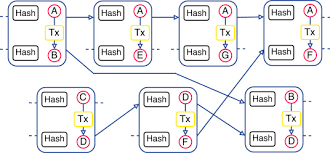
\includegraphics[scale=0.6]{Trustchain.png}
\caption{Trustchains of different network participants}
\label{fig:Trustchain}
\end{center}
\end{figure} 

\noindent{}When two agents interact with one another, they make their respective chains visible to each other and may even store information about each other's chains as well. This structure is strongly scalable, both in the number of agents in the network as well as in the number of transactions per agent. Moreover, the trustchain does not maintain a global consensus. This means that double-spends are not actually prevented, as they are in traditional blockchains. However, they are made detectable through a gossip-protocol as peers share information about other nodes' transaction histories and can subsequently be penalized through peer rejection or even by banning dishonest nodes from the network \cite{TrustChain: A Sybil-resistant scalable blockchain}. Thereby fraudulent activity is not actually prevented, but detected and punished.\vspace{1em}\\

\noindent{}\begin{center} [Trustchain and Blockchains needs a better explanation] \vspace{1em}\\\end{center}
\noindent{}In TrustChain elements of these sequences are 'linked' through hashpointers. In trustchain a transaction corresponds to a single block. Blocks in TrustChain however contain additional entries such as:

\begin{itemize}
\item Seeder public key 
\item Leecher public key
\item Upload size
\item Total amount of data contributed by seeder
\item Total amount of data consumed by seeder
\item Total amount of data contributed by leecher
\item Total amount of data consumed by leecher
\item Sequence number of transaction in the leecher's trustchain
\item Sequence number of transaction in the seeder's trustchain
\item Hash of previous block in seeder's trustchain
\item Hash of previous block in leecher's trustchain
\item Leecher's signature
\item Seeder's signature
\item Timestamp
\end{itemize}

\noindent{}\begin{center} [Explain Gossip Protocol] \end{center}

\section{Sybil Attacks and Misreports}
\label{sec:Sybil Attacks and Misreports}
\noindent{}A reputation mechanism is meant to prevent lazy freeriding by punishing defectors with a bad rating. However, there are several ways malicious actors may try to abuse the gossip protocol to misreport on previous interactions and/or exploit the incentive mechanisms of the network, in an attempt to improve their standing and increase the likelihood of receiving contributions and leech excessively. The two most prominent ways for doing this are {\it sybil attacks} and {\it misreporting attacks}. \vspace{1em}\\

\noindent{}A {\bf sybil attack} occurs when a single malicious agent creates multiple, often times large amounts of, fake identities. This agent will then attempt to exploit the control they have over the accounts in order to artificially increase the reputation score of one or more of their identities by reporting high levels of reputability through fake transactions without actually performing any work. Another approach may be to simply reduce the reputation of other honest nodes in the network to improve their own repsective standing(s). This can be done because Sybil identities can create forged reports about one another. Recall the concept of digital signatures mentioned in \ref{subsec:Blockchains and TrustChain}. Such attacks can have strongly detrimental effects on the functioning of P2P networks, especially if carried out on a large scale. If the creation of identities and forging of signatures are cheap compared to their gain, then such attacks have the potential to disrupt entire file-sharing networks [Include image of Sybil attack (Maybe the one on maxflow) ].  \vspace{1em}\\

\noindent{}A {\bf misreport attack} is performed by one or more malicious agents who do not report honestly on their own past interactions. \cite{DropEdge} have cooked up a mechanism which solves this problem quite nicely. Note that this kind of attack is curbed by digital signatures and the trustchain architecture. However, agents may still decide to drop blocks from their trustchain that do not refelct favourably upon them in a so-called {\it block-withholding attack}. Note that such an attack cannot be carried out for blocks in the middle of the chain, but only at the end of the chain, i.e. if a block in the chain is kept secret from another node then due to the hash-pointer structure, no succeeding blocks can be shown. [Maybe incluce image for this].\vspace{1em}\\ 

\noindent{}Note that the existing trustchain architecture prevents agents from misreporting about their own interaction history in the sense that nodes cannot come up with fake interactions with other nodes, due to digital signatures on each interaction that are required by both parties for a block to be considered valid. However nodes can perform what we described earlier as a block withholding attack, in which agents do not report on their full interaction history. This may lead to two agents reporting a different weight on the edge connecting the two. This problem was solved in \cite{Jetse's work}. Additionally, the decentralised nature of the network may lead to a delay in interaction dissemination, hence different agents may know about different interactions that have occurred. Consequently, each agent can form their own subjective view of the work graph. \vspace{1em}\\

\noindent{}Note that \cite{Jetse's work} have come up with a mechanism for preventing this kind of attack. It's based on a certain subset of nodes whose job it is to witness the creation of a block. These witnesses are chosen at random by taking the nodes in the network whose public keys are 'closest' to the hash of the block created. This makes it possible to prevent block-withholding attacks. \vspace{1em}\\

\noindent{}\cite{A Survey of Peer-to-Peer Network Security Issues} identify a number of other kinds of attacks on reputation systems, such as collusion attacks, eclipse attacks, DDoS attacks, poisoning the network, i.e. slow down DHT lookup by introducing useless junk into the network, Blocking traffic by not rerouting traffic, (relay nodes in Tribler), problems with TOR and tracking data packets based on the size of transaction on TrustChain (deanonymising). \vspace{1em}\\

\noindent{}\begin{center} [Talk to the guys about possible attacks on DHT, i.e. nodes query one another and redirect this query to other nodes. If there's Sybils then they could prevent this query from being rerouted and simply share the wrong file with the querying node and pocket the reputation] \vspace{1em}\\ \end{center} 

\noindent{}While there are many different kinds of attacks on P2P filesharing networks our main focus will lie on the Sybil attack problem.\vspace{1em}\\

\section{Thesis Goal}
\label{sec:Thesis Goal}
In this thesis project it is our goal to draw on mechanisms of cooperation that evolve in nature, primarily indirect reciprocity and apply it to the context of P2P file-sharing networks. We aim to devise a mathematical algorithm which exploits structural aspects of the social graph to determine which agents are cooperators and which aren't. The idea is to compose or improve upon existing reputation mechanisms in P2P file-sharing networks that reward agents for altruistic behaviour and punish freeriding. Especially important is that the algorithm be resistant to sybil and misreport attacks. By this we mean that while it is impossible to prevent sybil attacks all together we aim to bound the benefit of large scale sybil attacks such that the cost to benefit ratio of sybil attacks is bounded. Our algorithm should be able to satisfy the two conditions of what \cite{How Should We Define Goodness} identify as the {\it leading eight}: Cooperation with reputable people and defection against disreputable people should lead to an increase in reputation score, doing the opposite should reduce one's reputation. The algorithm should satisfy the requirement for transitvity of trust as well. This means, that if reports of reputability should be weighted according to the reputability of the agent doing the report. Ideally, we'd try to construct an algorithm that covers a large number of P2P social networks, ranging from social media networks such as {\it Twitter} and {\it Facebook} to common file-sharing communities. Our main focus, however will lie on the Tribler application. This leads us to the main research question, the TU Delft's Blockchain Lab focuses their study on: Is it possible to incorporate a digital counterpart to reputation in a distributed P2P filesharing network with no central authority? \vspace{1em}\\

\section{Problem Description}
\label{sec:Problem Description}
\noindent{} \begin{center} [This needs to be tidied up and merged with the Thesis Goal chapter] \vspace{1em}\\ \end{center}
\noindent{}P2P networks consist of {\it cooperative nodes} who contribute as much or more than they consume and {\it freeriders} who consume more than they contribute. A well-functioning network should then optimally cosist of more contributers than freeriders. Implementing this is a difficult problem to solve and one approach to this is Trust. In this work our goal is to devise a mechanism with which we can determine the trustworthiness/reputability of agents in a distributed p2p network called {\it Tribler}, thereby mitigating the effects of Sybil attacks on the network. We aim to extend this work to other p2p networks such as social media networks like {\it Twitter} and {\it Facebook}. In order for us to be able to attemp this we begin by introducing the respective definitions of Trust, Reputation and Accounting Mechanisms. \vspace{1em}\\

\noindent{}\cite{Bartercast: A Practical Approach to Prevent Lazy Freeriding in P2P Networks} distinguish two types of malicious agents in their network, lazy-freeriders and die-hard-freeriders, for 2 reasons. $(i)$ Practical p2p networks deployed in the real world work reasonably well, despite not having a perfect water-tight resistance to all types of attacks. $(ii)$ Only a very small proportion of users in real-life networks actually have the technical sophistication to subvert these protocols. It is therefore important to make a theoretical distinction between preventing die-hard freeriding and preventing simple lazy freeriding. \vspace{1em}\\

\noindent{}Note that it is important to mention here that we are primarily interested in distributed accounting mechanisms, i.e. those where there is no central authority that has all the information ready and are the only authority. Those types of networks have a central point of failure, administrational overhead and require their users to blindly trust an authority to control the network and ahve access to all information. \vspace{1em}\\  

\section{A mathematical Framework for Accounting Mechanisms}
\label{sec:A mathematical Framework for Accounting Mechanisms}
\noindent{}We begin by introducing a mathematical framework for the setting in which we conduct our research. We begin by defining a transaction between nodes. In \cite{Sybil-resistant Trust Mechanisms in Distributed Systems} (Otte, 2016) introduce the concept of an ordered interaction model from which an ordered interaction graph and a block graph is derived. While this is a very elegant definition for a set of transactions and the derivation of a work graph from it, it lacks the possibility of misreports and counterfeit interactions. Therefore we will not adopt it in here, but instead derive a slightly different definition of a transaction set which will be our equivalent to their ordered interaction model.\vspace{1em}\\


\begin{definition}[Network Transactions]\ \\
Let $V$ be the set of agents in the network. An interaction between two nodes $i,j\in{}V$ is given by a tuple $(i,j,w)$, whereby $w$ corresponds to the size of the transaction, i.e. the amount of data transferred from $i$ to $j$. Hence, the ordering of the two nodes in the transaction is not arbitrary, but for a transaction $t$, $pr_1(t)$ is the contributer while $pr_2(t)$ is the recipient of the work performed. Naturally, it always holds $w\geq{}0$. \vspace{1em}\\
\end{definition}

\begin{definition}[Transaction Sets]\ \\
\noindent{}As every node participates in a string of transactions that follow a given chronological order, we obtain a sequence of transactions for every node $i$, which we will refer to as transaction sets $TS_i:=(t^i_n)_{n\in\mathbb{N}_{\leq{}T_i}}$ where $t^i_n$ is the $n$-th transaction of node $i$. We write $t^i_n=(j,k,w)$ where either $j=i$ or $k=i$. $T_i$ denotes the length of $i$'s transaction set, i.e. the number of transactions $i$ has participated in thus far. It grows as time progresses.\vspace{1em}\\
\end{definition}

\begin{definition}[Transaction Function]\ \\
\noindent{}We define a transaction function $t^i$ for every node $i\in{}V$, given by 
\[
t^i:\mathbb{N}\times{}V\rightarrow{}\mathbb{R},
\]
\noindent{}where $t^i(m,j)=w$ if either $(i,j,w)=t_m^i\in{}TS_i$ or $(j,i,w)=t_m^i\in{}TS_i$. \vspace{1em}\\ 
\noindent{}It holds $t^i(m,j)\geq{}0\Rightarrow t^i_m=(i,j,w)$ and $t^i(m,j)\leq{}0\Rightarrow t^i_m=(j,i,w)$ for some $w\geq{}0$ respectively. We write $t^i(m,j)=0$ if neither $pr_1(t^i_m)\neq{}j$ nor $pr_2(t^i_m)\neq{}j$, or if $T_i<m$.\vspace{1em}\\
\end{definition}

\noindent{}In theory it should always hold:
\[
\forall{}i,j\in{}V,n\in\mathbb{N},\,t^i(n,j)=w\neq{}0:\exists{}m\in\mathbb{N},\,t^j(m,i)=-w,
\]
\noindent{}however, we will show a bit later that this need not necessarily be the case, due to a malicious strategy, called {\it misreporting}. \vspace{1em}\\
\noindent{}Now, every node has a transaction set containing all transactions it has participated in, given by a sequence
\[
TS_i=\left(t^i_n\right)_{n\in\mathbb{N}_{\leq{}T_i}}
\] 
We denote the set of all transactions as $TS:=\left\lbrace{}TS_i\,|\,i\in{}V\right\rbrace.$ \vspace{1em}\\ % $TS=\bigcup\limits_{i\in{}V}TS_i$

\noindent{}Note that a transaction can only ever go "one way". This means a single transaction cannot contain the transference of data from node $i$ to $j$ {\bf and} vice versa. \vspace{1em}\\

\noindent{}\begin{center}[Compare with Pim's work again.] \vspace{1em}\\ \end{center}

\noindent{}Given the set of all transactions $TS$, one can transform these transaction sequences into a {\it work graph}. \vspace{1em}\\

\begin{definition}[Work Graph]\ \\
A work graph is given by the tuple $G = (V, E, \omega)$, whereby $V$ is the set of vertices, i.e. agents in the network and $E$ is a set of directed edges between the community agents. An edge $(i,j)\in{}E$ pointing from node $i$ to node $j$ represents node $j$ performing work for node $i$. Although this can and sometimes is turned around.\\ The function $\omega:V\times{}V\rightarrow{}\mathbb{R}_{\geq{}0}$ denotes the weight of the edges, i.e. $w(i,j)$ represents the total amount of work performed by node $i$ for node $j$. If two nodes $i$ and $j$ are not connected then we set the edge weights $w(i,j)=w(j,i)=0$. The edges of the graph can be derived from the set of all transactions $TS$ by
\[
w(i,j) = \max\left\lbrace{}\sum\limits_{n\in\mathbb{N}}t^j(n,i), 0\right\rbrace = \max\left\lbrace{}-\sum\limits_{n\in\mathbb{N}}t^i(n,j), 0\right\rbrace
\]
and consequently, 
\[
w(j,i) = \max\left\lbrace{}\sum\limits_{n\in\mathbb{N}}t^i(n,j), 0\right\rbrace = \max\left\lbrace{}-\sum\limits_{n\in\mathbb{N}}t^j(n,i), 0\right\rbrace
\]
\end{definition}

\noindent{}In the definition above the work graph is directed and unidirectional, where the weight of the edges is given by the net data flow in between two nodes. The edge is directed toward the node that has a positive deficit in the bilateral relationship. Note that there can only be a single edge connecting two nodes, which points from one to the other. Note that there is one drawback to this approach, which lies in the fact that if two agents have donated the same amount of resources to one another then the weight of the edge connecting them is zero. Hence, the edge has "disappeared" and the nodes appear to be disconnected again. This will prove problematic at times and will enable a certain type of attack which we call a serial sybil attack in \ref{subsec:Accounting Mechanisms}. \vspace{1em}\\

\begin{center} [Include example with table of transactions and the following work graph] \vspace{1em}\\ \end{center}

\noindent{}Note that there are several ways of aggregating transactions into a work graph and we have chosen the former as it is the simplest way that does not bring about any problems later on. One can make the graph bidirectional with double edges in between two nodes, in which case the edge weights are derived as 

\[
w(i,j) = \sum\limits_{n\in\mathbb{N}}\max\left\lbrace{}t^j(n,i), 0 \right\rbrace = \sum\limits_{n\in\mathbb{N}}\max\left\lbrace{}-t^i(n,j),0\right\rbrace 
\]
\noindent{}and
\[
w(j,i) = \sum\limits_{n\in\mathbb{N}}\max\left\lbrace{}t^i(n,j), 0 \right\rbrace = \sum\limits_{n\in\mathbb{N}}\max\left\lbrace{}-t^j(n,i),0\right\rbrace
\]
\noindent{}It may be somewhat counterintuitive for edges to be pointing from the recipient to the contributor. This is done with a particular set of reputation mechanisms in mind that we will elaborate on further later on. It may also be reasonable to invert the edges in between nodes in the graph, depending on the application. In that case we obtain

\[
w(i,j) = \sum\limits_{n\in\mathbb{N}}\max\left\lbrace{}t^i(n,j), 0 \right\rbrace = \sum\limits_{n\in\mathbb{N}}\max\left\lbrace{}-t^j(n,i),0\right\rbrace.
\]

\noindent{}Note that in our case work performed (weight of edges) corresponds to the amount of data transferred from one node to another, by seeding (leaching respectively) in the Tribler network. But this notion can be extended to any arbitrary kind of p2p network such as the {\it Twitter} or {\it Facebook} networks, in which the connections between agents correspond to follow or friendship relations. The weights of these edges could then, for instance, be determined by the number of likes and/or retweets a user receives from a follower/friend. \vspace{1em}\\

\noindent{}In order for an agent to discover the work graph, it has to query nodes in the network for their transaction history. Agents will share their own transaction set with a querying node and demand their respective set in turn. 

\noindent{}We will not elaborate much further the details of information dissemination and simply assume that there exists some protocol by which these transaction sets are distributed in the network. The fact that no agent in the network has full knowledge of all other nodes' transaction sets implies that the objective work graph above is not available to any agent in the network. Agents have some subset of knowledge of past interactions in the network based on which they can form their own personal view of the network. Next, we introduce the notion of agent information.

\begin{definition}[Agent Information]\ \\
Every agent $i$ keeps a private history of its own transactions with other peers $TS_i$ from which it can derive a set of tuples corresponding to all edges it is connected to
\[
H_p(i):=\left\lbrace{}w_i(i,j)\,|\, j\in{}V\right\rbrace \cup \left\lbrace{}w_i(j,i)\,|\, j\in{}V\right\rbrace .
\]
\noindent{}The $H_p$ does not require any queries about the transaction sets of other nodes, as all incoming and outgoing edges of $i$ can be directly derived from $TS_i$ as denoted above in the definition about the obective work graph. \vspace{1em}\\

\noindent{}The information about the transactions between other nodes is only available through reports. Nodes report a transaction set to $i$ from which $i$ can derive a set of edge weights, belonging to the edges connecting other nodes in the network. However, the sets $i$ receives may not always be perfectly identical. Time delays, for insance could lead to $i$ receiveing one transaction set before a particular transaction occurs and another thereafter. Hence $i$ the edge weights $i$ derives from reports my differ depending on the reports. This means that any edge between two nodes will be assigned a tuple of values as denoted below.  
\[
H_r(i):=\left\lbrace{}(w_i^j(j,k),w_i^k(j,k))\,|\,j,k\in{}V\right\rbrace
\]
whereby $w_i^j(j,k)$ denotes the amount of work $j$ reports to have received from $k$ and $w_i^k(j,k)$ is the amount of work $k$ reports to have received from $k$. 
\end{definition}

\noindent{}From these reports about the edges and nodes in the graph an agent can subsequently construct their own subjective view of the work graph.

\begin{definition}[Subjective Work Graph]\ \\
A subjective work graph from the perspective of node $i$ is given by $G_i=(V_i,E_i,w_i)$ where $V_i\subset{}V$ and $E_i\subset{}E$. For $(j,k)\in{}E_i$ for which $i\not\in\left\lbrace{}j,k\right\rbrace$ we assign the edge $(j,k)$ both of the weights $w_i(j,k) = (w_i^j(j,k), w_i^k(j,k))$ as reported by $j$ and $k$ respectively. For $i=j$ or $i=k$ we use the edges $w_i^i(i,j)=w(i,j)$ and $w_i^i(j,i)=w(i,j)$. These are the edges $i$ does not have to rely on reports for.  
\end{definition}

\noindent{}\begin{center} [Include image of subjective work graph with doule edge weights...] \vspace{1em}\\ \end{center}

\noindent{}Recall that it was our goal to incentivise cooperative behaviour by a method of indirect reciprocity that is resistant to sybil and misreport attacks. So far, we have not yet defined what it means to be cooperative and what it means to be a lazy freerider.\vspace{1em}\\

\begin{definition}[Lazy freeriding]\ \\
Given an agent $i$ with respective transaction set $TS_i$, we say that $i$ is a lazy freerider if the ratio of total up-to download exceeds some arbitrary lower bound $c\in{}[0,1]$. 

\[
\frac{\sum\limits_{j\in{}V}\sum\limits_{n\in\mathbb{N}}\max\left\lbrace{}t^i(n,j), 0\right\rbrace}{\sum\limits_{j\in{}V}\sum\limits_{n\in\mathbb{N}}-\min\left\lbrace{}t^i(n,j), 0\right\rbrace}\leq{}c
\]

\noindent{}Alternatively, we can say that someone is a lazy freerider if their net contribution made to the rest of the network exceeds a lower bound $c' < 0$.

\[
\sum\limits_{j\in{}V}\sum\limits_{n\in\mathbb{N}}t^i(n,j)\leq{}c' 
\]
\end{definition}

\noindent{}A node can discover and expand their own subjective work graph by running random walks along the edges of their existing subjective work graph. When a random walk reaches a node it requests that nodes trustchain. \vspace{1em}\\

\noindent{} \begin{center} [Make sure to explain this properly, also expand on what a random walk really is] \vspace{1em}\\ \end{center}
\noindent{}Nodes have complete autonomy over their own transaction sets. This means that agents can add transactions to their sets which have not actually occured. Nodes can drop certain unfavourable transactions from their sets when making a report, or simply refuse to report their transaction set entirely. All of these ways of being dishonest fall under the definition of a {\it misreport}, which leads to the definition below.

\begin{definition}[Misreport]\ \\
Given a subjective work graph $G_i=(V_i,E_i,w_i)$ and two nodes $j,k\in{}V_i$ with respective transaction sets $TS_j,TS_k$. A misreport between $j$ and $k$ has occurred if 

\[
\neg \left(\forall{} n\leq{}T_j\,\exists m\leq{}T_k:\,t^j(n,k)=-t^k(m,j)\,\,\wedge\,\,\forall{} n\leq{}T_k\,\exists m\leq{}T_j:\,t^k(n,j)=-t^j(m,k)\right).
\]

\noindent{}In other words this means that a misreport has occurred if the transaction set of $k$ contains an interaction with $j$ that is not in the transaction set of $j$, or vice versa. This may have happened because nodes $j$ and $k$ were queried at different times or because either of the nodes $j$ or $k$ either added a transaction (that did not actually occur), or removed a transaction (that actually happened) from their transaction set. This means that from the perspective of $i$ a misreport between $j$ and $k$ has occurred if $(w_i^j(j,k),w_i^k(j,k))\in{}H_r(i)$ and

\[
w_i^j(j,k)\neq{}w_i^k(j,k)
\] 

\noindent{}This means that in the subjective work graph $G_i$ the edge $(j,k)$ will be labelled with two different edge weights.
\begin{center}[Include image of graph with misreport] \vspace{1em}\\ \end{center}

\noindent{}The problem with a misreport is that it is not clear which agent committed the misreport. Generally, agents perform misreports with the intention of boosting their own reputation, by either adding transactions that make them seem more cooperative or removing transactions in which they were the recipient of some work. We will return to this concept later on in the form of mechanisms to prevent or punish this type of behaviour. \vspace{1em}\\
\end{definition}
\noindent{}Note that these reports do not have to be true. Misreporting is in fact a popular attack on P2P networks with no central authority. This is a concept we will delve into more deeply later. \vspace{1em}\\

\begin{definition}[Misreport]\ \\
Nodes can lie about their transactions with their peers and spread false information about their own transaction history. This means an agent $j$ has the ability to manipulate the subjective work graph of another node $i$. Given the subjective  $(V_i,E_i,w_i)$.  For an agent $j$ take the sets of edges $E_{-j}=\left\lbrace{}(x,y)|(x,y)\in{}E,x\neq{}j,y\neq{}j\right\rbrace$ and $E_{j}=\left\lbrace{}(x,y)|(x,y)\in{}E,x=j\,\vee\,y=j\right\rbrace$. A misreport attack by agent $j$ on agent $i$ would be given by a $\sigma=(V_i,E_i,w_i')$, where $w_i'(k,l) = w_i(k,l)$ if $l,k\neq{}j$ and $w_i'(k,l) = (w^k_i(k,l), w^l_i(k,l))$ where $w^k_i(k,l)\neq{}w(k,l).$ 
\end{definition}

\noindent{}Recall that the subjective work graph is based on agents reporting their transaction sets $TS$ defined above. We find that a misreport attack by agent $j$ is confined to $TS'_j\subset{}TS_j$. \vspace{1em}\\

\noindent{}A node holding a particular resource will receive requests to share the given resource by a set agents in the network, which we referred to earlier as a swarm of leechers. In this model \cite{} refer to this as a choice set.

\begin{definition}[Choice Set]
Let $C_i\subset{}V_i\backslash{}\left\lbrace{}i\right\rbrace$ denote the choice set for agent $i$. The choice set can be of variable size depending on how many nodes are requesting work from $i$. 
\end{definition}

\noindent{}Every node will now use their subjective work graph in order to determine a score of reputability/cooperativeness for every node, using some algorithm. This is known as an acounting mechanism.

\begin{definition}[Accounting Mechanism]
An accounting mechanism $S^M$ of agent $i$, based on an algorithm $M$, takes as input a subjective work graph $G_i$ (from the perspective of $i$) and a choice set $C_i$ and determines a score $S^M_j(G_i,C_i)$ for every agent $j\in{}C_i$ or $V_i$. 
\end{definition}

\noindent{}The agent now has to decide whom to contribute to based on their respective subjective work graph, choice set and accounting mechanism. This is what we call allocation policies. \vspace{1em}\\

\begin{definition}[Allocation Policy]\ \\
Given a subjective work graph $G_i$, a choice set $C_i$ and a set of accounting scores $S^M(G_i,C_i):=\left\lbrace{}S^M_j(G_i,C_i)\,|\,j\in{}C_i\right\rbrace$ an allocation policy is a mapping $A_i(S^M(G_i,C_i))\subset{}C_i$, where $A_i$ determines which agent(s) in the choice are to receive some work from $i$.
\end{definition}

\noindent{}There are infinite possible different allocation policies. We will introduce a few here.

\begin{definition}[Ranking Policy]\ \\
Given a reputation algorithm $M$, subjective work graph $G_i$ and choice set $C_i$ of agent $i$ the ranking policy is given by $A_i(S^M(G_i,C_i))=\argmax{\left\lbrace{}S^M_j(G_i,C_i)\,|\,j\in{}C_i\right\rbrace}$. This means $i$ decides to perform all of its possible work for the node with the highest accounting value in the choice set. If there are several nodes who all have the same (highest) accounting mechanism values, then the "winner" is chosen ata random amongst them.
\end{definition}

\noindent{}A contributing node may also decide to divide its resources into equally sized chunks and to share these among several nodes in its choice set. 

\begin{definition}[Banning Policy]\ \\
Given a reputation algorithm $M$, subjective work graph $G_i$ and choice set $C_i$ of agent $i$ the ranking policy is given by $A_i(S^M(G_i,C_i))=\left\lbrace{}j\in{}C_i\,|\,S^M_j(G_i,C_i)\geq\delta\right\rbrace$ for some arbitrary, but fixed $\delta>0$. This means $i$ decides to contribute to every node in its choice set whose accounting value exceeds a given lower bound. 
\end{definition}

\begin{definition}[Top $n$ policy]\ \\
Given a reputation algorithm $M$, subjective work graph $G_i$ and choice set $C_i$ of agent $i$ the ranking policy is given by $A_i(S^M(G_i,C_i))=\argmax\limits_{C'_i\subset{}C_i \,\, |C_i|=n}{\left\lbrace{}S^M_j(G_i,C_i)\,|\,j\in{}C_i\right\rbrace}$
\end{definition}

\noindent{}The upper definitions can be refined in such a way that the possible contribution made by $i$ is divided into differently sized portions which are then distributed among different agents in the choice set, whereby the contribution each agent receives is weighted by its reputation/allocation value in relation to the values of the remaining nodes. The two below are example of such allocation policies.\vspace{1em}\\

\begin{definition}[Distribution Policy]\ \\
Given a reputation algorithm $M$, subjective work graph $G_i$ and choice set $C_i$ of agent $i$ the distribution policy is given by $A_i(S^M(G_i,C_i))=C_i$, where every node $j\in{}C_i$ receives 
\[
\tilde{\omega}\cdot\frac{S^M_j(G_i,C_i)}{\sum\limits_{k\in{}C_i}S^M_k(G_i,C_i)}
\]
\end{definition}

\begin{definition}[Rank-weighted Distribution Policy]\ \\
Given a reputation algorithm $M$, subjective work graph $G_i$ and choice set $C_i$ of agent $i$, we call $r_{S^M(G_i,C_i)}:C_i\rightarrow\left\lbrace{}1,\ldots,|C_i|\right\rbrace$ the ranking, where $r_{S^M(G_i,C_i)}(k)$ denotes the rank of node $k$ in $C_i$, i.e. if $k$ has the second largest accounting value in $C_i$ then $r_{S^M(G_i,C_i)}(k)=2$. If several nodes in $C_i$ have the same accounting values they are assigned the same values of $r_{S^M}$. However, unlike in the case of spearman's rank correlation the following node then has rank 3. The unweighted distribution policy is given by $A_i(S^M(G_i,C_i))=C_i$, where every node $j\in{}C_i$ receives
\[
\tilde{\omega}\cdot\frac{r_{S^M(G_i,C_i)}(j)}{\sum\limits_{k\in{}C_i}r_{S^M(G_i,C_i)}(k)}
\]
\end{definition}

\noindent{}Up until now this problem seems like a relatively easy one to solve. There are a number of different graph theoretical centrality measures that would be suitable for such an algorithm, that come to mind. However, an additional complication arises in the context on online P2P networks. Agents can create multiple identities that appear as independent actors to all other agents in the network. These agents can create transactions in their transaction sets that have not actually occurred. Because both transaction sets in this case contain the same transactions this does not qualify as a misreport attack, instead we label this kind of behaviour as a "sybil attack".

\begin{definition}[Sybil Attack]\ \\
Given an objective work graph $G=(V,E,w)$, a sybil attack by agent $j\in{}V$ is given by a set of $n$ new identities $S=\left\lbrace{}s_{j_1},\ldots{},s_{j_n}\right\rbrace$, a set of edges $E_S\subset{}S\cup\left\lbrace{}j\right\rbrace\times{}S\cup\left\lbrace{}j\right\rbrace$ with edge weights $w_S:S\cup{}\{j\} \times S\cup{}\{j\}\rightarrow{}\mathbb{R}$. Additionally, there must be a set of attack edges $E_{attack}$, i.e. $w_{attack}:V\times{}S\cup\left\lbrace{}j\right\rbrace\rightarrow\mathbb{R}_{\geq{}0}$. We label a sybil attack by node $j\in{}V$ with $n$ fake identites $\sigma^n_j$. \vspace{1em}\\

\noindent{}The new work graph after the sybil attack is given by $G':=G\downarrow\sigma^n_j=(V',E',w')=(V\cup{}S,E\cup{}E_S\cup{}E_{attack},w')$. Attack edges correspond to real transactions in which the attacker makes a legitimate donation to some nodes in the honest part of the network from one or more of the nodes they create. We define a sybil attack on a subjective work graph equivalently. Note that it is common for the sybil region to be densely connected, forming a separated cluster in the network. The obvious way to mitigate these is by community detection algorithms that detect densely connected regions in the work graph. However, sybil attacks can take many different forms and shapes and therefore this is not a feasible solution for {\it all} types of sybil attacks. \vspace{1em}\\
\end{definition}

\noindent{}Note that in \cite{On the Sybil-Proofness of Accounting Mechanisms} the authors differentiate between an {\it active} and a {\it passive} sybil attack. In a passive sybil attack, attack edges are only connected to one and the same node, i.e. $w'(s,k)=0$ f.a. $s\in{}S,k\in{}V\backslash\lbrace{}j\rbrace$. In an active sybil attack every node in the sybil region may be connected to the honest region of the network. In \cite{Sybil-resistant Trust Mechanisms in Distributed Systems} a sybil attack is defined such that it is perpetrated by a set of nodes $J\subset{}V$. This was done to combine both definitions of active and passive sybil attacks in one. We find this definition slightly awkward as it seems to combine sybil attacks with collusion attacks in one definition. Hence, our definition above deviates from the existing ones a bit.\vspace{1em}\\ 
\begin{center}[Include image of active and passive sybil attacks!] \vspace{1em}\\ \end{center}

\begin{figure}[H]
\begin{center}
\includegraphics[scale=0.5]{"Sybil Region".jpg}
\caption{Sybil Region}
\label{fig:Sybil Region}
\end{center}
\end{figure}

\noindent{}Seeing as in the sybil attack defined above, the work graph does not reveal who the sybil attacker is and who their fake identities are (this only the case in \cite{Sybil-resistant Trust Mechanisms in Distributed Systems} and in \cite{On the Sybil-Proofness of Accounting Mechanisms}), we can also drop the $j$ from $\sigma^n_j$. \vspace{1em}\\

\subsection{Sybil Attack Profit}
\label{subsec:Sybil Attack Profit}
\noindent A Sybil attack is called beneficial if the attacking agent or one of its sybils is chosen to receive some work when without the attack it wouldn't have been. There's 4 ways of how this can be the case. 

\begin{definition}[Beneficial Attacks]
An attack by agent $j$ is beneficial if for some agent $i$ with choice set $C_i$, subjective work graph $G_i$, accounting mechanism $S^M$ and allocation policy $A_i$ that would pick some agents $A_i(S^M(G_i,C_i))\subset{}V$, we obtain one of 4 outcomes 
\begin{itemize}
\item[$\cdot$] j's score is increased such that $j\in{}A_i(S^M(G'_i,C'_i))$ when before $j\not\in{}A_i(S^M(G'_i,C'_i))$
\item[$\cdot$] Other agents' scores are lowered such that $j\in{}A_i(S^M(G'_i,C'_i))$ when before $j\not\in{}A_i(S^M(G'_i,C'_i))$
\item[$\cdot$] A sybil $s$ is assigned a score such that $s\in{}A_i(S^M(G'_i,C'_i))$ when before $s\not\in{}A_i(S^M(G'_i,C'_i))$
\item[$\cdot$] Other agents' scores are lowered such that $s\in{}A_i(S^M(G'_i,C'_i))$ for some sybil $s$ when before $s\not\in{}A_i(S^M(G'_i,C'_i))$
\end{itemize}
\end{definition}
\noindent{}However the upper conditions may be satisfied for a single attacking node, or for several. They may also hold true for multiple nodes $i$ from which the attacking agents could leech. Additionally, one or more of them may also still be satisfied after one or more of the attackers have received some work. \vspace{1em}\\

\noindent{}Hence, we see that some sybil attacks may be more beneficial than others depending on how much more work the attacker can consume than they were actually entitled to before the attack occurred. We now want to introduce an exact definition of {\it how} beneficial a sybil attack is, which will be determined by the relation of work put into the attack versus the amount of work that the attacker(s) can gain from it.\vspace{1em}\\

\begin{definition}[Sybil Attack Profit]\ \\
Given an objective and a subjective work graph $G:=(V,E,w)$, $G_i:=(V_i,E_i,w_i)$, let $\sigma_j^n$ be a sybil attack of size $n\in\mathbb{N}$ with Sybil region $S=\left\lbrace{}s_{j1},\ldots,s_{jn}\right\rbrace$, whereby $n$ is not fixed. Take $G':=(V',E',w')$ and $G_i':=(V_i',E_i',w_i')$ as defined above. We label $\omega_{-}^{n}$ as the amount of work invested into the sybil attack, i.e. the collective weight of all outgoing edges from the sybil region. 

\[
\omega_{-}^{n} = \sum\limits_{v\in{S}\cup\{j\}}\sum\limits_{u\in{}V}^{}w(v,u)
\]

\noindent{}Note that at the moment of the sybil attack the newly created nodes, i.e. the sybil nodes have not received any work from other nodes in the network yet. This, of course, does not hold for $j$ itself as it may have already participated in the network before launching the sybil attack. In the case of a passive sybil attack it even holds $w(u,v)=0$ f.a. $u\in{}V\backslash{}\left\lbrace{}j\right\rbrace$, $v\in{}S$.\vspace{1em}\\

\noindent{}Of course, in the case of a passive sybil attack this definition is slightly simpler as all attack edges are connected to $j$ and no other sybil node. The cost of a sybil attack is then given by 

\[
\omega_{-}^{n} = \sum\limits_{u\in{}V}^{}w(j,u)
\]

\noindent{}This is the amount of actual work the attacker has to invest into the attack, in order to boost its own and its sybils reputation, relative to the rest of the network, and consequently obtain work from the rest of the network. The edges in the work graph corresponding to this work performed are what we called {\it attack edges}. Note that these edges are indispensable for a sybil attack. If no such edges exist then no node in the sybil region, including $j$ can increase their accounting values from the perspective of any node outside of the sybil region. For this to hold true, we set a requirement for our accounting mechanisms later, known as path-responsiveness.  \vspace{1em}\\

\noindent{}Inversely, we should define the reward/profit $\omega_{+}^{n}$ of a sybil attack by the aggregated amount of work, all nodes in the sybil region can collectively consume after the attack has been carried out. If the attack enables the sybils to consume much more data than they collectively performed, the attack will be considered detrimental to the network and beneficial for the attacker. Based on our definition of lazy freeriding in section \ref{sec:Problem Description}, we will want to determine $\frac{\omega_{+}^{n}}{\omega_{-}^{n}}$. \vspace{1em}\\

\noindent{}However, computing the value of $\omega_{+}^{n}$ turns out to be a rather difficult task. There are a number of different factors this value depends on, such as the accounting mechanism and the allocation policy of agents in the network as well as the state of the interaction graph. More importantly, it depends on the dynamic of the interaction graph as time progresses and interactions between different agents occur. Other agents participating in transactions, even if these don't involve the attackers themselves, will affect the reputation values of the attackers and therefore also the value of $\omega_{+}^{n}$. \vspace{1em}\\

\noindent{}In particular, this value turns out to be probabilistic in nature. A node $j$ that queries another node $i$ for some data will be served if at the given point in time it happens to be the node with the highest accounting value in $i$'s choice set, provided $i$'s allocation policy is "winner-takes-all". More generically, if it's in the set of nodes determined by the allocation policy. This, of course, does not only depend on $j$'s accounting value, but on who else happens to query $i$ at this given point, which $j$ has no control over. In order for us to be able to gauge this, we introduce an interaction model among agents, with the intent to approximate the dynamics of real-world p2p networks. In fact, we assume a model in which the choice set will be random, following a given distribution, explained below.  \vspace{1em}\\ 

\subsection{Interaction Model}
\label{subsec:Interaction Model}
\noindent{}We say that the network operates in rounds (for simplicity). In each round, every honest node $k$ will (with a given probability $q$, $Ber(q)$) query some other randomly chosen node $i$ in the network. The node that is queried is chosen following the uniform distribution with probability $\frac{1}{|V\backslash\left\lbrace{}k\right\rbrace{}|}$. Every honest node that has been queried will respond by doing some work for the node with the highest accounting value in its choice set. For simplicity, the amount of work will be a fixed value $\tilde{w}$. Let $C_i$ be the set of all agents, requesting some work from agent $i$ in a given round. Then it follows $|C_i|\sim\mathcal{B}in(V\backslash\left\lbrace{}i\right\rbrace{},\frac{q}{|V|-1})$. Due to independence of the two random variables (uniform and bernoulli) we can multiply the probabilities and obtain the binomial distribution. \vspace{1em}\\

\noindent{}There are some inevitable inaccuracies in this model. In real file-sharing networks nodes query other nodes, based on the files they are interested in. To assume that nodes are chosen with equal probability is not $100\%$ realistic, as there may be nodes holding more sought-after files than others. Some agents may not hold any files at all and will therefore not receive any queries at all. We also disregard the possibility of nodes going offline and therefore not responding to queries and/or not querying other nodes in the network. A fixed size $\tilde{w}$ of every transaction is also somewhat unrealistic as files vary in size, but we see it as a necessary restriction for the model. Lastly, the notion that the network operates in rounds is also somehwat contrived as real-world networks are continuous and requests for files do not come in rounds. \vspace{1em}\\

\noindent{}We assume that all agents follow the winner-takes-all allocation policy as it is the most resistant to large-scale sybil attacks of all methods for distributing data among agents in the choice set, which do not "split" the $\tilde{\omega}$. This is, because it obviously holds for all $n\geq{}1$ and any randomly put-together choice set $C_i$ of size greater than $n$, as well as a sybil region $S$

\[
\mathbb{P}\left(\argmax\limits_{k\in{}C_i}\left(S_k^M(G_i,C_i)\right)\in{}S\right) \leq \mathbb{P}\left(\argmax\limits_{C_i'\subset{}C_i,\,|C_i|=n}\left\lbrace{}S_k^M(G_i,C_i)\,|\,k\in{}C_i\right\rbrace\cap{}S \neq \varnothing\right).
\]

\noindent{}This is obvious, as the probability of a sybil node being the highest-ranking in $C_i$ is lower than the probability of one or more sybil nodes belonging to the highest-ranking $n$ nodes, when the choice set is generated as given by the model above. Hence the probability of the attacker obtaining at least $\tilde{\omega}$ units of work is lowest in the case of the winner-takes-all allocation policy, independently of the accounting mechanism at hand, provided it satisfies path-responsiveness and positive-report-responsiveness.\vspace{1em}\\

\noindent{}The reason we claim that path-responsiveness and positive-report-responsiveness need to be satisfied for this to hold is that they imply the necessity of attack edges for sybil attacks to be beneficial. This is turn implies that "actual work" needs to be performed by an attacker, which makes it impossible to obtain arbitrarily high accounting values for the sybils. This justifies the upper inequality. \vspace{1em}\\

\noindent{}Since, the upper inequality holds for any arbitrary $i$, it then holds for the entire network, i.e.

\[
\mathbb{P}\left(\bigcup\limits_{i\in{}V\backslash\lbrace{}j\rbrace}\argmax\limits_{k\in{}C_i}\left(S_k^M(G_i,C_i)\right)\in{}S\right) \leq \mathbb{P}\left(\bigcup\limits_{i\in{}V\backslash\lbrace{}j\rbrace}\argmax\limits_{C_i'\subset{}C_i,\,|C_i|=n}\left\lbrace{}S_k^M(G_i,C_i)\,|\,k\in{}C_i\right\rbrace\cap{}S\neq\varnothing\right). \vspace{1em}\\
\] 

\noindent{}Note that the same inequalities hold for the banning policy and every other policy which chooses a subset of nodes from the choice set, based on their accounting values, provided, of course, it favours nodes with higher values to nodes with lower values. So long as the amount of data $\tilde{\omega}$ is not split among several agents in the choice set, this is also an upper bound for the amount of work an attacker can expect to consume.\vspace{1em}\\

\noindent{}An attacker with sybil region $S$ will be able to obtain at most $(S|+1)\cdot{}\tilde{\omega}$ units of work in a single round. However, if $\tilde{\omega}$ is split among, for instance, the $n$ highest ranking agents in $i$'s choice set, an attacker will not be able to receive more than at most $\frac{|S|+1}{n}\cdot\tilde{\omega}$ units of work in any given round. In this case, it would be most strategic for an attacker to target other nodes with at most $n$ sybils at a time. \vspace{1em}\\ 

\noindent{}The problem here is that while the upper bound for the amount a sybil attacker can consume in one round is higher for the winner-takes-all policy than for the distribution policy, the probability of a sybil node being served by a node $i$ is higher for the distribution policy. Hence it is not clear whether the average consumption of the sybil attackers per round will be higher or lower. For the winner-takes-all policy we have an average data consumption of

\[
\sum\limits_{s\in{}S\cup\left\lbrace{}j\right\rbrace}\tilde{\omega}\cdot\mathbb{P}\left(s\in{}\argmax\limits_{k\in{}C_i}\left(S_k^M(G_i,C_i))\right)\right)
\] 

\noindent{}and for the top-n distribution policy we obtain the average payoff

\[
\sum\limits_{s\in{}S\cup\left\lbrace{}j\right\rbrace}\frac{\tilde{\omega}}{n}\cdot\mathbb{P}\left(s\in\argmax\limits_{C_i'\subset{}C_i,\,|C_i|=n}\left\lbrace{}S_k^M(G_i,C_i)\,|\,k\in{}C_i\right\rbrace\right).
\]

\noindent{}We assume that the sybil nodes do not have full knowledge on the state of the interaction graph and that targeted attacks are therefore impossible. We therefore assume that sybil attackers have no better option than to leech from randomly chosen nodes in the network. Hence we find that the probabilities summed above are all the same and we therefore obtain the following values for the expected amount of data an attacker can leech.
\[
(|S|+1)\cdot\tilde{\omega}\cdot\mathbb{P}\left(s\in{}\argmax\limits_{k\in{}C_i}\left(S_k^M(G_i,C_i))\right)\right)
\]
\noindent{}and
\[
(|S|+1)\cdot\frac{\tilde{\omega}}{n}\cdot\mathbb{P}\left(s\in\argmax\limits_{C_i'\subset{}C_i,\,|C_i|=n}\left\lbrace{}S_k^M(G_i,C_i)\,|\,k\in{}C_i\right\rbrace\right)
\]

\noindent{}At this point we find that it is not clear which allocation policy returns higher values for sybil attackers, due to the reasons explained above. The upper values now depend the accounting mechanism employed and are therefore inconclusive. However, we showed that in the extreme case the distribution allocation policy provides a stricter upper bound for this value and is therefore better at mitigating sybil attacks than the winner-takes-all allocation policy. At least in bounding the extremes of sybil attack returns. Hence, it is not clear which allocation policy is most effective at mitigating sybil attacks for generic accounting mechanisms.\vspace{1em}\\

\noindent{}There are other reasons an allocation policy that "splits" the value of $\tilde{\omega}$ among nodes in the choice set may be advantageous, such as the fact that it will lead to a more equal distribution of data among the network's participants. The goal is, of course for an allocation policy to yield a fair distribution of data among all agents in the network, while simultaneously preventing lazy freeriding and mitigating the effect of sybil attacks. In order for us to determine which allocation policy is most effective in achieving a fair distribution of data while preventing lazy freeriding, we simulate different filesharing networks with different accounting mechanisms and allocation policies.\vspace{1em}\\

\subsection{Experimental Evaluation}
\label{subsec:Experimental Evaluation}
\noindent{}We simulate a network with 100 honest nodes, query probability $0.7$ and $\tilde{\omega}=1$. We evaluate a number of different accounting mechanisms, such as the personalised PageRank algorithm \cite{A Random Walk Based Trust Ranking in Distributed Systems}, a degree-based accounting mechanism given by 
\[
S^{deg}_k(G_i,C_i)=\sum\limits_{u\in{}V\backslash\{k\}}\omega(k,u) - \sum\limits_{u\in{}V\backslash\{k\}}\omega(u,k),
\]
\noindent{}and an accounting mechanism that assigns all nodes $0$s. For allocation policies, we investigate the winner-takes-all policy, top-$n$ (with and without distribution), whereby we choose $n=4$, as well as the rank-weighted distribution policy. We run our simulation for 100 rounds and determine the up- to download ratios of nodes in the network. It might seem counter-intuitive to assume only honest nodes in such a simulation, as we are investigating which allocation policy will lead to a fairer distribution of data while also effectively preventing lazy-freeriding. \vspace{1em}\\

\noindent{}However, we find that we do not need to actively simulate freeriders. Due to the bernoulli distribution determining which nodes will query other nodes in the network for data and the uniformity of their choice over the whole network probabilistic nature of our model some agents will automatically not be queried for data as much as others. The number of queries a node will obtain as well as the number of queries a node will make will then follow an approximate Binomial distribution which means that the ratio of queries made to queries received will with a fairly large standard deviation, therefore leading to nodes that have received far fewer queries than they have made, and vice versa. We consider this an effective simulation of freeriders and obtain the following distributions for the amount of queries made and received. \vspace{1em}\\

\begin{figure}[H]
\begin{center}
\includegraphics[scale=0.6]{"Queries Count".png}
\end{center}
\end{figure}

\noindent{}In the graphs above we also find that the absolute values of queries nodes have received minus the queries they have made varies from values as small as -100 to values as large as 75. This indicates that the spectrum of altruism in the network is very wide with approximately as many nodes with a positive net value in number of queries as nodes with a negative net. Hence, depending on which we have a fair number of (attempted) lazy freeriders as well as cooperators. \vspace{1em}\\

\noindent{}Next we investigate which different allocation policies are best in achieving a fair distribution of data in the network, while preventing lazy freeriding. For this we run the same network simulation for the accounting mechanisms and allocation policies mentioned above. We obtain the following set of data distributions.

\begin{figure}[H]
\begin{center}
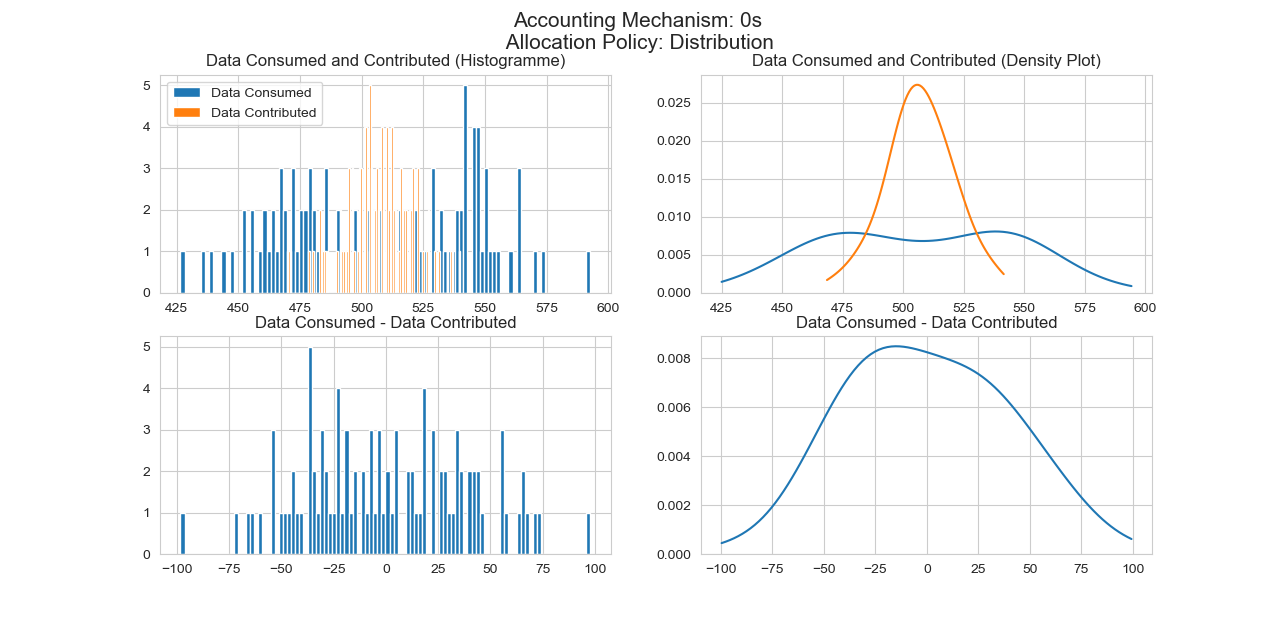
\includegraphics[scale=0.4]{Acc_0s_Dist.png}
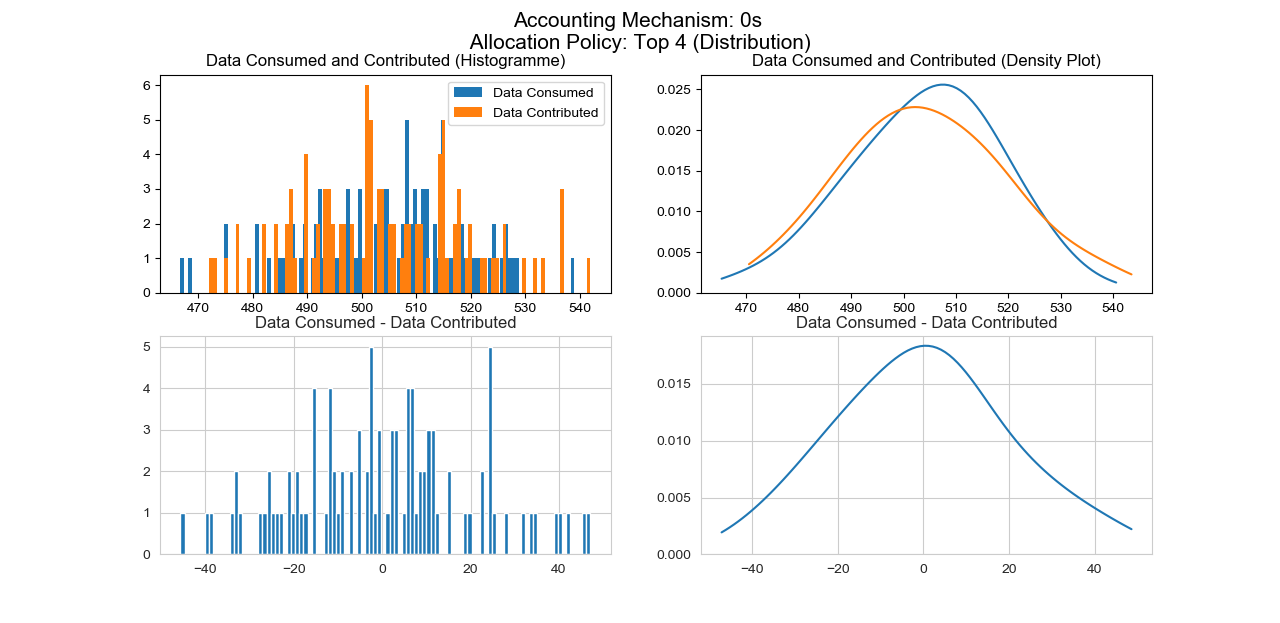
\includegraphics[scale=0.4]{Acc_0s_Top_4_Dist.png}
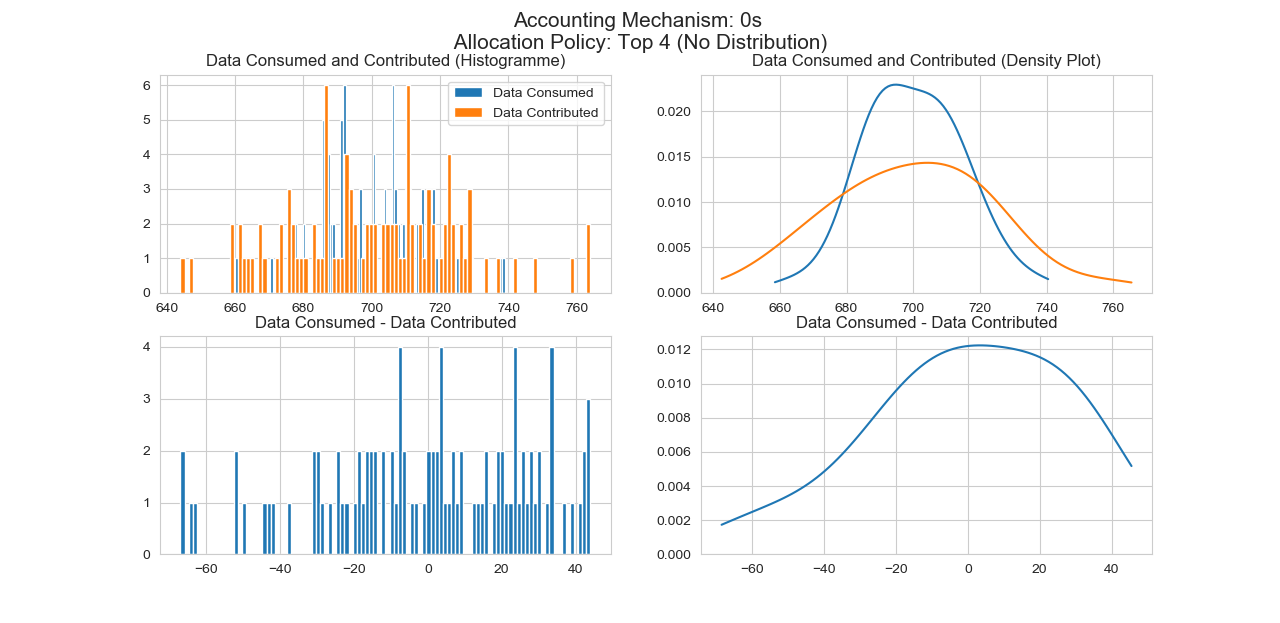
\includegraphics[scale=0.4]{Acc_0s_Top_4_No_Dist.png}
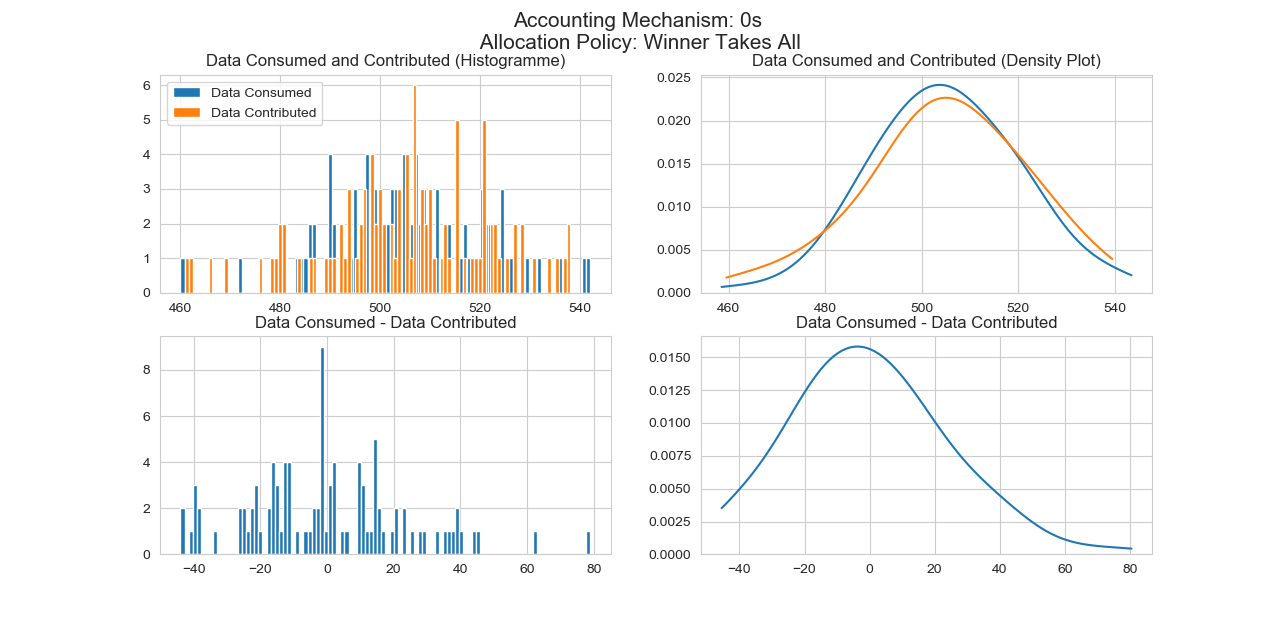
\includegraphics[scale=0.4]{Acc_0s_Winner.png}
\end{center}
\end{figure}

\begin{figure}[H]
\begin{center}
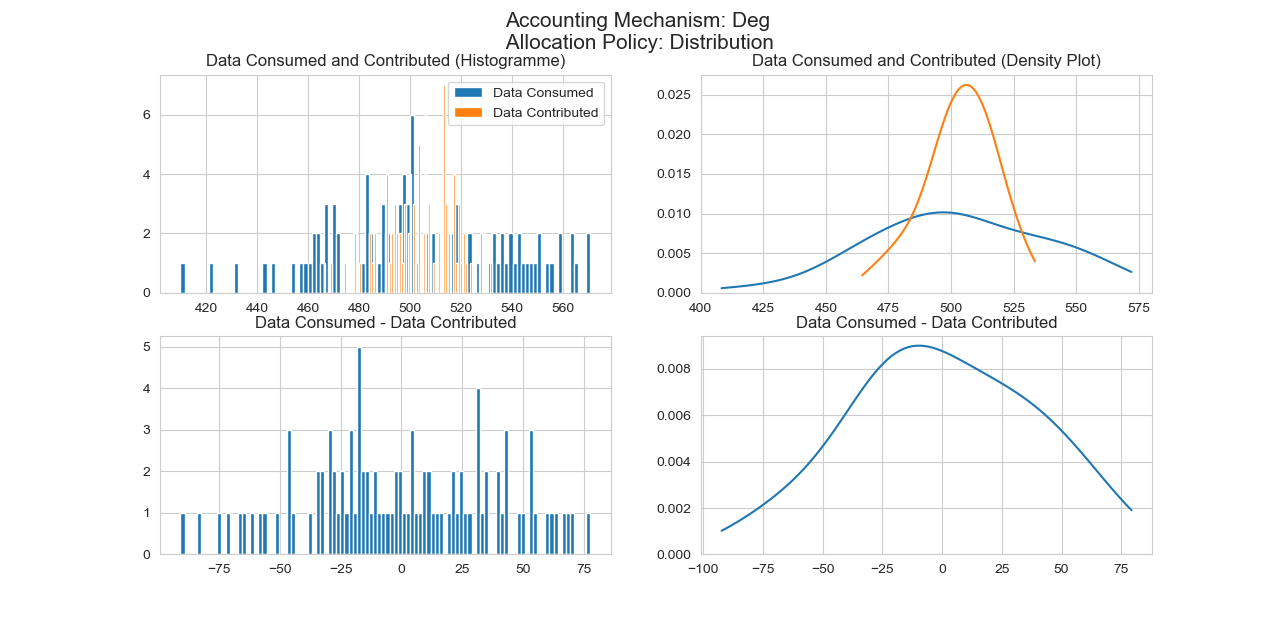
\includegraphics[scale=0.4]{Acc_Deg_Dist.png}
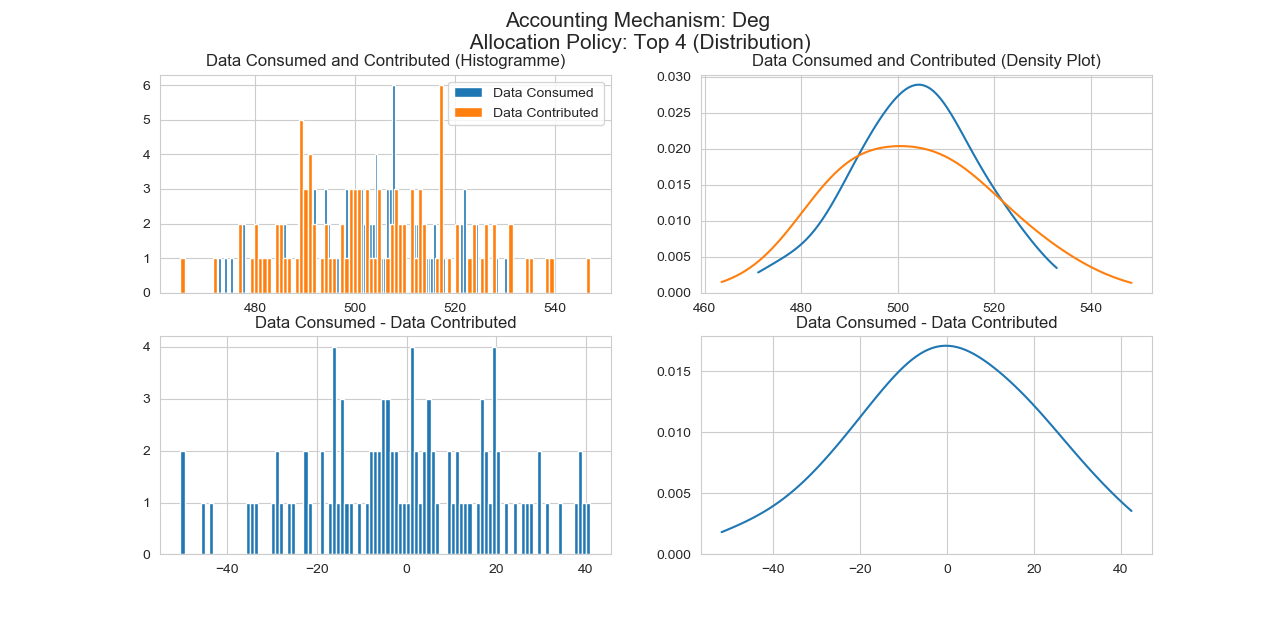
\includegraphics[scale=0.4]{Acc_Deg_Top_4_Dist.png}
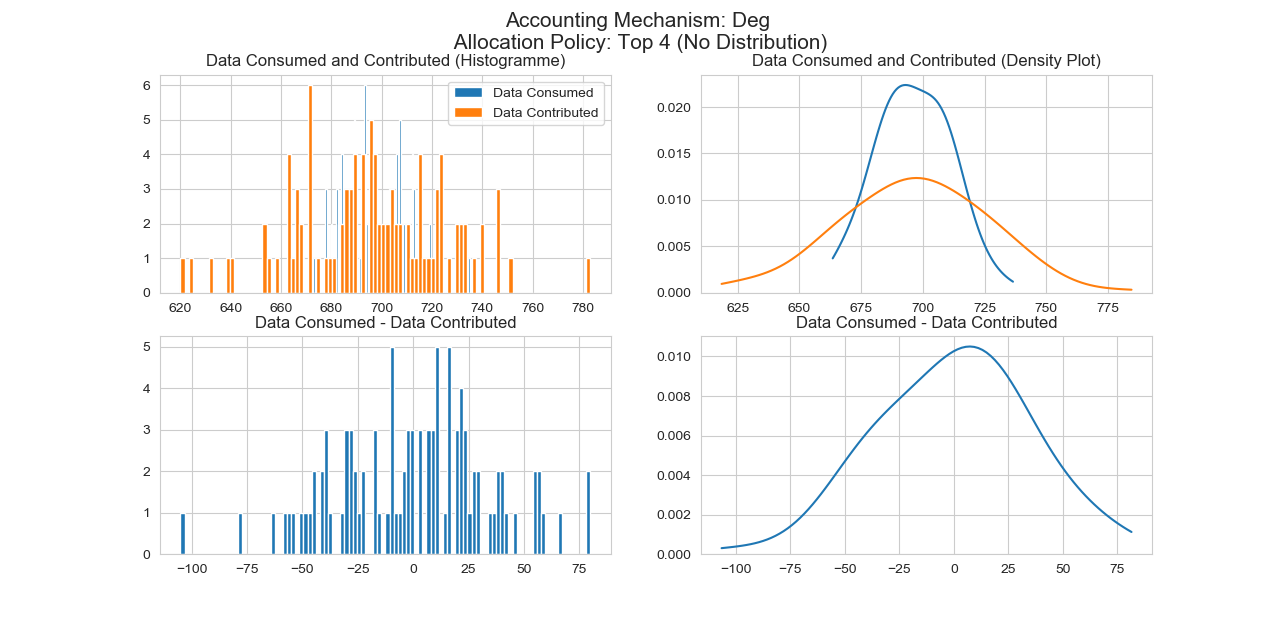
\includegraphics[scale=0.4]{Acc_Deg_Top_4_No_Dist.png}
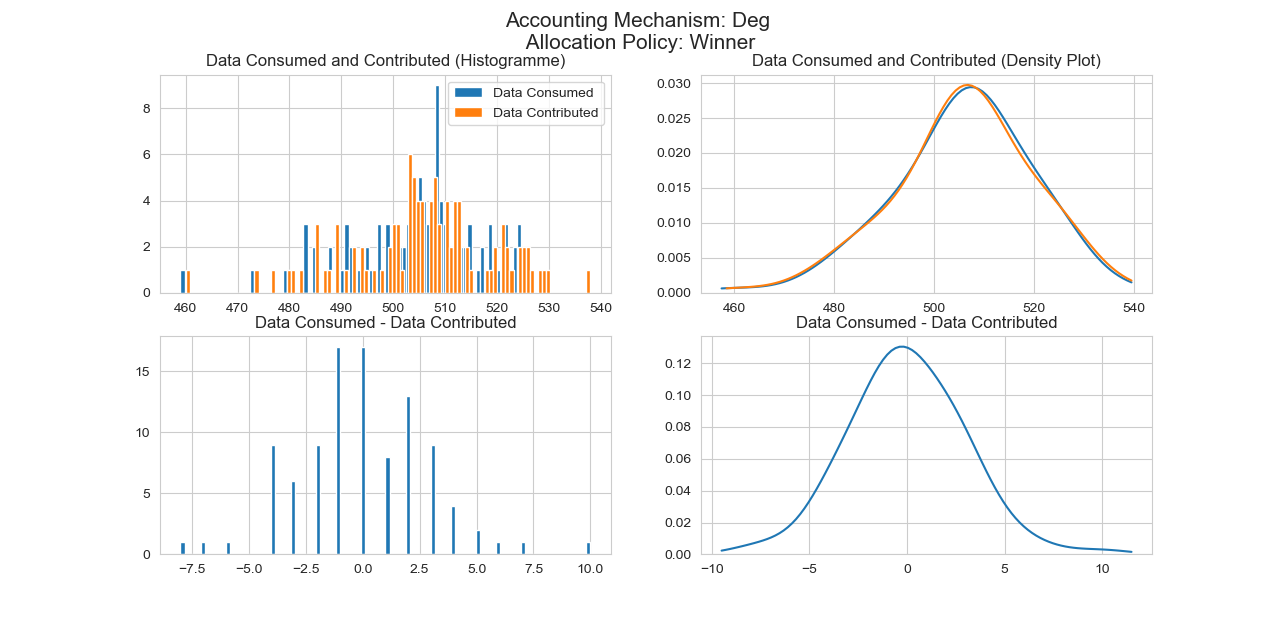
\includegraphics[scale=0.4]{Acc_Deg_Winner.png}
\end{center}
\end{figure}

\begin{figure}[H]
\begin{center}
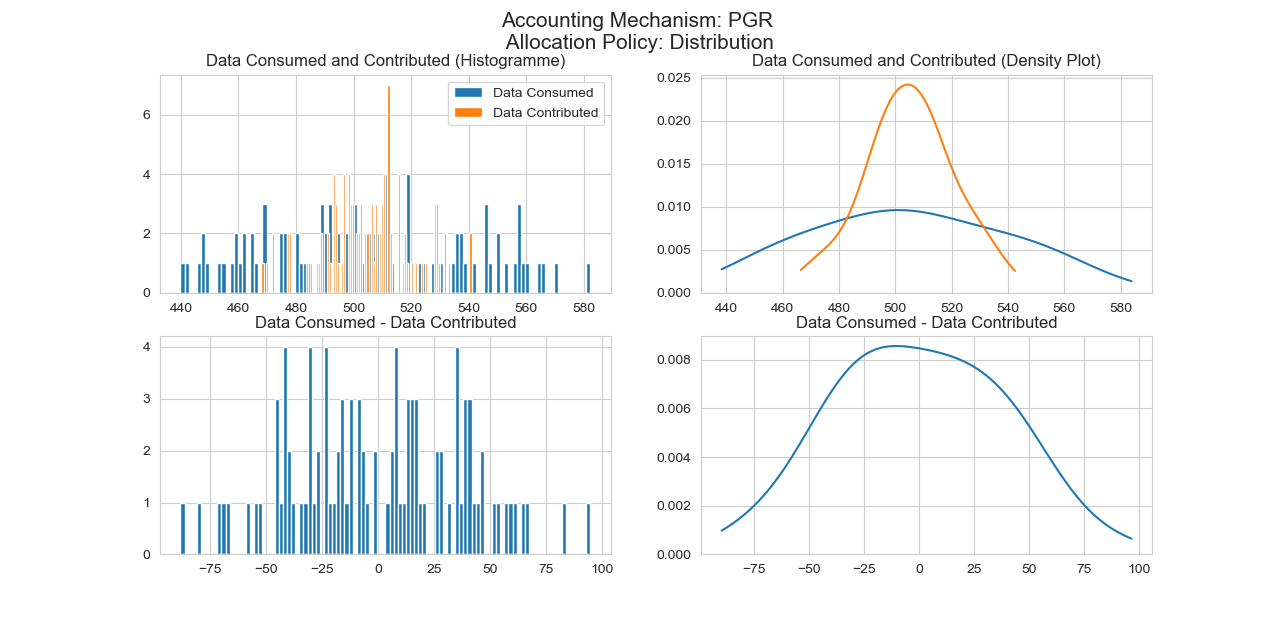
\includegraphics[scale=0.4]{Acc_PGR_Dist.png}
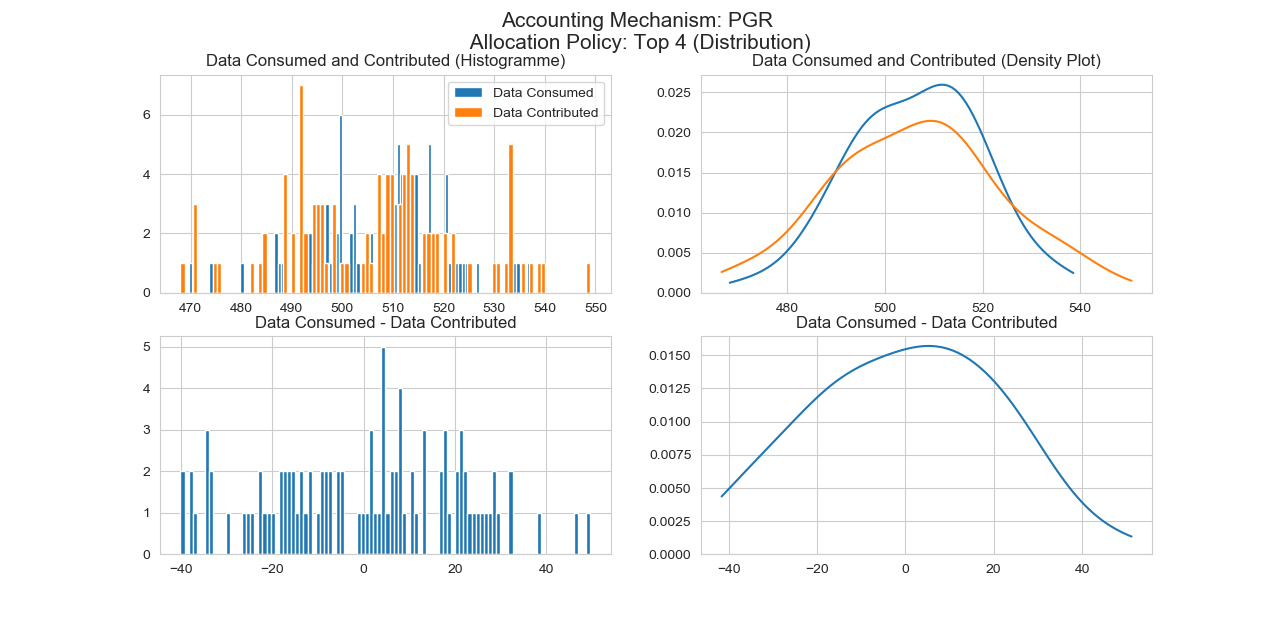
\includegraphics[scale=0.4]{Acc_PGR_Top_4_Dist.png}
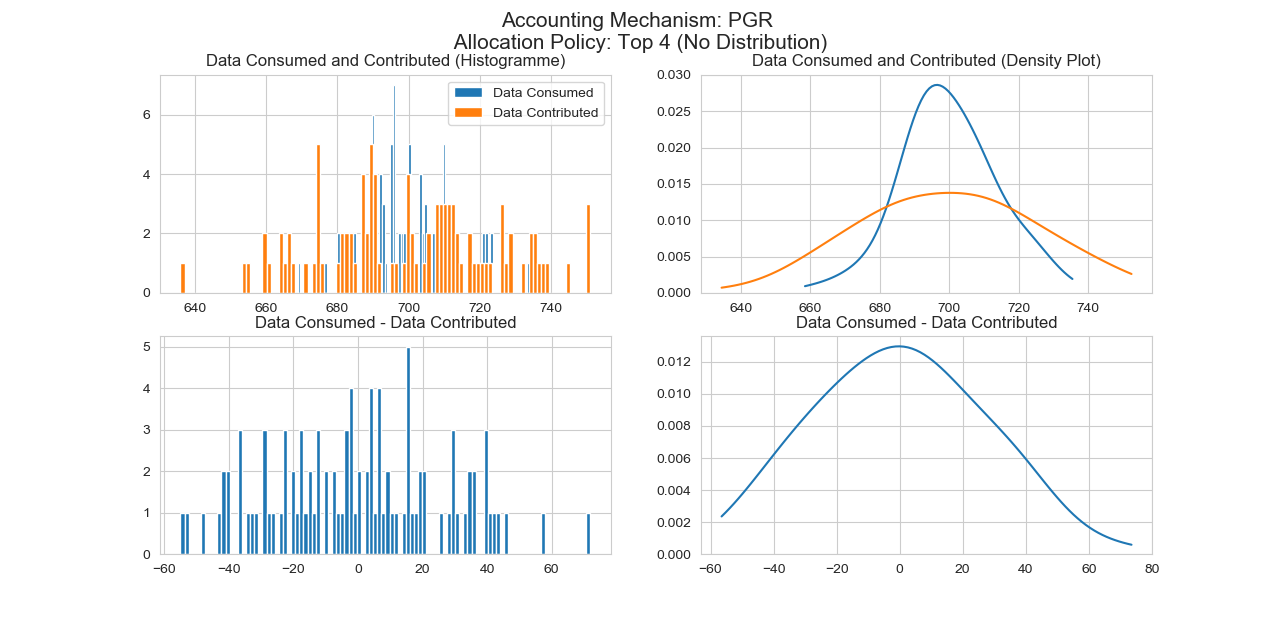
\includegraphics[scale=0.4]{Acc_PGR_Top_4_No_Dist.png}
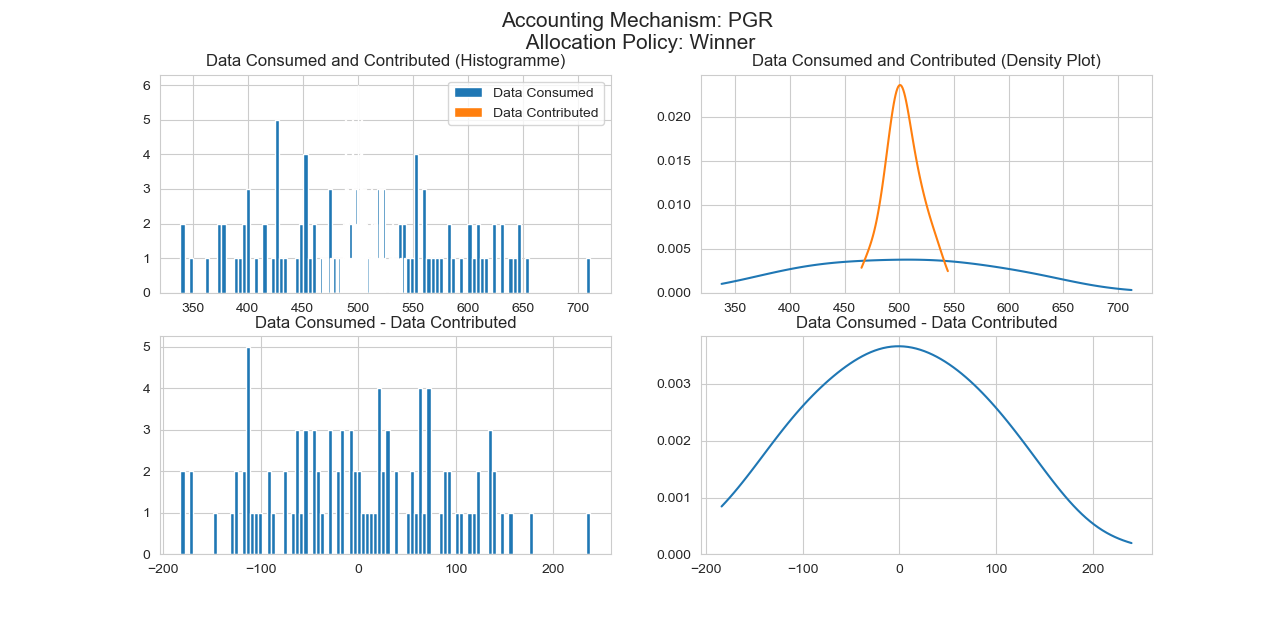
\includegraphics[scale=0.4]{Acc_PGR_Winner.png}
\end{center}
\end{figure}

\noindent{}For the simplest accounting mechanism that assigns $0$'s to all nodes in the network, we find that the distribution policy leads to a rather wide-ranging distribution of net contributions made to the network, which entails that the distribution policy (in combination with all $0$'s accounting values) is not very effective in preventing or mitigating lazy freeriding. We can see that after 1000 rounds there are nodes that have net contributions of -100, while others have net contributions of up to 100. Hence the gap between lazy freeriders and cooperators is very large. This however may have to do with the fact that the accounting mechanism does not satisfy positive-report responsiveness and does not decrease for freeriders. \vspace{1em}\\

\noindent{}The top 4 (distribution) policy does a much better job at ensuring a fair distribution in the network, while the top 4 (no distribution) policy is slightly more slanted towards the negative side and the winner-takes-all policy has a slightly heavier tail on the positive side. Hence for this given accounting mechanism we conclude that the top (distribution) policy is most effective at preventing lazy freeriding. A problem here is that the all $0$'s accounting mechanism obviously does not yield different values for different nodes that behave differently and hence no allocation policy can really prevent freeriding given such an accounting mechanism. \vspace{1em}\\

\noindent{}For the degree accounting mechanism we find that the distribution policy again has a large variance and therefore with a mode that lies on the negative side with values ranging from -100 to 75. The top 4 (distribution) policy yields a slightly more fair distribution with values ranging from -40 to 40, while the top 4 (no distribution) policy has a much worse distribution. Finally the winner-takes-all policy yields by far the most narrow distribution and can therefore be deemed the best allocation policy with respect to the degree accounting mechanism.\vspace{1em}\\

\noindent{}In the case of the personalised PageRank accounting mechanism we find that the distribution policy returns a distribution similar to the distributions we saw for different accounting mechanisms. The fact that the distribution policy always returns very similar distributions of data in the network lies in the fact that every node in the choice set is always served and only the amount the it receives varies depending on its accounting value. Seeing however that these values vary, for the most part, only slightly it seems obvious that this allocation policy always returns a very similar distribution. The same holds for the top 4 (distribution policy). Although we do observe some differences between the distributions. These may, however be attributed to the randomness of the simulation.\vspace{1em}\\

\noindent{}We do observe a rather surprising property of the winner-takes-all policy in the case fo the personalised PageRank, namely a very large variance in the distribution, i.e. it is very ineffective in preventing lazy-freeriding. We note that this can be mostly attributed to the personalised PageRank accounting mechanism itself as it is path-based, which means that if a node $j$ leeches from another node $k$ and thereafter queries another node $i$ then $S_j(G_i,C_i)$ is not affected by this leech so long as no path from $j$ to $i$ traverses $k$. This can lead to unpunished freeriding. We conclude this section by noting that there is no allocation policy wich is the best at preventing lazy-freeriding. We note that each accounting mechanism may have a different allocation policy which is best suited for it. \vspace{1em}\\

\noindent{}Note that the choice set $C_i$ is assembled probabilistically, such that every node in the network has the same probability of lying in $C_i$. The attacker does not know $i$'s subjective work graph and therefore there is no strategic way for $j$ to choose which of its sybil nodes queries which node in the network for data. Hence, regardless of which allocation policy is used in the network, $j$ maximises the possible profit, by diversifying the nodes that are queried by $j$ and its sybils, i.e. all sybil nodes should query a different randomly chosen node. It may even seem like the upper inequalities contain the union of independent events, but this is not the case, as they all depend on the same interaction graph. \vspace{1em}\\
 
\noindent{}The fact that the winner-takes-all allocation policy leads to a lower porbability of nodes from the sybil region being served than nodes from the rest of the network, eventhough the distribution policy may be fairer with respect to the distribution of data among network participants, leads us to believe that it is the best one for our simulations. Although it should be stated that the experiments did yield much different results for different accounting mechanisms and depending on the parameters of the model, these results may vary even more from simulation to simulation. \vspace{1em}\\

\noindent{}The trade-off to this however is that it strongly limits the set of nodes that can consume data, to only a few nodes with the highest reputation, which limits the flow of data in the network and consequently its operability or usability. An alternative to this is for the node willing to contribute to split the file into equally sized pieces, which it distributes among the $n$ highest ranking node(s) in its choice set, or possibly an allocation policy that serves all nodes in the choice set with parts of a file, which in size correspond to every node's accounting value, i.e. every $j\in{}C_i$ receives

\[
\tilde{w}\cdot\frac{S^M_j(G_i,C_i)}{\sum\limits_{k\in{}C_i}^{}S^M_k(G_i,C_i)}.
\]

\noindent{}Computing these values becomes increasingly complicated and we therefore confine our model to the winner-takes-all policy, where, in case there are two nodes that both have the highest accounting values, one of the two is randomly chosen to receive some work performed. \vspace{1em}\\

\noindent{}Recall that whether a node $j$ is served by node $i$ depends on the accounting values of all nodes in the choice set $C_i$. Next, we have to assume that there exists some probability distribution of accounting values $\left\lbrace{}S^M_k(G_i,C_i)\,|\,k\in{}V_i\right\rbrace$ for every node $i\in{}V$. This is, of course, highly dependent on the accounting mechanism itself. Let $X_i$ be the random vector of accounting values for all nodes in the work graph from the perspective of node $i$. Then $X_{ik}$ will be the random variable describing the accounting value assigned to $k$ from the perspective of $i$. Note that we deliberately no longer choose subjective work graph. Every node in the work graph that is not in the subjective work graph of $i$ will simply be assigned an accounting value of 0. We also assume that every node assigns itself an accounting value of 0. Just for simplicity. \vspace{1em}\\ 

\noindent{}We do not know much about this yet as it highly depends on the accounting mechanism that is chosen. However, given the structure of the kind of graph that evolves over time as this process in rounds continues, we find that the distribution in accounting values may converge to some distribution similar to the geometric distribution or the poisson distribution. This distribution could indicate the amount of work a node could consume in the next round. We would assume that if a node finds itself in the p-th percentile of the distribution of accounting values in the network then its likelihood of being served data in the next round is, in expectation, $p\%$. \vspace{1em}\\

\noindent{}We introduce the random variable $X_{ij}=S^M_j(G_i,C_i)$, which is the trust $i$ has in $j$ and define the random vectors $X_i:=(X_{i1},\ldots,X_{in})$ for $i\in{}V$. Then, of course it holds that the probability of node $k$ being the highest ranking node in $i$'s choice set is given by 

\[
\mathbb{P}(X_{ik}>X_{ij}\,\,\textit{f.a. }j\in{}C_i\backslash\lbrace{}j\rbrace) = \mathbb{P}\left(\bigcap\limits_{j\in{}C_i\backslash\lbrace{}k\rbrace}X_{ij}<{}X_{ik}\right)
\]

\noindent{}Now, because $C_i$ is sampled randomly with $\mathbb{P}(j\in{}C_i)=\frac{q}{|V|-1}$ iid for all $j\in{}V$ it follows 

\[
\mathbb{P}(X_{ik}>X_{ij}\,\,\textit{f.a.}\,\,j\in{}C_i) = \mathbb{P}(X_{ik}>X)
\]

\noindent{}where $X$ is the random variable following the distribution of accounting values that the network converges to. \vspace{1em}\\

\noindent{}Now that our model has been established we can return to the original goal of determining $\omega_{+}^{n}$. We define the random variable $Y_{ik}$ as the indicator function which is 1 if $X_{ik}\geq{}X_{ij}$ f.a. $j\in{}V$ and zero else. We then define $G^{(1)}$ as the work graph after the attacker and their sybils have consumed the work they were elligible for after the attack. This continues round for round yielding work graphs $\left(G^{(n)}\right)_{n\in\mathbb{N}}$. Then the expected amount of work node $j$ can consume after sybil attack $\sigma_j^n$ as 

\[
\omega^n_{+}:=\sum\limits_{n\in\mathbb{N}}\tilde{w}^n\cdot\mathbb{E}\left[\sum\limits_{i\in{}V}Y^{(n)}_{ij}+\sum\limits_{l=1}^{n}\sum\limits_{i\in{}V}Y^{(n)}_{is_{jl}}\right].
\]

\noindent{}There is a problem with this definition of sybil attack profit, which stems from the possibility that a node $j$ with $S_j(G_i,C_i)=0$ may still be served by node $i$ in a particular round, if it is the only node in $i$'s choice set. Therefore we find that for any node that queries another node with probability $p$ in every round, the upper sum will be infinite. In order to curb this, we make another assumption of our model. While $V_i$ is obviously always finite, we assume that there are infinite nodes $v$ outside of $i$'s subjective work graph, all with $S^M_u(G_i,C_i)=0$ that will make queries to other nodes following the same paradigm as above. By this logic the choice set $C_i$ will be of infinite size in every round and the probability of $j$ being served in any given round is arbitrarily small. This results in the sum above being finite for any node in the network that does not "cheat". \vspace{1em}\\ 

\noindent{}Note that this sum is impossible to compute for any generic probabilistic setting making it impossible to determine how effective a sybil attack actually is. In order for us to be able to gauge how profitable an attack is, we introduce another pair of definitions of sybil attack rewards, which we denote $\omega_{+}^{n}$(rep) and $\omega_{-}^{n}$(rep). \vspace{1em}\\ 

\noindent{}Recall that the point behind a sybil attack is to artificially increase the value of the accounting values of one or more nodes in the sybil region from the perspective of as many honest nodes as possible. Hence, one might define the reward of such an attack by 

\[
\omega_{+}^{n}(\textit{rep}) = \sum\limits_{i\in{}V'\backslash\left\lbrace{}j,s_{j1}\ldots{}s_{jn}\right\rbrace}\sum\limits_{s\in\left\lbrace{}j,s_{j1}\ldots{}s_{jn}\right\rbrace}S^M_s(G'_i,C'_i)
\]

\noindent{}Strictly speaking the reward of the sybil attack should, in fact be the sum of all accounting values of sybil nodes in the new work graph minus the accounting values of the attacking node $j$ before the attack has been carried out, i.e.

\[
\sum\limits_{i\in{}V'\backslash\left\lbrace{}j,s_{j1}\ldots{}s_{jn}\right\rbrace}\sum\limits_{s\in\left\lbrace{}j,s_{j1}\ldots{}s_{jn}\right\rbrace}S^M_s(G'_i,C'_i) - \sum\limits_{i\in{}V\backslash\left\lbrace{}j\right\rbrace}S^M_j(G_i,C_i)
\]

\noindent{}Naturally, we may define the profit of a sybil attack as the reward divided by the work invested. We now need to define $\omega^{n}_{-}$(rep), which needs to be analogous to the earlier defined $\omega_{-}^{n}$, but in terms of accounting values. The reasoning for the definition of $\omega_{-}^{n}$ above was that we were trying to capture the amount work invested into the network by a sybil attacker. In terms of accounting values, we can define this concept as the aggregated accounting values a sybil attacker has "earned" through their honest work, invested into the network. \vspace{1em}\\

\noindent{}We do this by changing the structure of the graph $G=(V,E,w)$. $G$ was the graph that contained all nodes, including the attacker $j$ without the sybil nodes, before the attack took place. $G':=G\downarrow\sigma^n_j$ was the work graph altered by the sybil attack, with $V'=V\cup{}S$. We now introduce a third graph $G''=(V'',E'',w'')$ where $V''=V$ and $w'':V\times{}V\rightarrow\mathbb{R}$ with $w''(u,v)=w(u,v)$ f.a. $u,v\in{}V\backslash\left\lbrace{}j\right\rbrace$ and $w(j,u)=\sum\limits_{s\in{}S\cup\left\lbrace{}j\right\rbrace}w'(s,u)$. Graphically, this means that we "collapse" all sybil nodes into a single node which we will label $j$ again. This means that all incoming and all outgoing edges from any sybil node into the honest region of the graph, are attached to $j$ in $G''$. \vspace{1em}\\

\begin{figure}[H]
\begin{center}
\includegraphics[scale=0.7]{"Cost Rep(1)".PNG} 
\includegraphics[scale=0.7]{"Cost Rep(2)".PNG} 
\includegraphics[scale=0.7]{"Cost Rep(3)".PNG}
\caption{Example of Collapsing a Sybil Region}
\label{fig:Example of Collapsing a Sybil Region}
\end{center}
\end{figure}

\noindent{}The point is that the aggregate of accounting values that the sybil attacker has gained should be compared to the accounting values that they're actually entitled to based on the actual work performed, i.e. the attack edges. All edges that do not enter or leave the sybil region are therefore disregarded and any increase in reputation that the sybil attackers may gain through the sybil-internal edges is dropped. In formula this would be given by \vspace{1em}\\

\[
\sum\limits_{i\in{}V''\backslash\left\lbrace{}j\right\rbrace{}}S^M_j(G_i'',C_i'')
\]

\noindent{}In summary, we obtain the following definitions of sybil attack costs and rewards 

\begin{align*}
\omega_{+}^{n}(rep) &= \sum\limits_{i\in{}V'\backslash\lbrace{}j,s_1,\ldots,s_n}\sum\limits_{s\in\lbrace{}j,s_1,\ldots,s_n\rbrace}S^M_s(G_i',C_i') - \sum\limits_{i\in{}V\backslash\lbrace{}j\rbrace}S^M_j(G_i,C_i) \\
\omega_{-}^{n}(rep) &= \sum_{i\in{}V''\backslash\lbrace{}j\rbrace}S^M_j(G_i'',C_i'') - \sum\limits_{i\in{}V\backslash\lbrace{}j\rbrace}S_j^M(G_i,C_i) \\
\omega_{+}^{n}(work) &= \sum\limits_{n\in\mathbb{N}}\tilde{\omega}\cdot\mathbb{E}\left[\sum\limits_{i\in{}V'\backslash\lbrace{}j,s_{j1},\ldots,s_{jn}\rbrace}\sum\limits_{l=1}^{n}Y'^{(n)}_{is_{jl}} + Y'^{(n)}_{ij}\right] - \sum\limits_{n\in\mathbb{N}}\tilde{\omega}\cdot\mathbb{E}\left[\sum\limits_{i\in{}V\backslash\lbrace{}j\rbrace}Y^{(n)}_{ij}\right] \\
\omega_{-}^{n}(work) &= \sum\limits_{i\in{}V'\backslash\lbrace{}j,s_{j1},\ldots,s_{jn}\rbrace}\sum\limits_{l=1}^{n}w'(s_{jl},i) + w'(j,i) \,\, - \,\, \sum\limits_{i\in{}V\backslash\lbrace{}j\rbrace}w(j,i) 
\end{align*}

\noindent{}Knowing these definitions of sybil attack reward and cost, we can now define the sybil attack profit more rigorously. \vspace{1em}\\

\noindent{}We then say that a sybil attack $\sigma^n_j$ is
\begin{itemize}
\item[] {\bf Strongly Beneficial} if $\omega^n_{+}>0$ and $\omega^n_{-}=0$ or if $\lim\limits_{n\rightarrow\infty}\frac{\omega^n_{+}}{\omega^n_{-}}=\infty$
\item[] {\bf Weakly Beneficial} if $\omega^n_{+}>0$ and $\omega^n_{-}>0$ and $\exists c>0:\,\,\lim\limits_{n\rightarrow\infty}\frac{\omega^n_{+}}{\omega^n_{-}}\geq{}c$
\end{itemize}
\noindent{}Since we have two definitions for $\omega^n_{+}$ and $\omega^n_{-}$, we must differentiate between strongly and weakly beneficial in terms of accounting values and in terms of work. Naturally, the question arises whether these two are equivalent. This is an important question as it is not feasible for us to determine the former ratio of cost to reward in units of work and therefore have to rely on the definition based on accounting values. However, it is the goal of any p2p filesharing network to ensure that there is no excessive data leakage, i.e. one wants to prevent strongly beneficial sybil attacks in the former definition. What we need is an equivalence between the two, under certain conditions. However, we can come up with examples where the profit defined in terms of work converges to $\infty$, but the ratio of accounting values does not. Inversely, there exists an example of an accounting mechanism, for which there exists a strongly beneficial sybil attack, in terms of the ratio of accounting values, that is not strongly beneficial in terms of the ratio of work. \vspace{1em}\\
\end{definition}


\begin{example}[]\ \\
Let $G=(V,E,w)$ be an arbitrary work graph and $j$ a malicious node launching a sybil attack $\sigma^n_j$. Let every agent in the network have the same accounting mechanism $S^M$, which satisfies 
\[
\sum\limits_{j\in{}V_i}S^M_j(G_i,C_i)=c
\]
for some $c>0$ and any given subjective work graph $G_i$ for all $i\in{}V$. Now, let $G'=G\downarrow\sigma^n_j$ be the work graph after the attack has been carried out. Now, let the accounting mechanism $S^M$ satisfy $\lim\limits_{n\rightarrow\infty}\sum\limits_{k=1}^{n}S^M_{s_{jk}}(G_i,C_i)=c$, where $\left\lbrace{}s_{j1},\ldots,s_{jn}\right\rbrace$ are the sybil nodes created by $j$, for some honest agent $i$. We now find that it obviously holds
\[
\lim\limits_{n\rightarrow\infty}\sum\limits_{k=1}^{n}S^M_{s_{jk}}(G_i,C_i)<\infty
\]
while we assume that in this attack there exist finite attack edges. Hence it follows
\[
\lim\limits_{n\rightarrow\infty}\frac{\omega(rep)^n_{+}}{\omega(rep)^n_{-}}<\infty.
\]
However, as $\sum\limits_{k=1}^{n}S^M_{s_{jk}}(G_i,C_i)=c$ it must follow $\sum\limits_{v\in{}V\backslash{}\left\lbrace{}j,s_{j1},\ldots,s_{jn}\right\rbrace}S^M_{}(G_i,C_i)=0$. And therefore it must follow that $\mathbb{P}(Y_{is_{jk}}=1)=1$ f.a. $k$. Hence, whenever either $j$ or any of its sybil nodes query the honest node $i$ for some work, they must be the highest ranking node in $C_i$ and will therefore be served as much data as they want. It therefore holds
\[
\tilde{\omega}\cdot{}\lim\limits_{n\rightarrow\infty}\sum\limits_{k=1}^{n}Y^{(1)}_{is_{jk}} = \omega(work)^n_{+} = \infty,
\]
i.e. $\lim\limits_{n\rightarrow\infty}\frac{\omega(work)^n_{+}}{\omega(work)^n_{-}}=\infty$. 
\vspace{1em}\\

\noindent{}Such an accounting mechanism could be given by the PageRank algorithm, where a node $j$ attacks the network with one edge connecting it to node $i$ with a large edge and then creates many sybils which benefit from this attack edge. As the number of sybils grows, nodes in the sybil region will obtain an increasingly large proportion of the values. This is known as link spamming. \vspace{1em}\\

\noindent{}We can make this example more specific, by the following graph. 

\begin{figure}[H]
\begin{center}
\includegraphics[scale=0.7]{"Example of Ratio (1)".png}
\caption{Example of Strongly Beneficial Sybil Attack in Terms of Work, but not Reputation}
\label{fig:Example of Strongly Beneficial Sybil Attack in Terms of Work, but not Reputation}
\end{center}
\end{figure}

\noindent{}In this graph, $i$ has the personalised pagerank algorithm as accounting mechanism $S^M$ with a very low reset probability $(\leq{}0.0001)$. $j$ launches a sybil attack with 3 nodes and $k$ is an honest node, having performed 5 units of work for $i$. $j$ performs the same amount of work for $i$ as an attack edge and then creates fake edges, connecting the sybils. These edges must have extremely high weights, in order for the sybil attack to be as effective as possible. Now, if $i$ computes the personalised pagerank scores for all nodes in its subjective work graph we find that $j$ and its sybil nodes have much higher reputation values than $k$. In this particular example it would be 
\[
k:10^{-5}, j:0,29, s_{j1}:0,14, s_{j2}:0,29, s_{j3}:0,29.
\]
Hence, it obviously holds $\frac{\omega^3_{+}(rep)}{\omega^3_{-}(rep)} = 4 < \infty$ \vspace{1em}\\

\noindent{}Now, we want to compute $\frac{\omega^3_{+}(work)}{\omega^3_{-}(work)}$ and we will show that this is infinite. Let $s_{j1}$ now query some data from node $i$. It is guaranteed that $s_{j1}$ is the highest ranking node in $i$'s subjective work graph and will therefore be served some amount of data $X(=5)$, which changes the work graph into the one below. 

\begin{figure}[H]
\begin{center}
\includegraphics[scale=0.7]{"Example of Ratio (2)".png}
\caption{Example of Strongly Beneficial Sybil Attack in Terms of Work, but not Reputation}
\label{fig:Example of Strongly Beneficial Sybil Attack in Terms of Work, but not Reputation (2)}
\end{center}
\end{figure}

\noindent{}It now obviously holds $\omega^3_{+}(work) = \tilde{\omega}\cdot{}\mathbb{E}[Y_{is_{j1}}]=5$ and $\omega^3_{+}(work)=5$. However, seeing as the weights of the fake edges are meant to be extremely high, $s_{j1}$'s leech of 5 units of work barely affects the pagerank values at all. We obtain the new accounting values
\[
k:0,0001, j:0,286, s_{j1}:0,142, s_{j2}:0,0286, s_{j3}:0,286
\]

\noindent{}Hence, it follows $\mathbb{P}(Y^{(2)}_{is_j1}=1)=1$ and this continues for an arbitrarily long sequence of rounds. If at some point point the weight $w_i(s_{j1},i)$ becomes so large that it begins to affect the accounting values of the other sybils, then $j$ simply increases the weight of the fake edges again, and this game continues forever. Hence, we find that 
\[
\frac{\omega^3_{+}(work)}{\omega^3_{-}(work)}=\infty
\]
\end{example}

\noindent{}The example above is a case of a strongly beneficial sybil attack. However, it should be noted that, the attacker in this example can only leech excessively from a single node $i$. If another node $k$ were to be created that receives some work from $i$, then it would also be susceptible to the high reputation of the attacker $j$ and its sybils. However the effect of the sybil attack would be bounded by the weight $w(i,k)$. (Provided we assume weak transitive trust). Therefore it would be unlikely that the attackers could leech anywhere near as much from $k$ as they could leech from $i$. \vspace{1em}\\

\noindent{}The effectiveness of this attack is limited to node $i$, which is certainly problematic for a P2P network, but not as much as a sybil attack, through which the attacker could leech arbitrary amounts from several nodes (possibly even a significant proportion of the network). In fact, the upper example may not even qualify as a proper sybil attack. Instead this type of attack is often also referred to as an {\it Eclipse Attack}. Note that a strongly beneficial eclipse attack is not nearly as severe as a strongly beneficial sybil attack. In fact, a strongly beneficial eclipse attack may be less problematic than some types of weakly beneficial sybil attacks. This prompts us to introduce a new definition.\vspace{1em}\\

\noindent{}Next, we introduce an example in which an attacker can accummulate large accounting values without necessarily gaining infinite work from it.

\begin{example}[]\ \\
Let $S^M_k(G_i,C_i)$ be the accounting mechanism given by the number of shortest paths from $i$ to every other node in the network that traverse node $k$. Let $(SP^i_v)_{v\in{}V_i\backslash{}\left\lbrace{}i\right\rbrace}$ be the shortest paths connecting $i$ and node $v\in{}V_i$. Now let 
\[
X_{ij}=\sum\limits_{v\in{}V_i\backslash\left\lbrace{}i\right\rbrace}1_{\left\lbrace{}j\in{}\,SP^i_v\right\rbrace}
\]

\noindent{}Given an arbitrary work graph $G=(V,E,w)$ a node $j$ may decide to launch a sybil attack such that $G'=G\downarrow\sigma^n_j$ with one attack edge connecting to another agent $i$ and creating a large number of sybil nodes that all do some work for $j$. Consequently, node $j$ will obtain the accounting value from the perspective of $i$ 

\[
X_{ij}=\sum\limits_{v\in{}V_i\backslash\left\lbrace{}i\right\rbrace}1_{\left\lbrace{}j\in{}\,SP^i_v\right\rbrace} \geq \sum\limits_{k=1}^{n}1_{\left\lbrace{}j\in{}\,SP^i_{s_{jk}}\right\rbrace} = n
\]

\noindent{}Obviously, it then holds $\lim\limits_{n\rightarrow\infty}\sum\limits_{k=1}^{n}S^M_{s_{jk}}(G_i,C_i)=\infty$ while the amount of work that was put in, is bounded by the single attack edge. And therefore it is $\lim\limits_{n\rightarrow\infty}\frac{\omega(rep)^n_{+}}{\omega(rep)^n_{-}}=\infty.$ \vspace{1em}\\

\noindent{}However, this does not imply that node $j$ will have the highest (or one of the highest) reputations in the network. As a matter of fact node $i$ itself will have a reputation that is at least as high as node $j$, this is because any path that traverses $j$ must also traverse $i$, as $j$ only has one attack edge. Hence $i$ will have a reputation just as high as $j$. This may hold for many other nodes in the network as well and therefore the likelihood of node $j$ being the highest ranking node in any other agent's choice set is not significantly close to 1. Hence it may follow $\lim\limits_{n\rightarrow\infty}\frac{\omega(work)^n_{+}}{\omega(work)^n_{-}}<\infty$.
\end{example}

\noindent{}This is rather problematic as we want to prevent the former, while only being able to determine the latter. We want to find some restrictions under which the upper two concepts become equivalent. Or, if this is not possible, we would like to find some restrictions on accounting mechanisms that make the latter stronger than the fomer. By this we mean that if a sybil attack is strongly beneficial in terms of reputation it must also be strongly beneficial in terms of work. Hence, we could find that an accounting mechanism that resistant to strongly beneficial sybil attacks in term of reputation must also be resistant to them in terms of work. We call this property of accounting mechanisms representativeness. \vspace{1em}\\

\begin{definition}[Representative]\ \\
\noindent{}We say an accounting mechanism $S^M$ is {\it weakly representative} if it holds \vspace{1em}\\

\[
\lim\limits_{n\rightarrow\infty}\frac{\omega^n_{+}(rep)}{\omega^n_{-}(rep)}<\infty\,\, \Longrightarrow \,\,\lim\limits_{n\rightarrow\infty}\frac{\omega^n_{+}(work)}{\omega^n_{-}(work)}<\infty \quad\textit{for all sybil attacks }(\sigma_j^n)_{n\in\mathbb{N}}
\]

\noindent{}Subsequently, we call an accounting mechanism $S^M$ {\it strongly representative} if it holds \vspace{1em}\\

\[
\lim\limits_{n\rightarrow\infty}\frac{\omega^n_{+}(rep)}{\omega^n_{-}(rep)}<\infty\,\, \Longleftrightarrow  \,\,\lim\limits_{n\rightarrow\infty}\frac{\omega^n_{+}(work)}{\omega^n_{-}(work)}<\infty \quad\textit{for all sybil attacks }(\sigma_j^n)_{n\in\mathbb{N}}
\]

\end{definition}

\noindent{}The question now arises, what requirements $S^M$ must satsify, in order for it to be weakly and/or strongly representative. We claim that in order for the upper inequality (weak representativeness) to be true there must exist some function $f$ such that \vspace{1em}\\

\[
f_{S^M}\left(\frac{\omega^{n}_{+}(rep)}{\omega^{n}_{-}(rep)}\right) = \frac{\omega^{n}_{+}(work)}{\omega^{n}_{-}(work)} \vspace{1em}\\
\]

\noindent{}where $f_{S^M}:\mathbb{R}_{\geq{}0}\rightarrow\mathbb{R}_{\geq{}0}$ should be nondecreasing and well-defined, i.e. $f_{S^M}(x)<\infty$ f.a. $x<\infty$. Additionally, for strong representativeness to be satisfied, $f_{S^M}$ needs to satisfy $\lim\limits_{x\rightarrow\infty}f_{S^M}(x)=\infty$. This is a problem that has been widely disregarded in the literature so far, such as in \cite{A Random Walk Based Trust Ranking in Distributed Systems}. So far the effectiveness of sybil attacks has only been researched for generic defintions of $\omega_{+}^{n}$ and $\omega_{-}^{n}$, \cite{On the Sybil-Proofness of Accounting Mechanisms}. However, at closer inspection, we find that a more rigorous definition of these values is indeed required. \vspace{1em}\\ 

\noindent{}If for a given accounting mechanism $S^M$ we know that such a function exists, then we can guarantee that a sybil attack which is strongly beneficial in terms of accounting values is, in fact, strongly beneficial in terms of the work the attacker can leech as well. Conversely, we know that if an accounting mechanism is resistant to strongly beneficial sybil attacks in terms of accounting values then it is actually resistant to sybil attacks. \vspace{1em}\\

\noindent{}Now note that for any arbitrary accounting mechanism it must already hold

\[
\omega_{-}^{n}(work)=0 \,\,\Longrightarrow \,\, \omega_{-}^{n}(rep)=0,
\]

\noindent{}This is because any sybil attack with $\omega_{-}^{n}(work)=0$ cannot have any additional attack edges, i.e. all edges added to the work graph by the attacker will be within the sybil region $S$ and not connected to any outside nodes. From this we can conclude that 

\[
\frac{1}{\omega_{-}^{n}(work)} = \infty \,\, \Longrightarrow \,\, \frac{1}{\omega_{-}^{n}(rep)} = \infty
\]

\noindent{}and obviously

\[
\frac{1}{\omega_{-}^{n}(rep)} < \infty \,\, \Longrightarrow \,\, \frac{1}{\omega_{-}^{n}(work)} < \infty
\]

\noindent{}and therefore we can conclude that a function $f_{S^M}$ mapping 

\[
f_{S^M}(\omega^n_{+}(rep)) = \omega^n_{+}(work)
\]

\noindent{}with the same properties as mentioned above, suffices to ensure weak and strong representativeness. This $f_{S^M}$ then denotes the maximum amount of data a set of nodes with a given aggregate of reputation values could leech without making any contributions anymore after the initial $\omega_{-}^{n}(work)$. If for a given accounting mechanism $S^M$ we find that $f_{S^M}$ is not well-defined then we conclude the given $S^M$ is an inappropriate choice of accounting mechanism as it is not representative.\vspace{1em}\\

\noindent{}An obiouvs problem arises from this definition of $\omega_{+}^{n}(rep)$, namely the fact that we do not take into account that the accounting values obtained through the sybil attack might be distributed over the number of sybil identities, as opposed to all being attributed to the main attacking node $j$. This may lead to sybil attacks which are very beneficial in terms of accounting values, but not at all in terms of the work that can be consumed. The following example represents this well.

\begin{example}[]\ \\
Let $G=(V,E,w)$ be a work graph with honest node $i$ and attacker $j$. Let $j$ launch a sybil attack $\sigma^n$ with $n$ sybil identities $s_{j1},\ldots,s_{jn}$ and let $S^M()$ be the BarterCast accounting mechanism given by the maxflow algorithm. \cite{Bartercast: A Practical Approach to Prevent Lazy Freeriding in P2P Networks}. Let $G'$ be the work graph after the sybil attack, given by 

\begin{figure}[H]
\begin{center}
\includegraphics[scale=0.7]{"Sybil Attack on BarterCast".PNG}
\caption{Sybil Attack on BarterCast}
\label{fig:Sybil Attack on BarterCast}
\end{center}
\end{figure} 

\noindent{}In this example, we obtain the values $\omega_{-}^{n}(rep)=1$ and $\omega_{+}^{n}(rep)=n$, which implies $\lim\limits_{n\rightarrow\infty}\frac{\omega_{+}^{n}(rep)}{\omega_{-}^{n}(rep)}=\infty$. However, we find that $S^M_{is_{jk}}=1$ f.a. $k=1,\ldots,n$ and because it holds $S^M_k(G_i,C_i)=3$, it is obvious that if $i$'s allocation policy is winner-takes-all, $\omega^{n}_{+}(work)=0$.
\end{example}

\noindent{}From this we can conclude that its impossible for us to explicitly determine a function $f^{S^M}$ for any accounting mechanism in an arbitrary work graph with an undefined sybil attack. While it may not be practically applicable it does hold significant theoretical weight with respect to identifying strongly beneficial sybil attacks and/or sybil-proof accounting mechanisms. The main conclusion from this chapter can be summarised as follows. \vspace{1em}\\ 

\begin{corollary}[]\ \\
\noindent{}If an accounting mechanisms $S^M$ does not allow for a strongly beneficial sybil attack $\sigma_j^n$ with respect to accounting values to exist, i.e.

\[
\forall\left(\sigma_j^n\right)_{n\in\mathbb{N}}:\lim\limits_{n\rightarrow\infty}\frac{\omega^{n}_{+}(rep)}{\omega^{n}_{-}(rep)}<\infty
\]

\noindent{}and is (at least) weakly representative, then we find that it does not allow for any strongly beneficial sybil attacks in terms of work, i.e.

\[
\forall\left(\sigma_j^n\right)_{n\in\mathbb{N}}:\lim\limits_{n\rightarrow\infty}\frac{\omega^{n}_{+}(work)}{\omega^{n}_{-}(work)}<\infty
\]
\end{corollary}
 
\noindent{}Hence, an ideal accounting mechanisms would satisfy the upper two properties.

\begin{comment}
\subsection{Utility of Trust/Reputation, etc}
\label{subsec:Utility of Trust/Reputation}
\begin{center} [Check Bram van den Heuvel's Trust in Distributed Systems (chapter 3) for this]\vspace{1em}\\ \end{center}
Naturally, agents must perform work in order to obtain a high value in a the accounting mechanism so they can have work be done for them, thus the question of utility arises what increase in reputation corresponds to (in terms of utility) one unit of work performed. We introduce 3 separate utility functions for each agent $i$: $u_i^W$, $u_i^V$ and $u_i^M$. Here $u_i^W(k)$ determines the utility of performing $k$ units of  work for another agent (this will always be negative), $u_i^V(k)$ denotes the utility derived from obtaining $k$ units of work from another agent, and $u_i^M(r)$ represents the utility of having $S^M_i(G_j)=r_j$ for $r\in\mathbb{R}^{n-1}$, which of course, is nondecreasing in $\mathbb{R}_{\geq{}0}$. The utility of the reputation of an agent is a weighted sum of the utility that this agent obtains from having a certain reputation/accounting value with one of its peers $j$, i.e. $u_i^M(r_1,\ldots,r_{i-1},r_{i+1},\ldots,r_n)=\sum\limits_{j\neq{}i}^{}\alpha_j\cdot{}u_{ij}^M(r_j)$ where $\alpha_j\in[0,1]$ and $\sum\limits_{j\neq{}i}\alpha_j=1$.\vspace{1em}\\

\noindent{} The other two utility functions are given by $u_i^W:D\rightarrow{}\mathbb{R}_{\leq{}0}$ and $u_i^V:D\rightarrow{}\mathbb{R}_{\geq{}0}$ where $D$ is the set of possible up-/download sizes, i.e bandwidth.

\noindent{} $u_{ij}^M(r_j)$ must be defined recursively depending on the global reputation of $j$. This captures the transitivity of trust we are trying to achieve. How exactly we will do this remains open.\vspace{1em}\\

\noindent{} Now, if some agent $j$ approaches agent $i$ requesting $d$ data, agent $i$ will go through with the transaction if the following inequality is satisfied:
If $i$ has reputation values $(r_1,\ldots,r_{i-1},r_{i+1},\ldots,r_n)$ before the transaction transpires and $(r'_1,\ldots,r'_{i-1},r'_{i+1},\ldots,r'_n)$ 
\[
u_i^W(d)+u_i^M(r'_1,\ldots,r'_{i-1},r'_{i+1},\ldots,r'_n) \geq u_i^M(r_1,\ldots,r_{i-1},r_{i+1},\ldots,r_n)
\]
Vice versa, if $i$ needs some file of size $d$ and $j$ is willing to provide it to $i$ whereby $i$ loses some reputation through the transaction, i.e. from $(r_1,\ldots,r_{i-1},r_{i+1},\ldots,r_n)$ to $(r'_1,\ldots,r'_{i-1},r'_{i+1},\ldots,r'_n)$, then $i$ will go through with the transaction if
\[
u_i^V(d)+u_i^M(r'_1,\ldots,r'_{i-1},r'_{i+1},\ldots,r'_n) \geq u_i^M(r_1,\ldots,r_{i-1},r_{i+1},\ldots,r_n)
\]
\end{comment}

\section{Requirements for Accounting Mechanisms}
\label{sec:Requirements for Accounting Mechanisms}
Recall that our overarching goal was to investigate the resistance of accounting mechanisms against strongly beneficial sybil attacks, in terms of work, of course. In this section we will exactly define the kind of resistance we are looking for in a ranking algorithm, i.e. accounting mechanism and analyse some of the requirements accounting mechanisms must satisfy in order to be resistant to such attacks. We begin by introducing definitions of misreport-proof as well as sybil-proof.

\begin{definition}[Misreport-proof]\ \\
Let $G_i$ be the subjective work graph of agent $i$ and let $G_i'$ be the subjective work graph of $i$ after a misreport attack from agent $j$. We say the accounting mechanism $S^M$ of agent $i$ is misreport-proof if for any given choice set $C_i$ of $i$ with $j\in{}C_i$ the two conditions below hold true.
\begin{itemize}
\item $S^M_j(G_i',C_i)\leq{}S^M_j(G_i,C_i)$
\item $S^M_k(G_i',C_i)\geq{}S^M_k(G_i,C_i)$ f.a. $k\in{}C_i\backslash{}\left\lbrace{}j\right\rbrace$
\end{itemize}
\end{definition}
\noindent{}There is a very simple method to make any given accounting mechanisms misreport-proof, it is called the Drop-Edge mechanism, which we will illustrate a little bit later \cite{Accounting Mechanisms for Distributed Work Systems}. This means that we no longer need to lend much weight to the misreport-proofness of accounting mechanisms. Note that Drop-Edge is not an accounting mechanisms itself, it is more a method to enhance any accounting mechanism. Another mechanism to enforce misreport relience for any given accounting mechanism is given by the trustchain architecture \cite{TrustChain: A Sybil-resistant scalable blockchain}. This is a protocol applied on the transaction sets of all agents in the network, ensuring that no misreport can take place without going unpunished. Knowing of these two mechanisms ensures that any accounting mechanism we examine in here can be assumed to be misreport-proof by default. Unfortunately, such a method does not exist (yet) for Sybil resistance. Next, we define the concept of Sybil-proofness. \vspace{1em}\\

\begin{definition}[Sybil-Proofness]\ \\
Given a subjective work graph $G_i$ of agent $i$, we say that the accounting mechanism $S^M$ of $i$ is
\begin{itemize}
\item {\bf sybil-proof against strongly beneficial sybil attacks} if 
\[
\forall{}j\in{}V_i\backslash{}\left\lbrace{}i\right\rbrace \forall (\sigma^n_j)_{n\in\mathbb{N}}\,\exists{}c>0:\,\,\lim\limits_{n\rightarrow\infty}\frac{\omega^n_{+}}{\omega^n_{-}}\leq{}c
\]
\item {\bf sybil-proof against weakly beneficial sybil attacks} if 
\[
\forall{}j\in{}V_i\backslash{}\left\lbrace{}i\right\rbrace \forall (\sigma^n_j)_{n\in\mathbb{N}}:\,\,\lim\limits_{n\in\mathbb{N}}\frac{\omega^n_{+}}{\omega^n_{-}}=0.
\]
\end{itemize}
\end{definition}

\noindent{}Note that sybil-proofness against weakly beneficial attacks is extremely restrictive and very hard to obtain by any form of accounting mechanism, while sybil-proofness against strongly beneficial attacks is easier to achieve and by our standards sufficient for the maintainance of a (mostly) cooperative, functioning network. The reason for this is that while an attacker can launch a sybil attack that returns a multiple of its investment, the idea is that in order for an attacker to leach infinite data, they also have to share infinite data. This means that any form of sybil attack will require some input into the network. No attacker can simply demand all resources in the network,leading to a complete shutdown. Instead, a weakly beneficial sybil attack still stimulates a network enough to maintain its existence. \vspace{1em}\\

\noindent{}Trivially, we want an accounting mechanism to reward contributions while penalising consumption, hence ideally every accounting mechanism should satisfy the following requirement.

\begin{definition}[Positive Report Responsiveness]\ \\
Given a subjective work graph $G_i=(V_i,E_i,w_i)$ derived from a transaction set $TS$ and agent $j$ with transaction set $TS_j$ of length $n$. If $j$ has another interaction $t^j_{n+1}=(k,r)$ with $w>0$ then $TS_j'=TS_j\cup\left\lbrace{}t^j_{n+1}\right\rbrace$ and if the new edge $w(j,k)'=w(j,k)+r$ is in $i$'s agent information set $H_r(i)$ then for the new subjective work graph $G_i'=(V_i,E'_i,w_i')$ it must hold
\[
S^M_j(G_i',C_i')\geq{}S^M_j(G_i,C_i)
\]
and
\[
S^M_k(G_i',C_i')\leq{}S^M_k(G_i,C_i)
\]
\end{definition}

\noindent{}Note however that the upper inequalities may very well be equalities, depending on the algorithm $M$ and the size of the contribution as well as the "distance" between $i$ and $j,k$. They must however not be inverted, i.e. a positive transaction by a node can only increase its reputation and a negative transaction can only do the opposite. The point is that we want our algorithm to reward positive interactions, but not those within a sybil region. This makes the problem at hand an incredibly complicated problem to solve. Some edges should affect trust scores quite strongly, while others should not at all or at least minimally. \vspace{1em}\\

\noindent{}The upper definition can be turned around to "negative report responsiveness". This means that any node that consumes some data, must have a lower reputation value after the interaction than before. Again, this reputation value needn't be strictly lower, it can also be equal. Whether the upper inequalites are in fact hard inequalities plays a very important role in the question of sybil resistance.\vspace{1em}\\ 

\begin{definition}[Path-responsiveness]\ \\
Given a subjective work graph $G_i=(V_i,E_i,w_i)$ we say that an accounting mechanism $S^M$ satisfies path-responsiveness if it holds
\[
S^M_k(G_i,C_i)>0\Rightarrow\exists{}j_1,\ldots,l_n\in{}V_i:\,w_i(j_1,i),w_i(j_n,j_{n-1}),w_i(k,j_n)>0
\]
\end{definition}
\noindent{}This means that in order for a node $k$ to have a positive value in the accounting mechanism from the perspective of another node $i$ there needs to exist at least one path connecting $i$ and $k$. This path needs to correspond to work indirectly performed by $k$ for $i$ through the other nodes in the path. \vspace{1em}\\

\noindent{}Analogously, it must hold
\[
S^M_k(G_i,C_i)<0\Rightarrow\exists{}j_1,\ldots,l_n\in{}V_i:\,w_i(i,j_1),w_i(j_{n-1},j_n),w_i(k,j_n)>0
\]

\noindent{}This is a rather important definition for the following theorems. It is useful as it limits the effect that work performed by nodes that have not performed any work (indirectly) to $i$. This bounds the impact that counterfeit work performed by sybils for other sybils has and will come in handy later. \vspace{1em}\\

\noindent{}We extend this definition to cover several paths as well, which will provide a key stepping stone in the progression of this thesis. 

\begin{definition}[Multiple-path Response Bound]
Let $G_i$ be a subjective work graph from the perspective of node $i$ with several paths $(P_n)_{n\leq{}N}$ connecting $i$ and $k$, as defined above, then the value of $S^M_k(G_i,C_i)$ should be bounded by $\sum\limits_{n=1}^{N}S^M_{k_n}(G'_i,C'_i)$, where $G'_i$ is an altered version of the subjective work graph of $i$, whereby the agent $k$ is "split" into several agents $k_{1},\ldots,k_{N}$, where every $k_j$ is connected to $i$ by exactly one path. \vspace{1em}\\

\noindent{}$G'_i$ is created by splitting the node $k$ into as many nodes as there are paths connecting to it, i.e. $k_1,\ldots,k_N$. Now remove all nodes and edges that are part of any of the paths $P_2,ldots,P_N$. This means, we only keep edges and nodes that are either part of the first path, or that are not in any of the paths at all. We now relabel $k$ (as the end-point of $P_1$), $k_1$. Next, we add path $P_2$ to the graph. Any node $j$ (or edge $e$) in $P_2$ that is also part of $P_1$, is now duplicated into $j_1$ and $j_2$ such that $j_1\in{}P_1$ and $j_2\in{}P_2$ $(e_1\in{}P_1$ and $e_2\in{}P_2)$. We continue this for all paths $P_1,\ldots,P_N$ and obtain $G'_i$. 
\end{definition}

\begin{figure}[H]
\begin{center}
\includegraphics[scale=0.7]{"Path-Responsiveness (1)".png}
\caption{Example of Path-Responsive Work Graph}
\label{fig:Example of Path-Responsive Work Graph}
\end{center}
\end{figure}

\noindent{}This may at first seem like a rather restrictive assumption that eliminates many of the common accounting mechanisms. However, we find that this is in fact not true. The upper definition is satisfied all accounting mechanisms defined in \cite{Hybrid Transitive Trust Mechanisms} Instead, we provide an intuition for why this actually makes sense. In order for an accounting mechanism to determine the trustworthiness of another node, it needs to evaluate this node's contributions and leeches to and from the network. As there is always the possibility of faking edges, we want to limit the effect that edges, which are in between unknown nodes and only take into account the contributions made to nodes that $i$ has at least an indirect connection to. This means we want to evaluate each node $j$ by the outgoing edges that "face" $i$. Each path connecting $j$ to $i$ can be considered an indirect contribution and therefore should influence the accounting value of $j$ in $i$'s subjective work graph. \vspace{1em}\\

\noindent{}However, it is crucial that the effect of an additional path in the network should not exceed the effect that this additional path would have on $S^M_k(G_i,C_i)$ if it were the only path connecting $j$ to $j$. We feel like this is a fairly intuitive and sensible definition. \vspace{1em}\\

\begin{figure}[H]
\begin{center}
\includegraphics[scale=0.5]{"Path-Responsiveness (2)".png}
\caption{Example of another Path-Responsive Work Graph}
\label{fig:Example of another Path-Responsive Work Graph}
\end{center}
\end{figure}

\noindent{}This definition is very closely related to the concept of transitive trust (or transitive accounting values). Transitive trust describes the concept that if a node $i$ trusts another node $j$, and $j$ trusts another node $k$ then it must already follow that $i$ has some trust in node $k$ as well, i.e. 
\[
S^M_j(G_i,C_i)>0\,\,\&\,\,S^M_k(G_j,C_j)>0\,\,\Rightarrow\,\,S^M_k(G_i,C_i)>0
\]

\noindent{}However, in order to prevent malicious actors from using "fake edges" to boost their respective reputation scores, this transitive trust needs to be bounded by the trust $i$ has in $j$, i.e.
\[
S^M_k(G_i,C_i)\leq\min\left\lbrace{}S^M_j(G_i,C_i), S^M_k(G_j,C_j)\right\rbrace .
\] 

\noindent{}We can extend this definition to the case of paths connecting two nodes.
\begin{definition}[Weak Transitive Trust]\ \\
Let $i$ and $j$ be connected by a path $P$ of finite length, with $P=(i,j_1,\ldots,j_n,j)$ then it should hold 
\[
S^M_{j_1}(G_i,C_i)>0\,\,\&\,\,S^M_k(G_{j_n},C_{j_n})>0\,\,\Rightarrow\,\,S^M_k(G_i,C_i)>0
\]
\noindent{}and
\[
S^M_k(G_i,C_i)\leq\min\left\lbrace{}S^M_{j_1}(G_i,C_i),\ldots,S^M_{k}(G_{j_n},C_{j_n})\right\rbrace
\]

\noindent{}Note that if there are several paths connecting $i$ and $k$ $(P_n)_{}$
\end{definition}



\noindent{}\cite{On the Sybil-Proofness of Accounting Mechanisms} introduce the definition of single-report responsiveness. 

\begin{definition}[Single-Report Responsiveness]\ \\
Given a subjective work graph $G_i=(V_i,E_i,w_i)$ of agent $i$ with nodes $j$ and $k$, such that $(i,j)\in{}E$ with $w(i,j)>0$ and no path in $G_i$ connecting $i$ and $k$. A report $(w^j_i(j,k),w^k_i(j,k))$ with $w^j_i(k,j)>0$ yields a new subjective work graph $G_i'$. We call an accounting mechanism $S^M$ {\it single-report responsive} if it holds $S^M_k(G_i,C_i)<S^M_k(G'_i,C'_i)$. 
\end{definition}

\noindent{}This definition implies that a single (positive) report by a known neighbour about an unknown node will immediately result in an increase in the reputation of the unknown node. Note that this definition only covers two hops, i.e. if node $k$ were to be further away from $i$ then an accounting mechanism may be single-report responsive, despite node $k$ not gaining any reputation from a report. Differently put, if in the subjective work graph $G_i$ there are nodes $j,k,l$ such that $w_i(i,j)>0$, $w_i^j(j,k),w_i^k(j,k)>0$ and if a new report about an interaction is received by $i$ with $w_i^k(k,l),w_i^l(k,l)>0$ then it needn't hold $S^M_l(G_i,C_i) < S^M_l(G'_i,C'_i)$, which is an important distinction to make. \vspace{1em}\\

\noindent{}We will explain later why the single-report responsiveness axiom is in fact, a problematic one, leading to an impossibility result introduced by \cite{On the Sybil-Proofness of Accounting Mechanisms}. 

\begin{definition}[Independence of Disconnected Nodes]\ \\
Given a subjective work graph $G_i=(V_i,E_i,w_i)$ and node $k\in{}V_i$ such that $w_i^j(j,k)=w_i^j(k,j)=w_i^k(k,j)=0$ for all $j\in{}V_i$. Let $G_i'$ now denote the subjective work graph of $i$, with $V_i'=V_i\backslash{}\left\lbrace{}k\right\rbrace$ and $w'^i(j,l)=w^i(j,l)$ for all $j,l\neq{}k$. An accounting mechanism $S^M$ is said to satisfy {\it independence of disconnected nodes} if $S^M_j(G_i,C_i)=S^M_j(G'_i,C'_i)$ for all $j\in{}V_i'$.  
\end{definition}

\noindent{}This condition is fairly self-explanatory, if a node has neither performed nor received any work, i.e. is in now way connected to the subjective work graph of another node, then removing that node should not impact the values of the accounting mechanism at all. 

\begin{definition}[Symmetry]\ \\
Given a subjective work graph $G_i$ and choice set $C_i$ an accounting mechanism $S^M$ is {\it symmetric}, if for any graph isomorphism $f$
with $G_i'=f(G_i)$ and $C_i'=f(C_i)$ and $f(i)=i$ it holds
\[
\forall{}j\in{}V_i\backslash\left\lbrace{}i\right\rbrace: S^M_j(G_i,C_i)=S^M_{f(j)}(f(G_i),f(C_i))
\]
\end{definition}

\noindent{}This means that from each individual's perspective other agents' scores are invariant under relabelling. This is also a rather trivial necessity. Renaming agents in the network returns the exact same scores. This means that values returned by accounting mechanisms only depend on the structure of the subjective work graph and nothing else. \vspace{1em}\\

\noindent{}\cite{On the Sybil-Proofness of Accounting Mechanisms} introduce an impossibility result in which they prove the following theorem.

\begin{theorem}[]\ \\
Every accounting mechanism that satisfies independence of disconnected agents, symmetry, single-report responsiveness and is misreport-proof there exists a passive strongly beneficial sybil attack.
\end{theorem}

\noindent{}The proof to this theorem is based on the idea that in a work graph containing nodes $i,j,k\in{}V$ where node $j$ is malicious one that is connected to the node $i$. $k$ is not connected to $i$'s subjective work graph $G_i$ at all. $j$ may create a sybil identity $s_{j1}$ which will not affect the scores of the other nodes, bue to the independence of disconnected agents. If $k$ performs work for $j$ then $j$ is best off reporting this interaction to $i$, due to the misrport-proofness, and by the single-report responsiveness it follows from this report that $S^M_k(G_i,C_i) < S^M_k(G_i',C_i')$. The symmetry condition now implies that one can apply a graph isomorphism switching the labels of $s_{j1}$ and $k$ from which it follows that $S^M_{s_{j1}}(G_i*,C_i*) > S^M_{s_{j1}}(G_i,C_i)$ and due to misreport-proofness $j$ does not suffer form the report on this edge. The authors argue that because there was no actual work involved in this process the attack given above is in fact a strongly beneficial sybil attack as $\omega^j_{-}=0$ and $\omega^j_{+}>0$ (provided the edge weight $w(j,s_{j1})$ is large enough, which is easy), implies $\frac{\omega^j_{+}}{\omega^j_{-}}=\infty$. Note that for this to be the case $w^i(s_{j1},j)$ needs to be large enough for it to follow: $A_i(S^M(G_i,C_i))=s_{j1}$. \vspace{1em}\\

\noindent{}We disagree with the conclusion of this theorem. In fact, we believe that the attack mentioned above is not in fact strongly beneficial, but weakly beneficial at best. The authors argue that no work is involved in the attack above as the only edge that was added to $G_i$ by $j$ is the edge $(j,s_{j1})$ which involved no work. We would disagree with this an claim (as above) that the amount of work invested into a passive sybil attack launched by $j$ is given by 

\[
\sum\limits_{k\in{}V\backslash\left\lbrace{}j\right\rbrace}\max{\left\lbrace{}w(j,k),0\right\rbrace}
\]

\noindent{}which in the case of the proof above is greater than zero. Hence we find that in fact by our definition of the work invested into a sybil attack:

\[
\frac{\omega_{+}}{\omega_{-}}=c<\infty
\]

\noindent{}Hence we argue that by our definition of sybil attack theorem 1 from \cite{On the Sybil-Proofness of Accounting Mechanisms} is no longer valid. A single sybil attack with one sybil node is not necessarily weakly beneficial in any arbitrary accounting mechanism $S^M$ satisfying symmetry, single-report responsiveness, independence of disconnected nodes and misreport-proofness. The problem in this proof is that the sybil attack chosen only comprises a single sybil node. Therefore the only way for such an attack to be strongly beneficial, the nodes $j$ and $s_{j1}$ need to obtain infinite values in the accounting mechanism of $i$, i.e. 
\[
S^M_j(G_i,C_i) + S^M_{s_{j1}}(G_i,C_i)=\infty
\]
\noindent{}However, the existence of a strongly beneficial passive sybil attack is not yet disproven. Note that in the upper attack it may still be possible to add additional sybil nodes $s_{j2},s_{j3},\ldots$ such that $w_i(s_{jl},j)>0$. By single-report responsiveness all of these nodes obtain accounting values $S^M_{s_{jl}}(G_i,C_i)>0$. By symmetry, it must hold $S^M_{s_{jl}}(G_i,C_i)=S^M_{s_{jk}}(G_i,C_i)$ f.a. $j,k\in\mathbb{N}$ so long as $w_i(s_{jl},j)=w_i(s_{jk},j)$ f.a. $j,k\in\mathbb{N}$. However, $S^M_{s_{jl}}(G_i,C_i)$ may decrease with the introduction of every new sybil, such that the aggregated accounting values of all sybil nodes converge to a finite value as $n\rightarrow\infty$. \vspace{1em}\\

\noindent{}A particular example for this is given by the PageRank algorithm from \cite{PageRank}, which we will define more rigorously later. We claim that it is a counter example to the theorem above. We first show that the PageRank algorithm satisfies the requirements needed and then show that it does not allow for any strongly beneficial passive sybil attacks. \vspace{1em}\\

\noindent{}\cite{Ranking Systems: The PageRank Axioms} show that The PageRank algorithm satisfies symmetry in Axiom 3, whereby they state that the ranking procedure should be independent of the names we choose for the vertices. In other words this means that given a subjective work graph $G_i=(V_i,E_i,w_i)$ and any arbitrary graph isomorphism $\phi:V^{(1)}\rightarrow{}V^{(2)}$ it holds $\preceq_{\phi(G_i)}^{S^M} = \preceq_{G_i}^{S^M}$. Here $S^M$ corresponds to the PageRank accounting mechanism. This means that regardless of the labels of nodes in the graph, PageRank will rank agents in the network equivalently. \vspace{1em}\\

\noindent{}Next, it is obvious that PageRank satisfies the "Independence of disconnected nodes" requirement. For this, let's assume a subjective work graph $G_i=(V_i,E_i,w_i)$ containing $j,k\in{}V_i$ with $w_i(j,i)>0$ and $w_i(i,k)=w_i(j,k)=0$, i.e. $k$ is completely disconnected. Now let $G_i'=(V_i',E_i,w_i)$ be the same subjective work graph as $G_i$, but with node $k$ removed from $V_i$. Then it holds in the two adjacency matrices of $G_i$ and $G_i'$, $L=(l(a,b))_{a,b\in{}V_i}$ and $L'=(l(a,b))_{a,b\in{}V_i'}$ that $L=L'$. Here $l$ is the adjacency function. This is obvious as PageRank as PageRank can be approximated by random walks on the graph which enter a node on its incoming edges and leave through its outgoing edges. As there are neither incoming nor outgoing edges from/to $k$ it cannot be reached by any random walks. \vspace{1em}\\

\noindent{}Finally, PageRank satisfies single-report responsiveness. Recall the definition of single-report responsiveness in which it states that an accounting mechanism $S^M$ satisfies this property if for every agent $i$ there exists a subjective work graph $G_i$ with nodes $j,k\in{}V_i$ such that $w_i(j,i)>0$ and $w_i(k,j)=w_(k,i)=$ and for any incoming report $w_i^k(j,k)=w_i^j(j,k)>0$ of an edge connecting $j$ and $k$ it follows for the subjective graph $G_i'$ which is equal to $G_i$ with the only exception that it incoporates this report, it then holds $S^M_k(G'_i,C'_i)>0$. We can think of a very trivial example of such graphs $G_i$ and $G_i'$ given below.\vspace{1em}\\

\begin{figure}[H]
\begin{center}
\includegraphics[scale=0.7]{"Single-Report Responsiveness of PR".png}
\caption{Single-Report Responsiveness of PageRank}
\label{fig:Single-Report Reponsiveness of PageRank}
\end{center}
\end{figure}

\noindent{}We choose a PageRank algorithm personalised to node $i$ with a reset probability of $0.3$. The personalisation value is chosen completely randomly, but single-report responsiveness holds for every reset probability $<1$. We also assume that both edges have weight $1$, but this is not importatn as any value $>0$ will do the trick. We obtain $S^{\text{PR}}_k(G_i,C_i)=0$ and $S^{\text{PR}}_k(G'_i,C'_i)=0.064>0$. Hence single-report responsiveness is satisfied. Note that we find the definition given in \cite{On the Sybil-Proofness of Accounting Mechanisms} rather unfortunately worded. The definition becomes much more restrictive if $S^M(G_i',C_i')>0$ needs to hold true for any arbitrary graph $G_i$ where there is no path connecting $i$ and $k$ and there exists some $j\in{}V_i$ with $w_i(j,i)>0$ and then in $G_i'$ it holds $w_i(k,j)>0$. The noise added by many different nodes in the graph (especially those directly connected to $i$) would make this a much stronger definition. \vspace{1em}\\

\noindent{}Lastly, we know that misreport-proofness is obviously satisfied, due to the trustchain data structure underlying all accounting mechanisms discussed in here.\vspace{1em}\\

\noindent{}However, the personalised PageRank algorithm is resistant to strongly beneficial passive sybil attack. In \cite{A Random Walk Based Trust Ranking in Distributed Systems} this is shown practically. We will show this theoretically later in a more general setting in section \ref{sec:A mathematical Framework for Accounting Mechanisms}. Due to the reset probability there cannot exist a strongly beneficial passive sybil attack. This counter example proves that not just the proof of theorem 1 is incorrect, but also the assertion itself. Given the 4 requirements above there need not necessarily exist a strongly beneficial passive sybil attack. However, we believe that with an additional assumption, theorem 1 can still be true. \vspace{1em}\\

\noindent{}For this we introduce a new axiom (propert). \vspace{1em}\\

\begin{definition}[Parallel Report Responsiveness]\ \\
Given a subjective work graph $G_i=(V_i,E_i,w_i)$ with choice set $C_i$ and nodes $j,k,l$ such that $w^i(i,j)>0$ and no path connecting $i$ and the two nodes $k,l$. If $G_i'$ is the graph given by the single-report responsiveness to the edge report $w^j_i(k,j)'>0$ and $G_i''$ is the subjective work graph given by $G_i'$ combined with the onset of the edge $w^j_i(l,j)''>0$. We call an accounting mechanism $S^M$ {\it conflicting report responsive} if it is single report responsive and the second report does not influence the value of $S^M$, i.e.:
\[
S^M_k(G_i',C_i')\not>S^M_k(G_i'',C_i'').
\] 
%S^M_k(G_i',C_i')\leq{}S^M_k(G_i'',C_i'')
This means that if node $j$ adds multiple sybil nodes one after the other then the reputation of the sybil won't be influenced by the introduction of newer sybil. Sybils sharing the same node as perpetrator of a passive sybil attack do not have to "share" the increase in reputation gained.
\end{definition}

This definition leads to a new theorem
\begin{theorem}[]\ \\
Every accounting mechanism $S^M$ that satisfies independence of disconnected nodes, symmetry, single-report responsiveness and parallel report responsiveness as well as being misreport-proof has a passive strongly beneficial sybil attack. 
\end{theorem}
\begin{proof}\ \\
Let $G_i$ be the subjective work graph of agent $i$ containing agents $j,k\in{}V_i$, which is the attacker (analogously to theorem 1). Now $j$ launches a sybil attack $\sigma_j^n$ creating $n$ sybil identities $s_{j1},\ldots,s_{jn}$ as indicated in (ref figure lala). This yields a graph $G_i'=G\downarrow\sigma^n_j=(V_i',E_i',w_i')$ with $V_i'=V_i\cup\left\lbrace{}s_{j1}\ldots{}s_{jn}\right\rbrace$. Due to the independence of disconnected agents the scores of all agents in $V_i$ have not changed. Since there is no edge connecting $j$ to any nodes in $\left\lbrace{}k,s_{j1},\ldots,s_{jn}\right\rbrace$ from $i$'s perspective they are indistinguishable. Now assume that $k$ performs $c$ units of work for $j$ then due to misreport-proofness $j$ is best off reporting the transaction honestly, then by single-report responsiveness it will follow $S^M_k(G'_i,C'_i)>S^M_k(G_i,C_i)$ and if $c$ is large enough it will follow $A_i(S^M(G_i,C_i))=k$ at which point $k's$ contribution has become beneficial. Due to the symmetry of $S^M$ we can apply a number of graph isomorphisms $f_1,\ldots,f_n$ where $f_l$ only switches the labels of nodes $k$ and $s_{jl}$, and obtain a graph $G_i''$. Consequently, there exists a report that $j$ can make a report about each of its sybil nodes such that $w_i^j(s_{j_l},j)\geq{}c$, leading to a graph $G_i^{*}$ where $S^M_{s_{jl}}(G_i^{*},C_i^{*})>0$. Now, due to {\it conflicting report responsiveness} we find that in a graph $\tilde{G}_i$ with $w_i^j(s_{j1},j),\ldots,w_i^j(s_{jl},j)>0$ and $w_i^j(s_{jl+1},j),\ldots,w_i^j(s_{jn},j)=0$ with $S^M_{s_{j1}}(\tilde{G}_i,\tilde{C}_i),S^M_{s_{jl}}(\tilde{G}_i,\tilde{C}_i)>0$ and $S^M_{s_{jl+1}}(\tilde{G}_i,\tilde{C}_i),S^M_{s_{jn}}(\tilde{G}_i,\tilde{C}_i)=0$ adding a report $w_i^j(s_{jl+1},j)>0$ leads to a graph $\hat{G}_i$ with $S^M_{s_{jl+1}}(\hat{G}_i,\hat{C}_i)>S^M_{s_{jl+1}}(\tilde{G}_i,\tilde{C}_i)$ and $S^M_{s_{jr}}(\hat{G}_i,\hat{C}_i)=S^M_{s_{jr}}(\tilde{G}_i,\tilde{C}_i)$ f.a. $r\in\mathbb{N}_{\leq{}n}\backslash\left\lbrace{}l\right\rbrace$. Hence we find that in fact it holds
\[
\frac{\omega_{+}^n}{\omega_{+}^{n+1}}=\frac{n}{n+1}
\]
and $\omega_{-}^1=\omega_{-}^n$ f.a. $n\in\mathbb{N}$, because there is only one attack edge $w_i(j,i)>0$. From this we conclude that in fact it holds
\[
\lim\limits_{n\rightarrow\infty}\frac{\omega^n_{+}}{\omega^n_{-}}=\infty.
\]
\end{proof}

\noindent{}A natural thing to assume here is that while an additional sybil node may not reduce the reputation values of existing sybil nodes, the sum of reputations may converge, i.e. imagine $S^M_{j_n}(G_i,C_i)=2^{-n}$. Then it would follow $\sum\limits_{n\in\mathbb{N}}S^M_{j_n}(G_i,C_i)=2$ and consequently $\lim\limits_{n\rightarrow\infty}\frac{\omega^n_{+}}{\omega^n_{-}}<\infty$. This is prevented by the symmetry assumption, because from $i$'s perspective all sybils look the same, hence their respective reputation values must be the same, which justifies our claim that $\frac{\omega_{+}^n}{\omega_{+}^{n+1}}=\frac{n}{n+1}$ Due to the symmetry assumption, it must hold that $S^M_{s_{jl}}=S^M_{s_{jk}}$ f.a. $j,k\leq{}n$. Therefore the return of the sybil attack in terms of accounting values is given by $n\cdot{}S^M_{s_{jn}}(G_i,C_i)$ and it is therefore storngly beneficial if $S^M_{s_{jn}}(G_i,C_i)=\omega(n)$. \vspace{1em}\\ 

\noindent{}From this, we can derive a slightly stricter definition of parallel-report responsiveness and derive an even stronger corollary. 

\begin{definition}[Weak Parallel-report responsiveness]\ \\
Given a subjective work graph $G_i=(V_i,E_i,w_i)$ with choice set $C_i$ and nodes $j,s_{j1},\ldots{},s_{jn}$ such that $w^i(i,j)>0$ and no path connecting $i$ and the nodes $s_{j1},\ldots{},s_{jn}$. If $G_i^{(1)}$ is the graph given by the single-report responsiveness to the edge report $w^j_i(s_{j1},j)^{(1)}>0$ and $G_i^{(2)}$ is the subjective work graph given by $G_i'$ combined with the onset of the edge $w^j_i(s_{j2},j)^{(2)}>0$. More generally, we define $G^{(l)}$ as the graph $G^{(l-1)}$ with the edge $w(s_{jl},j)^{(l)}>0.$ We call an accounting mechanism $S^M$ {\it weakly parallel-report responsiveness} if it is single-report responsive and the additionaly reports yield a finite sum, i.e.:
\[
\lim\limits_{n\rightarrow\infty}\sum\limits_{l=1}^{n}S^M_{s_{jl}}(G_i^{(n)},C_i^{(n)})=\infty .
\] 

\noindent{}If the accounting mechanism is also symmetric and all values $w(s_{jl},j)$ are equal then this implies $S^M_{s_{jl}}(G_i^{(n)},C_i^{(n)})$ are all equal. The upper definition them becomes equivalent to $S^M_{s_{j1}}(G_i^{(n)},C_i^{(n)}) = \omega(n)$.
\end{definition}

\noindent{}Note that parallel report responsiveness implies weak parallel-report responsiveness and is therefore a stricter condition. This yields the following corollary. 

\begin{corollary}[]\ \\
Every accounting mechanism $S^M$ that satisfies independence of disconnected nodes, symmetry, single-report responsiveness and weak parallel-report responsiveness, has a strongly beneficial sybil attack.
\end{corollary}

\noindent{}Note that the upper theorem and corollary hold for active sybil attacks as well, because any passive sybil attack is also an active sybil attack, but not every active sybil attack is also a passive sybil attack. Active sybil attacks are generally stronger than passive sybil attacks as there can be more attack edges, but not every active sybil attack is more beneficial than a passive one. There may be cases in which an additional attack edge increases the cost/investment of a sybil attack without increasing the return proportionately. See figure below for an example in which this is the case. \begin{center} [A figure for this will be kinda difficult...] \vspace{1em}\\ \end{center}

\noindent{}Note that we may also redefine an active sybil attack as a combination of several passive sybil attacks with interconnected sybil regions. See figure below. The problem here, however is that the edges connecting the sybil regions will then look like attack edges again, but without actual work performed for them. \begin{center}[This is kinda stupid!]\vspace{1em}\\ \end{center}

\noindent{}In some cases it may be more beneficial to launch an active attack, distributing the attack edges over several nodes, while in others it may be advantageous to confine the attacking nodes to a single agent. This very much depends on the accounting mechanism at hand and the structure of the work graph. However, the main take-away is that if there exists a strongly beneficial passive sybil attack under certain conditions then there must also exist an active one. Consequently, if an accounting mechanism satisfies requirements that imply immunity to any strongly beneficial active sybil attack then there can also not be any passive sybil attacks. We can rewrite this as a lemma. \vspace{1em}\\

\begin{lemma}[]\ \\
Let $G_i=(V_i,E_i,w_i)$ be an arbitrary subjective work graph with $j\in{}V_i$. Then for any passive sybil attack of arbitrary size $n$, $\sigma_j^n$ there exists an active sybil attack $\tilde{\sigma}_j^n$ such that $\tilde{\omega}_{+}^n \geq \omega_{+}^n$. Additionally, it holds that every accounting mechanism $S^M$ that is resistant to active strongly beneficial sybil attacks is also resistant to passive strongly beneficial sybil attacks. 
\end{lemma}

\noindent{}From this lemma we can derive a corollary to theorem 6.2. \vspace{1em}\\

\begin{corollary}[]\ \\
Every accounting mechanism $S^M$ that satisfies independence of disconnected nodes, symmetry, single-report responsiveness and parallel-report responsiveness as well as being misreport-proof has an active strongly beneficial sybil attack. 
\end{corollary}

\noindent{}We have now seen that any accounting mechanism satisfying the conditions of misreport-proofness, symmetry, independence of disconnected agents, as well as single-report responsiveness and parallel-report responsiveness is susceptible to strongly beneficial sybil attacks. Misreport-proofness is, in our case, always satisfied, due to the underlying data structure in Tribler, i.e. {\it TrustChain}, which penalises the dissemination of fraudulent reports and the "hiding" of past transactions. The condition of symmetry is also an appropriate condition and should be satisified by any sensible accounting mechanism. The condition "independence of disconnected agents" is also a rather obviously needed property for any accounting mechanism and we will not contest it in here. However, we do have some reservations about the definitions of single-report responsiveness as well as the parallel-report responsiveness, which weaken the importance of this theorem. \vspace{1em}\\

\noindent{}While the upper two theorems may seem like very strong assertions, they are, in fact, rather weak. This is for two reasons. Firstly, the required definitions of single-report responsiveness and parallel-report responsiveness are pretty restrictive and only narrowly defined. Secondly, in both cases, the attacks introduced in the proofs of our theorems are very particular attacks, which only target a single node $(i)$ and while they may be able to increase the value of $S^M_{s_{jl}}(G_i,C_i)$ for all sybils $s_{jl}$ (in relation to all other nodes in $V_i\backslash{}\left\lbrace{}i\right\rbrace$) this may not immediately translate to an increase in the data that the sybil nodes may consume, as discussed in section \ref{sec:Requirements for Accounting Mechanisms}.\vspace{1em}\\

\noindent{}Secondly, the definition of single-report responsiveness above is quite narrowly defined. It is taylored towards the accounting mechanism of {\it BarterCast} which we will define later. The problem here is that it is only defined for agents in the work graph that are exactly two "hops" away from the node determining the accounting values. We would like to extend this definition to an arbitrary work graph and an arbitrary distance from the seed node. \vspace{1em}\\

\begin{definition}[Several Hop Single-report Responsiveness]\ \\
Given an arbitrary subjective work graph $G_i=(V_i,E_i,w_i)$, in which there exists a node $k\in{}V_i$ such that there is no path in $G_i$ connecting $i$ and $k$. Now, let $G_i'$ be the same subjective work graph as $G_i$, but with a path of arbitrary length $n$ given by $\left\lbrace{}j_1,\ldots,j_n\right\rbrace$ added, such that there exists some $c>0$ with $w_i(j_1,i)\geq{}c$, $w_i^{j_{l-1}}(j_l,j_{l-1})\geq{}c$ f.a. $l\in\mathbb{N}_{\leq{}n}$ and $w_i^{j_n}(k,j_n)\geq{}c$. We say that an accounting mechanism $A^M$ satisfies single-report responsiveness, if it holds
\[
S^M_k(G'_i,C'_i)>S^M_k(G_i,C_i).
\]
\end{definition}

\noindent{}We redefine our notion of conflicting-report responsiveness accordingly.\vspace{1em}\\

\begin{definition}[Several Hop Parallel-report Responsiveness]\ \\
Given an arbitrary subjective work graph $G_i=(V_i,E_i,w_i)$, in which there exist nodes $j,k,l\in{}V_i$ such that there is no path in $G_i$ connecting $i$ and $k,l$ and there exists a path of length $n$ given by $\left\lbrace{}j_1,\ldots,j_n\right\rbrace$, such that there exists some $c>0$ with $w_i(j_1,i)\geq{}c$, $w_i^{j_{l-1}}(j_l,j_{l-1})\geq{}c$ f.a. $l\in\mathbb{N}_{\leq{}n}$ and $w_i^{j_n}(k,j_n)\geq{}c$. Now, let $G_i'$ be the same subjective work graph as $G_i$, but with $i$ having received the report $w_i^j(k,j)>0$ and let $G_i''$ be the subjective work graph $G_i'$ with the additional report $w_i^j(l,j)>0$. We say that an accounting mechanism $S^M$ satisfies several hop conflicting report responsiveness, if it holds
\[
S^M_k(G'_i,C'_i)\not > S^M_k(G''_i,C''_i).
\]
\end{definition}

\noindent{}Note that the definitions of (single-hop) single-report responsiveness and (single-hop) parallel-report responsiveness are special cases of several-hop single-report responsiveness and several-hop parallel report responsiveness. Hence, the following corollary is a simple extrapolation of theorem 6.2.

\begin{corollary}[]\ \\
Every accounting mechanism $S^M$ that satisfies symmetry, independence of disconnected nodes, several hop single-report responsiveness, several hop parallel-report responsiveness as well as being misreport-proof has a strongly beneficial (passive) sybil attack. 
\end{corollary}
\noindent{}The proof to this is equivalent to the proof of theorem 2 with the only difference being that the sybil attack is further away. \vspace{1em}\\

\noindent{}Next, we introduce another requirement, based on which an accounting mechanism might not be resistant to strongly beneficial sybil attacks, which we call serial-report responsiveness.

\begin{definition}[Serial-report responsiveness (This might have to be replaced by the simple definition of transitive trust)]\ \\
Given a subjective work graph $G_i=(V_i,E_i,w_i)$ of agent $i$ with nodes $j,k,l$ such that there exists no path in $G_i$ connecting $i$ and $k,l$ and there exists a path of arbitrary length $n$ given by $\left\lbrace{}j_1,\ldots,j_n\right\rbrace$ such that there exists some $c>0$ with $w_i(j_1,i)\geq{}c$, $w_i^{j_{l-1}}(j_l,j_{l-1})\geq{}c$ f.a. $l\in\mathbb{N}_{l\leq{}n}$ and $w_i^{j_n}(j,j_n)\geq{}c$. Now let $G_i'$ be the same as $G_i$ except for an added report $w_i^j(k,j)>0$. Now a single-report responsive accounting mechanism $S^M$ will satisfy $S^M_k(G_i',C_i')>S^M_k(G_i,C_i)=0$. Let $G_i''$ be the same as $G_i'$ with the additional report $w_i^j(l,k)=w_i^k(l,k)=w_i^j(k,j)>0$. We say that the accounting mechanism $S^M$ is serial-report responsive if it holds $S^M_l(G_i'',C_i'')\geq{}S^M_k(G_i',C_i')$ and $S^M_k(G_i'',C_i'')\geq{}S^M_k(G_i',C_i')$.
\end{definition}

\noindent{}There is a reason we have defined parallel-report responsiveness and single-report responsiveness twice, but serial-report responsiveness only once. Single-report responsiveness and parallel-report responsiveness can be defined for single-hops and several-hops. Serial-report responsiveness, however cannot be defined for only a single hop. This is because the very definition itself implies several hops from the seed node $i$. A single-hop serial-report responsiveness definition does not make sense in this situation. This leads us to our next theorem.\vspace{1em}\\

\begin{theorem}[]\ \\
Every accounting mechanism $S^M$ that satisfies independence of disconnected nodes, symmetry, several-hop single-report responsiveness and serial-report responsiveness as well as being misreport-proof has a passive strongly beneficial sybil attack. 
\end{theorem}
\begin{proof}\ \\
Let $G_i$ be the subjective work graph of agent $i$ containing agents $j,k\in{}V_i$. Here $j$ is the attacker launching a sybil attack $\sigma_j^n$ creating $n$ sybil nodes $s_{j1},\ldots,s_{jn}$. This yields a graph $G_i'=G_i\downarrow\sigma_j^n=(V_i',E_i',w_i')$ with $V_i'=V_i\cup\left\lbrace{}s_{j1},\ldots,s_{jn}\right\rbrace$. Due to independence of disconnected nodes and the fact that no edges have been added yet, the scores of all nodes in $V_i$ have not changed. From $i$'s perspective the nodes $k,s_{j1},\ldots,s_{jn}$ are indistinguishable. Now assume $k$ performs $c$ units of work for $j$ then due to misreport-proofness $j$ is best off reporting about this transaction honestly and by several-hop single-report responsiveness it will follow $S_k^M(G_i',C_i')>S_k^M(G_i,C_i)$ and if $c$ is large enough it will follow $A_i(S^M(G_i,C_i))=k$. Due to symmetry one could perform any of the isomorphic functions in $\left\lbrace{}f_1,\ldots,f_n\right\rbrace$ where $f_l$ is a graph isomorphism on $G_i'$ which simply swaps the labels of $k$ and $s_{jl}$. The symmetry requirement implies that any of these graph isomorphisms should yield the same reputation/accounting values for all nodes in $G_i'$. Consequently there exists a report $j$ could make about $s_{j1}$ such that $w_i^j(s_{j1},j)\geq{}c$ and a new graph $G_i^{(1)}$ follows. In the next step $s_{j1}$ could report an edge weight between them and $s_{j2}$ of weight $w_i^{s_{j1}}(s_{j2},s_{j1})=w_i^j(s_{j1},j)$ which yields a new graph $G_i^{(2)}$. By serial-report responsiveness it now follows $S^M_{s_{j2}}(G_i^{(2)},C_i^{(2)}) = S^M_{s_{j1}}(G_i^{(1)},C_i^{(1)}) = S^M_{s_{j1}}(G_i^{(2)},C_i^{(2)})$. We can continue this for all sybil identities created with edge weigths $w_i^{s_{jl-1}}(s_{jl},s_{jl-1})=w_i^{s_{jl}}(s_{jl+1},s_{jl})$. From this we find that 
\[
\sum\limits_{l=1}^{n}S^M_{s_{jl}}(G_i^{(n)},C_i^{(n)}) = n\cdot{}S^M_{s_{j1}}(G_i^{(1)},C_i^{(1)}).
\]
Additionally, it obviously holds $\omega_{-}^n = w(j_1,i)$. Hence it follows
\[
\lim\limits_{n\rightarrow\infty}\frac{\omega_{+}^n}{\omega_{-}^n}=\infty.
\] 
\end{proof}

\noindent{}Note that the serial-report responsiveness covers loops in the sybil region as well. \begin{center} [This needs to be much more deeply analysed! It is more likely that the more general concept of transitive trust will cover loops much more clearly than serial-report responsiveness...] \vspace{1em}\\ \end{center}
\begin{comment}
\noindent{}This is the point, where the exact definition of sybil attack profit becomes important. Recall the two different definitions of sybil attack profit.
\begin{align*}
(1)\quad & \omega_{+}^n = \sum\limits_{i\in{}V'\backslash\left\lbrace{}j,s_{j1}\ldots{}s_{jn}\right\rbrace}\sum\limits_{s\in\left\lbrace{}j,s_{j1}\ldots{}s_{jn}\right\rbrace}S^M_s(G'_i,C'_i) - \sum\limits_{i\in{}V\backslash\left\lbrace{}j\right\rbrace}S^M_j(G_i,C_i) \\
(2)\quad & \omega_{+}^n = \mathbb{E}\left[ \sum\limits_{u\in{}V}^{}\sum\limits_{v\in{S}\cup\{j\}} w(u,v) \right]
\end{align*} 
\end{comment}

\noindent{}Analogously, to the corollary, we derived from our theorem about parallel-report responsiveness, we can weaken our definition of serial-report responsiveness, such that it holds $S^M_l(G_i'',C_i'')\leq{}S_k(G_i',C_i')$. If for a sequence of subjective work graphs $(G_i^{(n)})_{n\in\mathbb{N}}$ with nodes $(s_{jn})_{n\in\mathbb{N}}$ added in each graph, we say that an accounting mechanism satisfies weak serial-report responsiveness if $\lim\limits_{n\rightarrow\infty}\sum\limits_{k=1}^{n}S^M_{s_{jk}}(G_i^{(n)},C_i^{(n)})<\infty$. Hence every serial-report responsive accounting mechanism also satisfies weak serial-report responsiveness. 

\noindent{}We distinguish between parallel reports and serial reports for good reason. We claim that any passive sybil attack on any arbitrary graph structure can be classified in to different types of attacks, parallel and serial and, of course any arbitrary combination of these two. We begin with the definition of a parallel sybil attack.

\begin{definition}[Parallel Sybil Attack]\ \\
Given an arbitrary objective work graph $G=(V,E,w)$ with malicious node $j\in{}V$. A passive sybil attack of arbitrary size $n\in\mathbb{N}$ given by $\sigma^n_j=(S,E_S,w_S)$ is called a parallel sybil attack if it holds 
\[
\forall\,(u,v)\in{}E_S:\,u\in{}S,\,v=j
\]
or alternatively
\[
\forall\,(u,v)\in{}E_S:\,\left(u\in{}S\wedge v=j \right) \Leftrightarrow w(u,v)>0
\]
\end{definition}

\begin{figure}[H]
\begin{center}
\includegraphics[scale=0.7]{"Parallel Sybil Attack".png}
\caption{Parallel Sybil Attack}
\label{fig:Parallel Sybil Attack}
\end{center}
\end{figure}

\noindent{}This means that every node in the set of sybils created by the attacker $j$ "points" toward $j$, i.e. performs some work for $j$. Of course, this work is not actually performed, but simply reported to other nodes in the network. The point behind this kind of attack is that all sybil nodes will directly gain from the work $j$ has performed, i.e. the attack edges. \vspace{1em}\\

\begin{definition}[Serial Sybil Attack]\ \\
Given an arbitrary objective work graph $G=(V,E,w)$ with malicious node $j\in{}V$. A passive sybil attack of arbitrary size $n\in\mathbb{N}$ given by $\sigma^n_j=(S,E_S,w_S)$ with $S=\left\lbrace{}s_{j1},\ldots,s_{jn}\right\rbrace$ is called a serial sybil attack if it holds
\[
E_S=\left\lbrace{}(s_{jn},s_{jn-1}),\ldots,(s_{j2},s_{j1}), (s_{j1},j)\right\rbrace
\]
\end{definition}

\begin{figure}[H]
\begin{center}
\includegraphics[scale=0.7]{"Serial Sybil Attack".png}
\caption{Serial Sybil Attack}
\label{fig:Serial Sybil Attack}
\end{center}
\end{figure}

\noindent{}Note that so far we have not seen this type of sybil attack anywhere in the literature. The reason for this is that such an attack can generally not be carried out when the edges or the graph are not unidirectional, facing toward the node with a positive net contribution. The reason such an attack only works in this setting is because if a node in the sybil region $s_{jk}$ now decides to consume some work after it has gained the necessary reputation through the sybil attack, then another edge will occur leading connecting $s_{jk}$ and some node in $l$ the honest region of the graph $k$. Now for any accounting mechanism that does not satisfy parallel-report responsiveness will return a lower score for $S^M_{s_{jk+l}}(G_i,C_i)$ for any node $s_{jk+l}$ that follows $s_{jk}$, i.e. $l>0$. However, the fact that the weight of each edge corresponds to the net data flow, leads to a possible way to circumvent this, which would not be posssible in the case of other graph types. Namely, $s_{jk-1}$ can make a fake contribution to $s_{jk}$ leading to $w(s_{jk},s_{jk+1})=0$. Consequently, $j$ can create new sybils $(s'_{jk+1})_{k\in\mathbb{N}}$ with $(s'_{jk+1},s_{jk})\in{}E$, etc. Therefore the fact that some members on $S$ leeched from the network does not decrease the sybil regions overall reputation. In no other kind of graph would a serial sybil attack be (strongly) beneficial. \vspace{1em}\\ 

\noindent{}Now, we claim that any sybil attack in which it is the attacker $j$'s goal to create sybil identities which gain some reputation through $j$'s legitimate work (attack edges), by performing "counterfeit" work (fake edges), is always a combination of serial and parallel sybil attacks. \begin{center} [This is not true! What about overlaps and loops? Needs to be re-evaluated...] \vspace{1em}\\\end{center}

\begin{definition}[Convergence of serial reports]\ \\
Given a subjective work graph $G_i=(V_i,E_i,w_i)$ of agent $i$ with $j\in{}V_i$ and an infinite sequence of agents $(j_n)_{n\in\mathbb{N}}$ such that there exists a path of finite length connecting $i$ and $j$ and it holds $w_i^j(j_1,j)=c_1 > 0$ and $w_i^j(j_{n+1},j_n)=c_{n+1}>0$ f.a. $n\in\mathbb{N}$. An accounting mechanism $S^M$ is said to satisfy convergence of serial reports if it holds $S^M_{j_n}(G_i,C_i)\geq{}0$ f.a. $n\in\mathbb{N}$ with a convergent sum $\sum\limits_{n=1}^{\infty}S^M_{j_n}(G_i,C_i)<\infty$. 
\end{definition}

\noindent{}We define this analogously for parallel reports. \vspace{1em}\\

\begin{definition}[Convergence of parallel reports]\ \\
Given a subjective work graph $G_i=(V_i,E_i,w_i)$ of agent $i$ with $j\in{}V_i$ and an infinite sequence of agents $(j_n)_{n\in\mathbb{N}}$ such that there exists a path of finite length connecting $i$ and $j$ and it holds $w_i^j(j_n,j)=c_n > 0$ f.a. $n\in\mathbb{N}$. An accounting mechanism $S^M$ is said to satisfy convergence of serial reports if it holds $S^M_{j_n}(G_i,C_i)\geq{}0$ f.a. $n\in\mathbb{N}$ with a convergent sum $\sum\limits_{n=1}^{\infty}S^M_{j_n}(G_i,C_i)<\infty$.
\end{definition}

\noindent{}We need one last additional requirement for our main theorem of this section. \vspace{1em}\\

\begin{comment}
\begin{definition}[]\ \\
Given a subjective work graph $G_i=(V_i,E_i,w_i)$ containing a node $j$ such that there are several paths $(P_n)_{n\in\mathbb{N}_{\leq{}n}}\subset\mathcal{P}(V_i)$ connecting $i$ to $j$. We say that an accounting mechanism satisfies "XXX" if for the sequence $(G_i^{(n)})_{n\in\mathbb{N}_{\leq{}n}}$ where $G_i^{(k)}$ contains the path $P_k$, while the remaining paths $(P_n)_{n\neq{}k}$ are removed (by this we mean that we drop the edges that are closest to $j$ from all paths, that are not part of path $P_k$) it holds 
\[
S^M_j(G_i,C_i) \leq \sum\limits_{k=1}^{n}S^M_j(G_i^{(k)},C_i^{(k)})
\]
\end{definition}

\noindent{}From this we now try to infer that we can reduce any passive sybil attack to a combination of parallel and serial reports originating at node $j$. \vspace{1em}\\
\end{comment}

\begin{proposition}[]\ \\
Let $G_i=(V_i,E_i,w_i)$ be an arbitrary subjective work graph and let $j$ be a node launching a sybil attack $\sigma_j^n$. Now let $S^M$ be an accounting mechanism satisfying, path responsiveness and weak transitive trust. Then, the payoff of the sybil attack $\omega_{+}^n$ is bounded from above by the payoff of a sybil attack $\tilde{\sigma}_j^n$ on the altered graph $G_i'$, which is the same as $G_i$ outside of the sybil region and the sybil region is reformed to a pyramid sybil attack with sybils $\left\lbrace{}s'_{j1},\ldots,s'_{jm}\right\rbrace$ where every node $s_{jk}$ that is only connected to $j$ by one path is kept as $s'_{jk}$, while every sybil node $s_{jk}$ that is connected to $j$ by $l>1$ paths is multiplied $l$ times in the new sybil region, analogously to the definition of path-responsiveness (6.4). Hence, if there are $l_k$ paths connecting $j$ and sybil node $s_{jk}$ then the new sybil region in $G_i'$ has $\sum\limits_{s=1}^{n}l_k$ nodes. For a node $s_{jk}$ with several paths $(l_k)$ connecting to $i$, we remove these paths and distribute them such that every newly created sybil node is connected to $j$ via exactly one single path.  
\end{proposition}
\begin{proof}
We know that it holds by path-responsiveness 
\[
\sum\limits_{k=1}^{n}S^M_{s_{jk}}(G_j,C_j)\leq\sum\limits_{m=1}^{\sum\limits_{k=1}^{n}l_k}S^M_{s'_{jk}}(G_{j,\textit{single-path}},C_j)
\] 

\noindent{}Now, the additional requirement of weak transitive trust implies that 
\[
S_{s_{jk}}(G_i,C_i)\leq{}S_{s_{jk}}(G_j,C_j)\quad\textit{f.a. }k\in\left\lbrace{}1,\ldots,n\right\rbrace
\]
\noindent{} which concludes our proof. 
\end{proof}

\begin{theorem}[]\ \\
Any accounting mechanism $S^M$ satisfying path-responsiveness, "XXX", convergence of serial reports and convergence of parallel reports is resistant to strongly beneficial passive sybil attacks. 
\end{theorem}
\begin{proof}

\begin{center}
[Still needs to be finished!] \vspace{1em}\\
\end{center}

\noindent{}Let $G_i=(V_i,E_i,w_i)$ be a subjective work graph of agent $i$ with $|V_i|<\infty$ (this has been implicitly assumed so far). Let $j$ be a malicious node launching a passive sybil attack $\sigma_j^n$ of arbitrary size $n\in\mathbb{N}$ with an attack edge to another node $k$ to which $i$ is connected via some path. Note that it might even hold $k=i$.  Let $s_{j1}$ be $j$'s first sybil identity. For $j$'s sybil there are three options
\begin{itemize}
\item $j$ (or $s_{j1}$) reports an edge of weight $w(s_{j1},j)>0$ to $i$. (This is the most intuitive one.)
\item $j$ (or $s_{j1}$) reports an edge of weight $w(j,s_{j1})>0$ to $i$. In this case $j$ would maintin the same reputation or lose some while $s_{j1}$ would gain some or stay the same.
\item No edge connecting $s_{j1}$ would be reported and by positive-report responsiveness, neither $j$'s nor $s_{j1}$'s reputation would change at all.
\end{itemize}
\noindent{}We disregard the third option as it's pointless. 
\end{proof}

\noindent{}\begin{center}[Seems to be a bit of a dead end...might have to change some definitions leading up to this]\end{center}
\noindent{}We might make a corollary statement that any accounting mechanism that satisfies a transitive trust property and a property where the transitive trust is divided by the number of outgoing edges from the node to whom the transitive trust is attributed, satisfies these two and is therefore resistant to passive sybil attacks. \vspace{1em}\\ 
\noindent{}By this we mean
\[
(S^M_j(G_i,C_i), S^M_k(G_j,C_j)) \Rightarrow{}S^M_k(G_i,C_i)=S^M_j(G_i,C_i)\cdot{}S^M_k(G_j,C_j)
\]
or something. Or theres a second way of doing this two ways of doing this, ei

\subsection{Equivalence of Accounting Mechanisms}
\label{subsec:Equivalence of Accounting Mechanisms}
Now that we have proven some results about accounting mechanisms that satisfy certain conditions, we want to draw some conclusions about the relationships between different accounting mechanisms. We begin with the following definition. 
\begin{definition}[Equivalence of accounting mechanisms]\ \\
We say that two accounting mechanisms $S^M$ and $S^{M'}$ are equivalent if for any arbitrary subjective work graph $G_i$ it holds 
\[
S^M_k(G_i,C_i)\leq{}S^M_j(G_i,C_i) \Leftrightarrow S^{M'}_k(G_i,C_i)\leq{}S^{M'}_j(G_i,C_i)\,\,\,\textit{f.a. }j,k\in{}V_i
\]
\end{definition}

\begin{proposition}[]\ \\
Two accounting mechanisms $S^M$ and $S^{M'}$ are equivalent if and only if there exist values $c,c'>0$ such that 
\[
c\cdot{}S^M_k(G_i,C_i) \leq S^{M'}_k(G_i,C_i) \leq c'\cdot{}S^M_k(G_i,C_i) 
\]
for all $j,k\in{}V$ and any arbitrary graph $G$. 
\end{proposition}

\begin{remark}[]\ \\
Scaling an accounting mechanism $S^M$ linearly with two constants $a$ and $b$ should not affect the dynamics of the network at all. By this we mean that an accounting mechanisms $S'^M():=a\cdot{}S^M()+b$ will lead to the exact same distribution of data in the network, nodes only care about the ranking of nodes in their choice set and not the absolute numbers of their accounting values. Note that this only holds true for linear scaling and not any other nondecreasing transformation $S'^M:=g(S^M)$. \vspace{1em}\\

\noindent{}Note: Scaling $\neq$ capping. So, if we multiply all edge weights with any arbitrary number, then all accounting values should remain the same. Because we only care about ranking and not about absolute values.
\end{remark}

\begin{example}[]\ \\
Think of an example where nonlinear scaling leads to problems....
\end{example}[]\ \\




\subsection{Symmetric or asymmetric Reputation Systems}
\label{subsec:Symmetric or asymmetric Reputation Systems}


\section{A Mathematical Framework for Physical Proximity}
\label{sec:A Mathematical Framework for Physical Proximity}
\noindent{}Recall that while incentivising cooperation through an accounting mechanism was our primary focus, we have to prevent agents from gaming the accounting mechanism through sybil attacks as introduced in \ref{sec:A mathematical Framework for Accounting Mechanisms}. We want to be able to determine whether a group of nodes is, in fact controlled by one and the same entity. It's extremely difficult to do this, only by looking at the work graph derived from the trustchain. After considering a number of different attributes of nodes in the network that may be helpful in determining whether a set of nodes belong to the same agent in the network, we conclude that one such attribute may be their geographic location. We can determine whether a set of nodes is controlled by the same entity by determining and cross-checking their respective IP adresses, or location in the internet layer. In order to keep it as generic as possible, we introduce the notion of a {\it similarity vector} as a vector of attributes of a nodes. These could include values such as IP-address, Ping times from different established nodes as well as properties such as traceroutes, etc.  \vspace{1em}\\

\begin{definition}[Similarity Vector]\ \\
Given the set of agents in the network $V$ and an agent $i\in{}V$, we call $p_i$ a similarity vector if it has a set of properties such that if another set of sybil identities created by $i$, $S_i=\left\lbrace{}s_{i1},\ldots,s_{in}\right\rbrace$ all satisfy $\|p_{s_{ij}}-p_i\|<\varepsilon$ f.a. $j\in\left\lbrace{}1,\ldots,n\right\rbrace$ for a given, fixed $\varepsilon > 0$. The exact properties of such a similarity vector will be discussed later. % $p_i:{\left\lbrace 0,1\right\rbrace}^{128}\times{}PK$
\end{definition}

\begin{definition}[Proximity Graph]\ \\
Given a set of vertices $V$ and a set of corresponding similarity vectors $\left\lbrace{}p_i\,|\,i\in{}V\right\rbrace$ we derive what we call a proximity graph $G_{Pr}:=(V,E)$, which is an undirected, unweighted graph, whereby for $i,j\in{}V$ we set $(i,j)\in{}E\Leftrightarrow\|p_i-p_j\|<\varepsilon$. Note that the proximity graph being undirected implies $(i,j)\in{}E\Leftrightarrow(j,i)\in{}E$.
\end{definition}

\noindent{}Nodes need to be able to cross-reference the similarity vectors (IP-adresses, etc.) of a group of nodes they find suspicious and subsequently group together nodes that are likely to be controlled by a single identity. \begin{comment}
However, it is important for us to preserve the anonimity of users in the network and therefore users should not have to reveal their respective IP addresses to other members of the network. Hence, we aim to find a mechanism with which nodes can prove to have different IP-addresses from other nodes without revealing their identities. For this we work with the concept of a hash function from the space of possible IP-addresses to the space of public keys.

\begin{definition}[Hash Function]\ \\
Let $PK:=\left\lbrace \right\rbrace$ be the set of public keys in the P2P network {\it tribler} and let ${\left\lbrace{}0,1\right\rbrace}^{128}$ be the set of IPv6 addresses, comprising 128-bit values. We define the hash function $H:PK\rightarrow{\left\lbrace{}0,1\right\rbrace}^{128}$ as a one-way encryption function satisfying the following three conditions:
\begin{itemize}
\item Preimage Resistance: Given a value $y$ in the codomain of $H$, it should be computationally infeasible to determine a value $x\in{}PK$ such that $H(x)=y$. More precisely, in our case it should take $\mathcal{O}(2^{128})$ time to determine the preimage of $y$.
\item Second Preimage Resistance: Given a value $x$ in the domain it should be equally difficult to determine another $x'$ satisfying $H(x)=H(x')$.
\item Collision Resistance: Given our hash function it should be computationally infeasible to determine two values $x$ and $x'$ such that $H(x)=H(x')$. To find such a collision an expected $\sqrt{2^{64}}$ tries are needed. This is due to the birthday paradox, which is introduced by \cite{Cryptography made simple}. 
\end{itemize}
\end{definition}

\begin{definition}[Neighbourhood of a node]\ \\
\noindent{}A node $i$ that bootstraps in the network then computes the hash of its IP-address and determines the value in the space of possible public keys in the tribler network. Now the node finds all nodes in the network whose public key values are within a given radius $\delta$ of $H(x(i))$ whereby $x(i)$ is $i$'s IP-address, i.e. $x:PK\rightarrow{}{\left\lbrace 0,1\right\rbrace}^{128}$. Then we obtain
\[
N(i):=\left\lbrace{}j\in{}V_i\,|\,\|j-H(x(i))\| \leq\delta \right\rbrace.
\]
This is what we call the neighbourhood of node $i$. Note, however that this is not the same as a neighbourhood of a node in the interaction graph. Instead, we introduce a new graph, namely the {\it Hash Graph}.
\end{definition}

\begin{definition}[Hash Graph]\ \\
Given a work graph $G=(V,E,w)$ with nodes $V\subset{}PK$, we derive an undirected and unweighted graph from the neighbourhoods determined above. We obtain 
\[
E=\left\lbrace{}(i,j)\in{}V\times{}V\,|\,j\in{}N(i)\right\rbrace{}
\]
Note that it holds $i\in{}N(j)\Leftrightarrow{}j\in{}N(i)$. 
\end{definition}

\noindent{}The idea behind this is that if an agent $i$ decides to create a set of fake identities $\{s_{i1},\ldots,s_{in}\}$ then these identities will all have the same IP-address and therefore all will have the same hash 
\[
h(x(i))=h(x(s_{ij}))\,\, \text{f.a.}\,\, j\in\left\lbrace{}1,\ldots,n\right\rbrace
\]
This will lead to a very big neighbourhood in the hash graph, which will be noticeable. \vspace{1em}\\

\noindent{}Just like in the case of work graphs every node in the network then queries other nodes in the hash graph about their respective hash values and neighbours in the hash graph from which it can determine a subjective view of the hash graph, which we call the subjective hash graph.
\end{comment}

\noindent{}Analogously to the aforementioned work and trust graphs, agents do not have full knowledge on the entire proxmity graph either. Instead, nodes have a subjective proximity graph, based on agents sharing/reporting their own respective similarity vectors to one another. Agents construct a subjective proximity graph based on the information that is available to them. \vspace{1em}\\

\begin{definition}[Agent Information]\ \\
Every node 'knows' about a subset of all similarity vectors in the network, i.e. agent $i$ has a set $S_i:=\left\lbrace{}p^{(i)}_j\,|\,j\in{}V^{(i)}\right\rbrace$ with $V^{(i)}\subset{}V$.
\end{definition}
\noindent{}From this subjective agent information every node constructs its own subjective proximity graph.
\begin{definition}[Subjective Proximity Graph]
Given a proximity graph $G_{Pr}=(V,E)$ with similarity vectors $\left\lbrace{}p_j\,|\,j\in{}V\right\rbrace$ an agent $i$ with agent information $S_i$ has the subjective proximity graph $G_{Pr}^{(i)}=(V^{(i)},E^{(i)})$ with $V^{(i)}\subset{}V$ and $E^{(i)}:=\left\lbrace{}(i,j)\,|\,\|p^{(i)}_j-p_i\|<\varepsilon\right\rbrace$.
\end{definition}


\noindent{} \begin{center} [Note that the individual input values of this similarity vector still need to be determined. We will definitely include IP address, i.e. location in the network graph as well as ping times to different nodes, maybe include some established nodes, ect. The point is that every component of the similarity vector will have some notion of a norm on it, i.e. one can measure distance in terms of ping times or in terms of hops in the traceroute tree... This norm will be applied to the similarity vectors to determine the neighbourhoods of nodes in the proximity graph ] \vspace{1em}\\ \end{center}

\noindent{}Now knowing that we have two (technically three) graphs that we can work with, we introduce a two-layered trust model.\vspace{1em}\\

\section{A two-layered Trust Model}
\label{sec:A two-layered Trust Model}
Our model so far has consisted of an agent $i$'s subjective work graph $G_i$, a choice set $C_i$, an accounting mechanism $S^M(G_i,C_i)$ and an allocation policy $A_i(S^M(G_i,C_i))$. From this information, we derived a node or a set of nodes for $i$ to contribute to. 

\begin{figure}[H]
\begin{center}
\includegraphics[scale=0.9]{"One-layer trust model".png}
\caption{One-layer Trust Model}
\label{fig:One-layer trust model}
\end{center}
\end{figure}

\noindent{}Now, we have a two-layered trust model, in which we are given a work graph and, using our notion of a similarity vector, we determine a proximity graph. Using this proximity graph we derive a newly formed subjective work graph. Then using our existing ranking algorithms, accounting mechanisms and allocation policies, we determine a set of nodes to contribute to, analogously to our previous one-layer-model. \vspace{1em}\\

\begin{figure}[H]
\includegraphics[scale=0.7]{"Two-layer trust model".png}
\caption{Two-layer Trust Model}
\label{fig:Two-layer trust model}
\end{figure}
\noindent{}The idea is that using our proximity graph, we derive our subjective work graph, by collapsing all nodes in the subjective work graph that are connected in the proximity graph. \vspace{1em}\\
\newpage
\begin{definition}[Collapsing nodes in the work graph]
Given a subjective work graph of agent $i$, $G_i=(V_i,E_i,w_i)$ and a subjective proximity graph of $i$, $G^{(i)}_{Pr}=(V^{(i)}, E^{(i)})$, with $V_i=V^{(i)}$. Then $i$ derives a new subjective work graph from $G^{(i)}_{Pr}$, by collapsing all nodes in $G_i$ that are connected in $G^{(i)}_{Pr}$. This means we obtain a new graph $G'_i:=(V'_i, E'_i, w'_i)$ with $|V'_i|\leq{}|V_i|$ such that 
\[
\forall{}i\in{}V^{(i)},\,\neg\exists{}j\in{}V^{(i)},(i,j)\in{}E^{(i)}\,:\,i\in{}V'_i\,\,\&\,\,(i,j)\in{}E'_i\,\,\&\,\,w'_i(i,j)=w_i(i,j) 
\]

\[
\forall{}i\in{}V^{(i)},\,\exists{}j\in{}V^{(i)},(i,j)\in{}E^{(i)}\,:\,\forall{}j\in{}N_{pr}(i)\cup{}\lbrace{}i\rbrace,\,j\not\in{}V'_i,\forall{}j,k\in{}N_{pr}(i), (j,k)\in{}E_i\,:\,(j,k)\not\in{}E'_i,\,\tilde{i}\in{}V'_i 
\]
This means that, any node in the subjective work graph, which does not have any neighbours in the proximity graph is adopted into the new subjective work graph, while any nodes that are connected in the proximitiy graph, are assigned a "proxy" node $\tilde{i}$ in the new work graph, and all edges connecting nodes in a neighbourhood of the subjective work graph are dropped. The outgoing and incoming edges of the neighbourhood of $i$ are now attached to $\tilde{i}$ in the new subjective work graph. \vspace{1em}\\
\end{definition}

\section{A mathematical Framework for Trust and Reputation Mechanisms}
\label{sec:A mathematical Framework for Trust and Reputation Mechanisms}
\begin{definition}[Reputation/Trust Function]
Agents in the network will evaluate other agents based on their respective cooperativeness. This is done with a so-called 
Each agent $i\in{}V$ is assigned a trust score $\theta_i\in[0,1]$, which indicates its trustworthiness. 
\end{definition}

\noindent{}\cite{Hybrid Transitive Trust Mechanisms} refers to this value as the probability that an agent will generate a good outcome when participating in a transaction with another agent. (This should be personalised). Every agent will form their own view of its immediate interaction partners and disseminate this information to others in the network. 

\begin{definition}[Agent Information \& Reports]
Let $V_i$ denote the set of agents $i$ has direct trust information on. Then denote $t_i:V_i\rightarrow{}[0,1]$ then for $j\in{}V_i$, $t_i(j)$  is the trust that $i$ has in $j$. Agent $i$ then reports on this trust value as $(\hat{V_i}, \hat{t_i})$ to a transitive trust mechanism (???) The report is truthful if $(\hat{V_i},\hat{t_i})=(V_i, t_i)$. 
\end{definition}
From this information agents can then create a trust graph.

\begin{definition}[Trust Graph]
A trust graph $\tilde{G}=(\tilde{V},\tilde{E},\tilde{w})$ is a directed graph where the vertices correspond to agents in $V$ and the edges $(i,j)\in{}E$ are given weight $w(i,j)=\hat{t_i}(j)$. If $i$ has reported its trust value truthfully then we call the graph $\tilde{G}$ $v_i$-truthful. If all agents report honestly, we call $\tilde{G}$ truthful trust graph.  
\end{definition}

\begin{definition}[Trust Mechanism]
We let $\mathcal{G}_{\mathcal{V}}$ denote the set of all possible trust graphs on some work graph $G$. A trust mechanism $M:\mathcal{G}_{\mathcal{V}}\times{}V\rightarrow{}[0,1]^{n-1}$ is a function that given a reported trust graph and and agent $i\in{}V$ returns a vector of trust values for all peers in $V\backslash\{i\}$ where $M_j(G,i)$ is the trust value that $i$ assigns to $j$ 
\end{definition}

\noindent{}Misreport attacks are a very common approach to changing one's trust/reputation or accounting value in the network. By changing the trust values one reports about one's peers.  
\begin{definition}[Misreport Attack]
Given a trust graph $G=(V,E,w)$, an agent $i\in{}V$ may decide to report fake / the wrong trust values it has assigned to its peers. This changes the trust graph as follows. Define $E_{-i}=\left\lbrace{}(x,y)|(x,y)\in{}E, x\neq{}i\right\rbrace$ as a set of trust relationships as reported by the corresponding agents, and $E_i=\left\lbrace{}(x,y)|(x,y)\in{}E,x=i\right\rbrace$ be a set of trust edges reported by $i$, with weights $w_i:E_i\rightarrow{}[0,1]$ which might be untrue and contrived. A misreport attack is then given by $\sigma=(E_i,w_i)$ and when applied results in a new trust graph $G\downarrow\sigma=(V,E_{-i}\cup{}E_{i},w')$ where $w'(e)=w(e)$ for all $e\in{}E_{-i}$ and $w'(e)=w_i(e)$ for $e\in{}E_{i}$. \vspace{1em}\\
\end{definition}

\begin{definition}[Sybil Attack]
Given a trust graph $G=(V,E,w)$ and agent $i\in{}V$ then a sybil attack launched by $i$ is given by $\sigma=(S,E_S,w_S)$ where $S=\left\lbrace{}s_1,\ldots,s_m\right\rbrace$, $E_S=\left\lbrace{}(x,y)|x,y\in{}S\cup\{i\}\right\rbrace$ and corresponding edge weights $w_S:E_S\rightarrow{}[0,1]$ and a set of attack edges $E_{attack}\subset{}V\times{}(S\cup{}\left\lbrace{}i\right\rbrace)$ with respective weights $w_{attack}(e)$ for $e\in{}E_{attack}$. The Sybil attack then changes the trust graph $G$ to $G' = G\downarrow\sigma = (V\cup{}S,E\cup{}E_S\cup{}E_{attack},w')$ where $w'(e)=w(e)$ for $e\in{}E$,$w'(e)=w_S(e)$ and $w'(e)=w_{attack}(e)$ for $e\in{}E_{attack}$.
\end{definition}
\noindent{}\cite{Work Accounting Mechanisms: Theory and Practice} introduce the concept of sybil-proofness and other measures of resilience of accounting mechanisms. \vspace{1em}\\

\subsection{Strategy-Proofness of Trust Mechanisms}
\label{subsec:Strategy-Proofness of Trust Mechanisms}
We now look at the different types of resistance to attacks of a trust mechanism.
\begin{definition}[Rank Strategyproof]
A trust mechanism is rank-strategyproof if for any given $i$-truthful trust graph $G=(V,E,w)$ and an arbitrary attack strategy $\sigma$ by node $i$ with $G'=G\downarrow\sigma$ it holds for all $j,k\in{}V\backslash\{i\}: M_i(G,j)<M_k(G,j) \Rightarrow M_i(G',j)<M_k(G',j)$. This means an agent cannot increase their trust ranking from the perspective of any other node by a misreport, or Sybil attack.
\end{definition}
This means that for instance a node can increase their trust score by an attack, but cannot change it such that it becomes more trsutworthy than a node that was more trusted than itself before the attack. 

\begin{definition}[Value Strategyproof]
A trust mechanism on any $i$-truthful trust graph $G=(V,E,w)$ is value strategyproof if for any attack strategy $\sigma$ launched by $i$ with $G'=G\downarrow\sigma$ then it must hold for all $j\neq{}i: M_i(G,j)\leq{}M_i(G',j)$. This means an agent cannot increase their absolute trust score from the perspective of another agent in the network.
\end{definition}

\noindent{} It should be noted that neither of the two dominate each other. They are simply applicable in different situations. Rank strategyproofness might be applicable when an agent decides to interact only with the most trusted agent in the network, whereas value strategyproofness is useful when an agent sets up a trust threshold underneath which the agent will refuse to interact with one of its peers. In most cases rank strategyproofness is more desirable, but it is also harder to achieve!   

\subsection{Question: What is the Difference between Trust, Reputation and Accounting Mechanisms}
\label{subsec:Trust, Reputation, Accounting Mechanisms}
In \cite{On the Sybil-Proofness of Accounting Mechanisms} the authors introduce the concept of an Accounting Mechanism

\subsection{Accounting Mechanisms}
\label{subsec:Accounting Mechanisms}
We now introduce the concept of an {\it accounting mechanism}:
\begin{definition}[Accounting Mechanism]
An accounting mechanism $M$ takes as input a subjective work graph $G_i$ and returns a score for each node in a given choice set $C_i$:
\[
S_j^M(G_i,C_i)\in\mathbb{R}
\]
For a node $j$ that is not connected to $i$ we set the default score to $S_0^M$. 
\end{definition}
These scores that the accounting mechanism returns some kind of account on the reliability of agents in the network. This could be considered equivalent to the trustworthiness of the nodes. 



\subsubsection{Allocation Policies}
\label{subsubsec:Allocation Policies}
Once an accounting mechanism has been introduced, an agent then uses this mechanism to determine which node in its choice set it wants to allocate resources to. This is done by an {\it Allocation Policy}.

\begin{definition}[Allocation Policy (This needs to be improved, too narrowly defined)]
An allocation policy $A$ for an agent $i$ takes an accounting mechanism $S^M$ with scores $\left\lbrace{}S_j^M(G_i,C_i)|j\in{}C_i\right\rbrace$ and returns a node $A(C_i,S^M)=j^{*}$ which agent $i$ should cooperate with.  
\end{definition}

There are a number of different ways that resources can be allocated to peers in $C_i$ by $i$ based on some accounting mechanism $S^M$. One such mechanism is the "Winner-takes-all Allocation". However, there are many others, such as "proportional allocation", where a bulk data is distributed to several agents in the choice set according to the size of the contributions made by them. In a rank policy peers decide allot upload slots to peers in order of their reputation/accounting score. There are also ban policies where agents remove peers from the queue if their score is below a certain threshold.  

\begin{definition}[Winner-takes-all Allocation]
Given a subjective work graph $G_i$ and choice set $C_i$ as well as an accounting mechanism $S^M$ with $k=\argmax_{j\in{}V}S_k^M(G_i,C_i)$
\end{definition}



\subsection{Reputation Mechanisms}
\label{subsec:Reputation Mechanisms}
Reputation mechanisms are somewhat different from accounting mechanisms. The primary difference between the two concepts is that in accounting mechanisms any positive report about a contribution made by some agent $A$ to agent $B$ is simultaneously a negative report about $B$ leeching some work from $A$. This is not the case for reputation mechanisms. Reputation mechanisms aggregate information and commpute some score for every agent in the network. Often by averaging these values, whereas accounting mechanisms have a more additive property. Subsequently, any forms of sybil attacks that aim to artificially generate higher scores, are much more powerful against accounting mechanisms. High reputation, causes the agent to receive more work, but this does not reduce their reputation. A high value in an accounting mechanism does yield an increase in cooperation from one's peers, but this causes the value to decrease. Hence, the accounting value is temporary!
\subsection{Trust Rankings}
\label{subsec:Trust Rankings}
The terms trust and reputation mechanisms are used interchangeably in the scientific literature at this point. However, socially it seems intuitive that there are slight difference between the two. In this report we will treat the two slightly differently. Trust is a question of personal, subjective perspective and there is no global consensus on how trustworthy a particular agent is. Every agent in the network has a subjective perception of its peers and therefore a subjective evaluation of its trustworthiness. Reputation on the other hand is a global concept. It is propagated through social gossip. Trust might be derived from a combination of global reputation and personal experiences in interacting with a particular agent. Maybe trustrankings and accounting mechanisms will end up being the same thing.  \vspace{1em}\\

\noindent{} Each agent $i$ in $V$ is assigned a value $\theta_i\in{}[0,1]$ 


\subsection{Different Types of Attacks}
\label{subsec:Different Types of Attacks}
There are a number of ways of how an agent can manipulate the network to their advantage in an attempt to freeride without being deemed untrustworthy by the mechanism that determines reliability. One way of going about this are misreports. Agents do not report on their behavious in the network truthfully. Instead, they falsify reports about their history. This can be done by creating fake reports, not revealing existing reports, or falsifying reports. Misreports change the structure of the subjective work graph and after misreports have occured the agent that receives fake reports. It is desirable for an accounting mechanism to be resistant to such misreports. the definiton ofr accounting mechanisms can be found in \cite{On the Sybil-Proofness of Accounting Mechanisms}. \vspace{1em}\\

\noindent Another type of attack which we will be lending more weight to during this thesis is the Sybil attack, named after Sybil, a woman with a mental illness. Sybil attacks are done by creating multiple fake accounts and introducing agents that all cooperate to manipulate the accounting mechanism. We differentiate between {\it active} and {\it passive} sybil attacks. During active sybil attacks, fake accounts do work, in passive sybil attacks they don't. 

\begin{definition}[Sybil Attack]
A passive Sybil attack by an agent $j$ is given by a tuple $\sigma_j=(V_s,E_s,w_s)$ where $V_S=\left\lbrace{}s_{j1},\ldots,s_{jn}\right\rbrace$ denotes the set of fake accounts created by $j$. $E_s=\left\lbrace{}(x,y)\in{}V_S\cup{}\{j\}\right\rbrace$ and $w_S$ are the edge weights given to edges in $E_S$. Applying the Sybil Attack $\sigma_j$ to agent $i$ results in the subjective work graph $G_i$ being modified into $G_i\downarrow{}\sigma_j=G_i'$
\end{definition}

Let $\sigma_j^n$ be the n-times repetition of sybil attack $\sigma_j$, we say $w^{-}(\sigma_j^n)$ is the amount of work that is required for a the sybil attack $\sigma_j^n$ and $w^{+}(\sigma_j^n)$ be the amount of work gained from this attack. Then we call $\sigma_j$ 
\begin{itemize}
\item[strongly beneficial] If $w^{+}(\sigma_j^n)>0$ and $w^{-}(\sigma_j^n)=0$ or $\lim\limits_{n\rightarrow\infty}\frac{w^{+}(\sigma_j^n)}{w^{+}(\sigma_j^n)}=\infty$
\item[weakly beneficial] If $0<w^{-}(\sigma_j^n)\leq{}w^{+}(\sigma_j^n)$ and $\lim\limits_{n\rightarrow\infty}\frac{w^{+}(\sigma_j^n)}{w^{+}(\sigma_j^n)}\leq{}c$ for some $c\in\mathbb{R}_{\geq{}0}$
\end{itemize}

We call an accounting mechanism Sybil-proof if there exist no beneficial sybil attacks on any work graph $G$. There are many real-life examples of Sybil attacks on p2p networks. \cite{Bittorrent is an auction} identify two types of sybil attacks on the Bittorrent protocol. One of which consisting of the creation of as many fake identities as possible in an attempt to game the {\it optimistic unchoking algorithm} which allots slots in the queue for some bulk of data randomly to agents that request this slot. Hence, creating multiple identities that ask for the same slot increases the odds of obtaining the required data. From a game-theoretical prespective this results in a nash equilibrium where every agent tries to create as many fake identities as possible and to be optimistically unchoked by as many peers as possible. \vspace{1em}\\ 

\noindent{} {\bf Other Types of attacks}
\begin{itemize}
\item[Whitewashing:] A user can whitewash a negative reputation simply by assuming a new identity, i.e. creating a new account. This can be countered by either assigning user unique identities that cannot be shirked, or by incentivising staying in the network by rewarding users higher reputation values based on seniority.
\item[Collusion:] 
\end{itemize} 
Sybil attacks are much more costly to implement than, say whitewashing or misreport attacks, sybil attacks might require adopting multiple IP addresses and coordinating work between them.
\subsection{Sybil-proofness of Accounting Mechanisms}
\label{subsec:On the Sybil-Proofness of Accounting Mechanisms} 
\cite{On the Sybil-Proofness of Accounting Mechanisms} have shown that under the assumption that 3 axioms are satisfied, there are no completely sybil-proof accounting mechanisms. These axioms are given by:
\begin{itemize}
\item[Independence of Disconnected Agents]Given a subjective work graph $G_i=(V_i,E_i,w_i)$ and choice set $C_i$ as well as an agent $k$ for which there does not exist an edge in $E_i$ or all edges in $E_i$ have weight 0. Then, if $G_i'$ is the same graph, but with $k$ removed, we have $S_{ij}^M(G_i,C_i)=S_{ij}^M(G'_i,C_i)$ f.a. $j\in{}V_i$
\item[Symmetry]Given an isomorphism $f$, such that $f(G_i)=G_i'$, $f(C_i)=C_i'$, and $f(i)=i$, we have $S^M_{if(j)}$:
\begin{equation}
\forall{}j\in{}V_i\backslash{}\{i\}:S_{ij}^M(G_i,C_i)=S_{if(j)}^M(G_i',C_i')
\end{equation}
\item[Single-Report Responsiveness Property]Given a subjective work graph $G_i=(V_i,E_i,w_i)$ and nodes $j$ and $k$ such that $i$ and $j$ are neighbours, but no path connects $i$ and $k$. If one takes a new graph $G_i'=(V_i,E_i',w_i')$ where $E_i'=E_i\cup{}\left\lbrace{}(k,j),(j,k)\right\rbrace$ and $w_i'(e)=w_i(e)$ for $e\in{}E_i$ then there exists a constant $c\in\mathbb{R}_{>0}$ and edge weights ${w'_i}^j(k,j)=c$ such that 
\begin{equation}
S_k^M(G_i',C_i')>S_0^M
\end{equation}
\end{itemize} 
One can loosen the 3rd axiom a little bit to K-report responsiveness and show that there are accounting mechanisms that are resistant to strong sybil attacks with up to $K$ attackers \cite{On the Sybil-Proofness of Accounting Mechanisms}.

\section{Requirements for a Trust/Reputation/Accounting Mechanism}
\label{sec:Requirements for a Trust/Reputation/Accounting Mechanism}
In order for our trust mechnanism to be a useful measure it needs to satisfy a number of different requirements. \cite{Trust in Distributed Systems} identify the following set of requirements, which we will expand in the coming weeks.
\begin{itemize}
\item[Decentralisation] The mechanism should not rely on a central authority
\item[Scalability] The mechanism should be scalable to any arbitrary network size
\item[Fault Tolerance] The mechanism should be able to handle faulty nodes and misreports, etc
\item[Bootstrapable] In many of the existing trust mechanisms it is difficult for a newly created node to enter the network and acquire reputation. Early adopters often "take all" 
\item[Transitivity] If A trusts B and B trusts C then A trusts C, trust needs to be transitive. However, this transitivity needs to decline over the hops. 
\item[Informativeness] The mechanism should accurately determine which nodes are reliable and which aren't. The more information such a system can aggregate about agents the better. A mechanism is considered informative if it is good at distinguishing good agents from bad agents. This is, in principle relatively easy to do. However the next point strongly restricts this ability.
\item[Resistance to Manipulation] The mechanism should be resistant to methods of manipulation by malicious agents. Especially, misreporting and Sybil attacks should be strongly disincentivised. Don't yet know how much attention to pay to misreports, seeing as it is our goal to make this applicable to social media networks as well. 
\end{itemize} 

\subsection{Axioms defining Reputation Mechanism}
\label{subsec:Axioms defining Reputation Mechanism}
In order for us to determine what properties a reputation mechanism needs to satisfy we looked into evolutionary biology. In cite{How Should we Define Goodness} the concept of a binary honour score coupled with a set of behavioural strategies is introduced. An honour score is based not on a node's entire transaction history, but on its most recent transaction. The set of honour scores is given by $\{0,1\}$ and the set of strategies by $\{C,D\}$ , whereby $C$ stands for cooperate and $D$ for defect. It has been shown that conditional and not unconditional altruism leads to cooperation among a population. Every node has a reputation value of either 0 or 1 and every node has a behavioral strategy, given by 
\[
p:\{0,1\}^2\rightarrow{}\{C,D\}
\]
$p$ determines whether a node with a given reputation value will cooperate with a node of another reputation value. For instance $p(0,1)=C$ means that a node with reputation value 0 will cooperate with a node of reputation value 1. A reputation dynamic is a function that assigns a node that has made a decision whether to cooperate or defect with another node a new reputation value, i.e.
\[
d:\{0,1\}^2\times{}\{C,D\}\rightarrow{}\{0,1\}
\]
In this case for instance $d(0,1,C)=1$ implies that if a node or reputation 0 cooperates with a node of reputation 1 then it will be assigned reputation 1. \vspace{1em}\\
This yields $2^8$ possible reputation dynamics and $2^4$ behaviour strategies. Note that a reputation dynamic is fixed and population dependant whereas a behavioural strategy is personal and node-specific. \vspace{1em}\\

\noindent{}Ohtsuki et al. identify a number of beahvioural strategies and reputation dynamics of particular importance:

{\centering
\begin{figure}[H]
\begin{center}
\includegraphics[scale=0.6]{"Behavioural Strategies".png}
\end{center}
\label{fig:BehvaiouralStrategies}
\caption{Behavioural Strategies}
\end{figure}
}

{\centering
\begin{figure}[H]
\includegraphics[scale=0.6]{"Reputation Dynamics".png}
\label{fig:ReputationDynamics}
\caption{Reputation Dynamics}
\end{figure}
}

A combination of reputation dynamic and behavioural strategy $(p,d)$ is called evolutionary-stable strategy (ESS) if $p$ is evolutionarily stable among all 16 possbile behavioural strategies given the reputation dynamic $d$. This means that given the reputation dynamic $d$ the behavioural strategy $p$ receives on average the highest payoff among all other 15 behavioural strategies, given that the population is dominated by agents with the same behavioural strategy, i.e. more than $50\%$ of the network exhbibit the same strategy. As a corollary statement this implies that the benefit of increasing one's reputation must exceed the cost of the work performed for this increase in reputation. An ESS is a refined form of a Nash equilibrium. We assume that participating in a P2P-filesharing network constitutes a multi-player game-theoretical game, given by $\mathcal{G}_n=(S,d,E)$ where $n$ is the number of participants, $S=\left\lbrace{}p_i:\{0,1\}^2\rightarrow{}\{C,D\}|1\leq{}i\leq{}n\right\rbrace$ is the set of behavioural strategies of all agents in the network. $E(p,S)$ is then the expected payoff or profit of an agent with behavioral strategy $p$ in the network $\mathcal{G}_n$. Note that this payoff function is a stochastic expected value and not deterministic, because it depends on who the agent interacts with. This expected payoff is given by $\mathbb{E}[b(p_X(r(X),r(i))]-\mathbb{E}[c(p_i(r(i),r(X))]$, whereby $X$ is a random variable choosing players in the network with a predetermined probability distribution $f_X$, $b$ and $c$ correspond to the benefit and the cost of a possible cooperation and/or defection. Because the number of nodes in the network is finite and the natural probability distribution in this context is the uniform distribution and the reputation of a node depends on its previous transaction, we can rewrite this formula as
\[
something with a sum
\]    

\begin{definition}[ESS Strategy]
The expected payoff of a player with strategy $p$ in a network where $l$ of the $n-1$ remaining nodes play with the strategy $p$ and $n-1-l$ of the players play with strategy $q$, can be written $E(p,p^l,q^{n-1-l})$. A strategy $p$ is said to be evolutionarily stable with respect to another strategy $q$ if there exists a $j\in\left\lbrace{}1,\ldots,n-1\right\rbrace$ such that
\begin{align}
&\forall{}i\leq{}j:\,\,E(p,p^{n-1-i},q^i)\geq{}E(q,p^{n-1-i},q^i)\\
&\forall{}i>j:\,\,E(p,p^{n-i-1},q^i) > E(q,p^{n-i-1},q^i)
\end{align}
A strategy $p$ is then called evolutionarily stable if it is evolutionarily stable with respect to all strategies $q\neq{}p$. 
\end{definition}
Note that we also allow for mixed strategies as well, whereby an agent may choose to play with strategy $p$, $x\%$ of the time and strategy $q$ $1-x\%$ of the time. This can be extended to countably finite convex combinations of pure strategies, as defined in \cite{Game Theory}. However, so far we have only worked with finite strategy spaces, which leads to finite convex combinations. Later on we will expand this theory to games with infinite strategy spaces.\vspace{1em}\\
\noindent{} Note that the payoff function above is stochastic. This is because opponents / interaction partners are chosen at random and therefore the strategy of the opponent is not deterministic. Note that in our evaluation we assume a uniform distribution for partner choice. \vspace{1em}\\

\noindent{} Note that the functions $b$ and $c$, referring to the cost and benefit above are utility functions, which we defined in \ref{subsec:Utility of Trust/Reputation, etc}.  
	
\noindent{} Note that a ESS strategy is not the same as a nash equilibirum, albeit they coincide most of the time. (Elaborate...)

\noindent{} The concept of evolutionarily stable strategies originated in evolutionary biology. Intuitively it means that a poppulation of players with a particular strategy $p$, if invaded by a minority of players with a new/different strategy $q$ (genetic mutants), is resistant to the propagation of this strategy as a superior one (spread of genetic mutation). Applied to the context of P2P file-sharing, this means that not subset of cheaters can overrule the network, making it unusable for honest/cooperative players, through a dishonest strategy.\vspace{1em}\\  

\noindent{} \cite{How Should we Define Goodness} introduces a direct and an indirect observation model. In our case, because of TrustChain we can assume a direct observation model. 

\subsubsection{Execution \& Assignment Errors}
\label{subsubsec:Execution & Assignment Errors}
...
\subsection{ESS Analysis}
\label{subsec:ESS Analysis}
...
\subsection{Relative Payoff}
\label{subsec:Relative Payoff}

{\centering
\begin{figure}[H]
\begin{center}
\includegraphics[scale=0.6]{"ESS Pairs".png}
\end{center}
\label{fig:ESS Pairs}
\caption{ESS Pairs}
\end{figure}
}

Ohtsuki (2004) identify a set of ESS strategies, which they refer to as the {\it leading eight}, which have a relative payoff of over $94\%$. These are ESS pairs regardless of the cots-to-benefit ratio of transactions, so long as $b>c$. This is not the case for any other pair $(d,p).$ They are also ESS, independently of error rates. The leading 8 are characterised by the following properties, which they all satisfy.
\begin{itemize}
\item $d_{*1C}=1$ 
\item $d_{*1D}=0$
\item $d_{10D}=1$
\item $d_{11D}=0$
\item $d_{01D}=0$
\end{itemize}


\section{Existing Mechanisms and Algorithms}
\label{sec:Existing Mechanisms and Algorithms}
\begin{enumerate}
\item[EigenTrust:]
\item[MaxFlow:] Is determined by the maximum amount of data that can flow through any path connecting two nodes. It can be determined by the ford-fulkerson algorithm \cite{Bartercast: A Practical Approach to Prevent Lazy Freeriding in P2P Networks}. A big advantage of this is that it is somewhat misreport proof, because the maxflow is always contrained by the directly connected edges of a peer, which are oviously tamper-proof. 
\item[BarterCast:]Reputation mechanism based on the maxflow algorithm and determined by the formula 
\begin{equation}
R_i(j)=\frac{\textrm{arctan}(maxflow(j,i)-maxflow(i,j))}{\pi/2}
\end{equation}
It relies on reports and creating of subjective work graph. Information is spread by peers reporting on their highest contributers as well as their most recent interaction partners
The scaling provided by the arctan function has the effect that the difference between, for instance, 0 and 100 MB is more significant than the difference between 1000 MB and 1100 MB. This ensures that a modest contribution of a new (or neutral) peer significantly effects its reputation, and is not dwarfed in comparison with the most active peers. \cite{Bartercast: A Practical Approach to Prevent Lazy Freeriding in P2P Networks}. It's useful for distinguishing cooperative nodes from lazy freeriders. Possible allocation policies are given by threshold-banning or ranking. However, \cite{Accounting Mechanisms for Distributed Work Systems} point out that BarterCast is not resistant to various misreport attacks. Simply claiming to have performed more work than actually true is one way of enhancing one's reputation in the network. In addition to this, \cite{Sybil-resistant Trust Mechanisms in Distributed Systems} points out an attack with which sybils can exploit the BarterCast protocol to leech more than they are entitled to.
\item[DropEdge:] Misreport-proof version of BarterCast. In the subjective work graph of BarterCast the edge weights were given by $w_i(j,k)=\max(w_i^j(j,k), w_i^k(j,k))$. This rewarded misreporting, whereby every agent $j$'s dominant strategy is to simply report $w_i^j(j,k)=\infty$ and $w_i^j(k,j)=0$. There was some minimal resistance to this because the MaxFlow algorithm's value is limited by the weight of the edges $w_i(i,k)$ which cannot be forged. DropEdge increases the resistance to misreports by slightly changing these reports. One obtains a slightly modifies subjective work graph.
\begin{align*}
& \forall (j,k), i\in\left\lbrace{}j,k\right\rbrace:\,\,w_i^D(j,k)=w_i^i(j,k) \\
& \forall (j,k), j\in{}C_i, k\not\in{}C_i:\,\, w_i^D(j,k)=w_i^k(j,k) \\
& \forall (j,k), j\in{}C_i, k\in{}C_i:\,\, w_i^D(j,k)=0 \\
& \forall (j,k), j\not\in{}C_i, k\not\in{}C_i:\,\, w_i^D(j,k)=\max(w_i^k(j,k), w_i^j(j,k))
\end{align*}  
Note that missing reports are set to 0 in the max operator. This is the idea behind the name, the edge-reports of those agents that are in the choice set $C_i$ are dropped. This way one can disincentivise misreporting by agents in an attempt to increase their chance of having $i$ perform work for them. \cite{Accounting Mechanisms for Distributed Work Systems} show that dropping these edges from the accounting mechanism does not influence the outcome of the mechanism, provided the size of the choice set is small realtive to the size of the network. In such a case no (very little) information is lost. One downside of DropEdge is the fact that the maxflow alforithm needs to be recomputed everytime the choice set changes, because choice of choice set impacts the subjective work graph. Also, maxflow is not incremental, which means everytime the graph structure changes a little bit the algorithm needs to be recompute from scratch. Incremental maxflow could solve this. Note that DropEdge is a misreport- but not sybilproof version of the BarterCast accounting mechanism. This is, in part due to the fact that accounting mechanisms are far more suceptible to sybil attacks than reputation systems.
\item[NetFlow:]
\item[TrustRank:]In PageRank for example, the only concern about a sybil attack is that an agent could increase the reputation of its website by cre- ating a set of sybils that are linking to the original web- site but an agent does not directly benefit from a sybil web- site with a high reputation.
\item[Hitting Time:]Given a trust graph $G$, the hitting time of a node $j$ , $H(j)$, is the number of steps before a random walk on $G$ first reaches $j$ . A hitting time trust mechanism has a set of pre-trusted nodes, and after each time step, the random walk jumps back to one of the pre-trusted nodes with some probability $\lambda$. The random variable $J$ denotes the number of time steps before the random walk performs a jump. The trust score of node $j$ is the probability that the random walk reaches $v$ before jumping, i.e., 
\[
\forall i\in{}V: M_j(G,i)=\mathbb{P}(H(j)<J)
\]
\item[ShortestPath Mechanism:] Given the trust graph $G=(V,E,w)$ then we flip all edge weights such that the large ones become small and vice versa: $w'(i,j)=\frac{1}{w(i,j)}$. Low trust scores then become high edge weights. Then let $SP_{G'}(i,j)$ denote the shortest path from $i$ to $j$ in the Graph $G'$ which has edge weights $w'$. Then we define the trust score $M_j(G,i)=\frac{1}{SP_{G'}(i,j)}$. This is not Sybil resistant at all, but according to our definitions of strategyproonfess it is Rank and value strategyproof.
\end{enumerate}


\section{Information Exchange Protocol}
\label{sec:Information Exchange Protocol}
How do agents disseminate information about their and their peers' interactions in the network? Round-based... Every "round" an agent chooses a random peer which they then inform about their own previous transactions. So, for instance every time you create a block you add the peer that you will inform, in the block. Then you find the last block where thsi peer was informed and send the entire chain up to that block to the peer. Thsi is one solution...Misreports should be dropped like they were in dropedge.\vspace{1em}\\

\noindent{} Or you send the last 5 peers you've interacted with as well as the 5 peers you have interacted the most with (or hte 5 that have contributed the most to you).\vspace{1em}\\

\noindent{} Currently, in Tribler, agents simply post their lates block in a DHT and when interacting with a peers, nodes ask for the last 5 blocks in the trustchain. 


\section{Related Work}
\label{sec:Related Work}


\section{Possible Solutions}
\label{sec:Possible Solutions}
\begin{enumerate}
\item[Reputation Flow] Trust and Reputation are equivalent to the flow of water in between containers (equivalently capacitors). In an interaction, reputation will flow from the higher container to the lower one. If a node with lower reputation cooperates with a node of higher reputation, some reputation of the higher node will flow over to the lower one. Hence the higher node loses some reputation and the lower one gains some. This is of course weighted by the size of the transaction. If a node with higher reputation contributes to a node with lower reputation then neither node's reputation changes. Hence cooperation with high reputation nodes in incentivised. \vspace{1em}\\

\begin{figure}
\begin{center}
\includegraphics[scale=0.5]{"Reputation Transfer Function".png}
\caption{Reputation Transfer Function}
\label{fig:Reputation Transfer Function}
\end{center}
\end{figure}
\noindent{}The flow of reputation can be modelled by the functions
\[
R(i,n+1):=(R(j,n)-R(i,n))\cdot\left(1-\exp(-\frac{t^i(j,n)}{r})\right)+R(i,n)
\]
whereby $r>0$ is some constant, that one may choose variably. \vspace{1em}\\

\noindent{}A problem that arises here is that a node with a very high reputation will not be incentivised to cooperate with anyone. This could be considered okay, as a node with a very high reputation has previously cooperated very much and therefore must be somewhat altruistic by nature. The main idea is that nodes should be disincentivised from being lazy freeriders. That is something this algorithm satisfies. \vspace{1em}\\

\noindent{}This is quite obviously sybil proof, because interactions between nodes are a zero-sum game. No reputation is created by an interaction. It is simply pushed around in between nodes. Creating fake accounts and faking transactions between them is therefore completely useless.\vspace{1em}\\

\noindent{}Another big problem that arises is that the total amount of reputation does not change. This may lead to a dilution of reputation among nodes in the network in such a way that reputation no longer flows in between nodes, i.e. every node has the same reputation (similar to the loss of energy in a dynamic system). An external source of energy must be invented. \vspace{1em}\\

\noindent{}Solution: Proof of work! Every block that is created is hashed. Just like in bitcoin, one could think of possible solutions of a hash puzzle that needs to be solved. If it's solved then the nodes that were involved in the creation of the block are rewarded with some additional reputation, i.e. the total amount of reputation in the network increases through PoW. We might say that on average every $n$-th block created introduces some additional reputation in the network. This way, we never run out of reputation. A sybil attacker might want to attempt to exploit this by creating many fake transactions with its fake identities in an attempt to gain additional reputation without performing any work. Here the computational expense of hashing blocks comes into play. If a node would want to create hashes of fake blocks that satisfy the PoW requirement then it would take them a large amount of additional computational resources and hence the sybil nodes created would not actually create any benefit. \vspace{1em}\\

\item[Physical Proximity based on Pings and Traceroutes]In a sybil attack a large number of nodes is created in the same physical location. A way to determine if a swarm of nodes is in fact a sybil region or not, can be done through a combination of tracerouting in the network and pinging the nodes that may belong to the sybil region. A node $i$ with a given subjective work graph $G_i=(V_i,E_i,w_i)$ may determine an approxiamtion to the physical location of the suspicious nodes. \vspace{1em}\\ 

\noindent{}Nodes that have been determined to be clsoe to one another, either by the measure of ping, i.e. similar response times, or by tracerouting, i.e. similar physical location in the network are "collapsed" into a single node, whereby all edges in between the nodes in question are dropped and the swarm is treated as one single node. One can look at the contribution made to the network by the node thazt corresponds to the collapsed swarm.\vspace{1em}\\

\noindent{}This is useful as any edges that leave the physical region are maintained while any edges connecting nodes in the same geographic place are disregarded. This means that any fake transactions are disregarded and one can compute a more realistic value that a geographic region has to the rest of the network. \vspace{1em}\\

\noindent{}Drawbacks: Pingin a node is a very imprecise measure of physical proximity that fluctuates a lot. Additionally, nodes may deliberately delay their response times to appear to be located in a different region in the world than their sybils. Tracerouting is oftentimes not so informative either. Oftentimes, one cannot determine every single step in the network on the path to a particular node.\vspace{1em}\\

\item[Personalized Hitting Time]Seuken \& Parkes have shown that PageRank is not sybil resistant. However another measure of trust is given by a so-called hitting time of nodes in a network. Analogously to PageRank, random walks are sent out from a seed node and depending on which node they land on, that node is assigned a certain trust value. We approximated PageRank by the Monte Carlo method, where we took the total number of visit times of a node, divided by all visit times of all other nodes in the network. This was susceptible to sybil attacks, because one could create sybil regions that would "farm" huge numbers of visit times, by creating loops, etc. \vspace{1em}\\

\noindent{}Hitting times is different 
\end{enumerate}



\section{Questions}
\label{sec:Questions}
What's the difference between Accounting Mechanisms, Reputation Mechanisms and Trust Rankings? What are the respective pros and cons?\\
What are the different kinds of Sybil attacks (weakly \& strongly beneficial)? Are there even more?\\
Which accounting mechanisms satisfy the 3 conditions in \ref{subsec:On the Sybil-Proofness of Accounting Mechanisms}? PageRank: Yes! (Provided the hop-size is large enough)\\
How do we make sure bootstrapping is solved? In ti-4-tat this is done by optimistic unchoking.\\
Do we do double edges, or singele-edges?\\
What if we only report about work consumed and not work provided and then have a reputation mechanism which is solely based on work provided and not consumed, so there is no incentive for lying?\\
Optimistic unchoking is BitTorrents solution to the Bootstrapping problem. Are there better/equivalent ways?\\
What scalability issues do BarterCast, DropEdge and PageRank have? How can these be improved? Really, the first two are just not scalable... unkess restricted to a certain hop limit...\\
What is the compuational complexity of all these algorithms?\\
How to incorporate elements of algorithmic game theory and evolutionary biology into this?\\
How to extend this beyond filesharing to social networks such as facebook, twitter, etc?\\
Should we take into account quality of content shared as a dimension?\\
Should we distinguish reliability of reports and cooperativeness of agents as well as quality of content shared?\\









\section{Appendix}
\label{sec:Appendix}
\noindent{}Or we can work with the expected value, where we assume that the node $j$ chooses a sequence of nodes $(k_n)_{n\in\mathbb{N}}$ to query, uniformly at random. The probability of node $j$ being the highest ranking node in $k_n$'s choice set is then probabilisticly determined by the work graph $G^{(n)}$, which corresponds to the work graph $G$ after $n$ rounds of $j$ querying nodes $k_1,\ldots,k_{n-1}$.   


\[
work\left((S^M_j(G_i,C_i))_{i\in{}V}\right) = \mathbb{E}_{(k_n)_{n\in\mathbb{N}}}[\tilde{\omega}\cdot\sum\limits_{n\in\mathbb{N}}\mathbb{P}(Y^{(n)}_{k_n,j}=1)]
\]





\noindent{}In order for the upper implication of inequalities to hold, we need the mapping $work:\mathbb{R}^{V}\rightarrow\mathbb{R}_{\geq{}0}$ to be well-defined, i.e. $work(x)<\infty$ f.a. $x<\infty$. In the example above (pagerank), this is not the case. This is a problem that has been widely disregarded in the literature so far, such as in \cite{A Random Walk Based Trust Ranking in Distributed Systems}. The same holds for other similar accounting mechnanisms that have been proposed, such as ... There are however plenty of accounting mechanisms, for which this is true, such as the BarterCast protocol. Due to the very generic requirements we have on the space of accounting mechanisms, it is rather difficult to come up with a rule for when an accounting mechanism satisfies this implication. In particular, this is also dependent on the structure of the graph itself. \vspace{1em}\\


\[
work\left((S^M_j(G_i,C_i))_{i\in{}V}\right) = \max\limits_{(k_n)_{n\in\mathbb{N}}}\tilde{\omega}\cdot{}\sum\limits_{n\in\mathbb{N}}\mathbb{P}(Y^{(n)}_{k_nj}=1)
\]

\noindent{}This function determines the largest amount of work that an agent with a particular sequence of accounting values can receive from the network. In the $\max$ function's index, we have a sequence of nodes $(k_n)_{n\in\mathbb{N}}$ for $i$ to query work from, while the random variable $Y^{(n)}_{k_nj}$ determines whether $j$ will be served by the node $k_n$ in round $n$. \vspace{1em}\\


\noindent{}We elaborate on this requirement through a definition.
\begin{definition}[Representative]\ \\
We say that an accounting mechanism $S^M$ is {\it strongly representative} if for any arbitrary objective work graph $G$ and any $i\in{}V$ there exist values $a_1,b_1,a_2,b_2\in\mathbb{R}$, such that for all $n\in\mathbb{N}$  
\[
a_2\cdot{}\frac{\omega^i_{+}(work)}{\omega^i_{-}(work)} + b_2 \leq \frac{\omega^n_{+}(rep)}{\omega^n_{-}(rep)} \leq a_1\cdot{}\frac{\omega^i_{+}(work)}{\omega^i_{-}(work)} + b_1
\]
\end{definition}

\begin{center}
We define new $\frac{\omega_{+}}{\omega_{-}}:=\frac{work to consume as sybils}{work to consume as collapsed node}$ and corresponding $\frac{\omega_{+}}{\omega_{-}}:=\frac{total leech}{total seed}$ and for reputation we have two quotients $\frac{reputation of sybils}{reputation of collapsed region}$ and $\frac{reputation gained through work}{work performed}$
\end{center}



\begin{center}
Scaling an accounting mechanism $S^M$ does/should not affect anything. Do we want to scale or not?! Note: Scaling $\neq$ capping. So, if we multiply all edge weights with any arbitrary number, then all accounting values should remain the same. Because we only care about ranking and not about absolute values. Also, justify why we do or don't choose double edges...
\end{center}

\noindent{}For now, we assume that this holds, and in fact, for most accounting mechanisms that we can think of at the moment, this is, in fact true. Although, there is a slight problem. Even nodes that have acquired absolutely no reputation, may be able to obtain some work. For instance is they query an agent with an empty choice set, they are guaranteed to obtain some work. Hence we find that for a node $j$ with absolutely no history ($TS_j = \varnothing$) and any arbitrary node $i\in{}V$, it will hold $\mathbb{P}(Y_{ij}=1)>0$. Eventhough this probability is extremely small, it still implies that technically, the creation of any node without every performing any work is in itself   already a strongly beneficial sybil attack. Hence, we need to slightly adjust our definition above, to exclude the case where $\omega^n_{-}(work)=0$ and $\omega^n_{+}(work)>0$. \vspace{1em}\\

\noindent{}A preliminary solution to this problem would be to simply assume the network is so large that the probability of any single node $i$ with $TS_i=\varnothing$ has a negligible probability of bein the highest ranking node in another's choice set and therefore simply assuming that for any such node it holds $\omega^n_{+}(work)=0$ whenever $\omega^n_{-}(work)=0$. An assumption that could be made in order to enforce this is to assume that it holds for the objective work graph $G=(V,E,w)$: $|V|=\infty$, eventhough all subjective work graphs must obviously be finite in size. Therefore any node $i$ that is willing to share some data is guaranteed to receive infinite requests from unknown nodes every round. If such an assumption is made, it follows that no node $j\in{}V_i$ with $S^M_j(G_i,C_i)=0$ can ever receive any work performed by $i$, as $\mathbb{P}(Y_{ij}=1)=0$. While this may not be a very elegant approach to this problem, it eliminates the obvious problem of every creation of nodes being a strongly beneficial sybil attack. \vspace{1em}\\

\noindent{}However, we still face the problem of the examples above and would like to find some restrictions we could make, such that the equation above is satisfied... \vspace{1em}\\ 



\noindent{}Another, slightly less fatal method of cheating the network is called a whitewashing attack, in which an agent may decide to white-wash their transaction history, by abandoning an existing identity and starting anew with a newly created identity. This attack is not as fatal as other mentioned attacks as a newly created identity is not capable of causing much damage to the network.\vspace{1em}\\





\begin{thebibliography}{9}
\bibitem{Ranking Systems: The PageRank Axioms}
Altman, Alon, and Moshe Tennenholtz. "Ranking systems: the PageRank axioms." Proceedings of the 6th ACM conference on Electronic commerce. ACM, 2005.
\bibitem{An Optimal Strategy to Solve the Prisoner's Dilemma}
Bravetti, Alessandro, and Pablo Padilla. "An optimal strategy to solve the Prisoner’s Dilemma." Scientific reports 8.1 (2018): 1948.
\bibitem{NetFlow}
Buechler, Matthew, et al. Decentralized reputation system for transaction networks. Technical report, University of Pennsylvania, 2015.
\bibitem{Incentives build robustness in BitTorrent}
Cohen, Bram. "Incentives build robustness in BitTorrent." Workshop on Economics of Peer-to-Peer systems. Vol. 6. 2003.
\bibitem{Game Theory}
Ferguson, T.S. "Game Theory, Second Edition" (Mathematics Department UCLA, 2014) 
\bibitem{Bittorrent is an auction}
Levin, Dave, et al. "Bittorrent is an auction: analyzing and improving bittorrent's incentives." ACM SIGCOMM Computer Communication Review 38.4 (2008): 243-254.
\bibitem{A Survey of Peer-to-Peer Network Security Issues}
Li, James. "A Survey of Peer-to-Peer Network Security Issues." Retrieved November 29 (2007): 2010.
\bibitem{Bartercast: A Practical Approach to Prevent Lazy Freeriding in P2P Networks}
Meulpolder, Michel, et al. "Bartercast: A practical approach to prevent lazy freeriding in p2p networks." 2009 IEEE International Symposium on Parallel \& Distributed Processing. IEEE, 2009.
\bibitem{5 Rules for the Evolution of Cooperation}
Nowak, Martin A. "Five rules for the evolution of cooperation." science 314.5805 (2006): 1560-1563.
\bibitem{A Simple Rule for the Evolution of Cooperation on Graphs and Social Networks}
Ohtsuki, Hisashi, et al. "A simple rule for the evolution of cooperation on graphs and social networks." Nature 441.7092 (2006): 502.
\bibitem{How Should we Define Goodness}
Ohtsuki, Hisashi, and Yoh Iwasa. "How should we define goodness?—reputation dynamics in indirect reciprocity." Journal of theoretical biology 231.1 (2004): 107-120.
\bibitem{Sybil-resistant Trust Mechanisms in Distributed Systems}
Otte, P. "Sybil-resistant trust mechanisms in distributed systems." (2016).
\bibitem{TrustChain: A Sybil-resistant scalable blockchain}
Otte, Pim, Martijn de Vos, and Johan Pouwelse. "TrustChain: A Sybil-resistant scalable blockchain." Future Generation Computer Systems (2017).
\bibitem{PageRank}
Page, Lawrence, et al. The PageRank citation ranking: Bringing order to the web. Stanford InfoLab, 1999. 
\bibitem{On the Sybil-Proofness of Accounting Mechanisms}
Seuken, Sven, and David C. Parkes. "On the Sybil-proofness of accounting mechanisms." (2011).
\bibitem{Accounting Mechanisms for Distributed Work Systems}
Seuken, Sven, Jie Tang, and David C. Parkes. "Accounting mechanisms for distributed work systems." Twenty-Fourth AAAI Conference on Artificial Intelligence. 2010.
\bibitem{Work Accounting Mechanisms: Theory and Practice}
Seuken, Sven, et al. "Work accounting mechanisms: Theory and practice." Working Paper. Department of Informatics. University of Zurich, 2014.
\bibitem{Cryptography made simple}
Smart, Nigel P. Cryptography made simple. Vol. 481. Cham: Springer, 2016.
\bibitem{A Random Walk Based Trust Ranking in Distributed Systems}
Stannat, Alexander, and Johan Pouwelse. "A Random Walk based Trust Ranking in Distributed Systems." arXiv preprint arXiv:1903.05900 (2019).
\bibitem{Hybrid Transitive Trust Mechanisms}
Tang, Jie, Sven Seuken, and David C. Parkes. "Hybrid transitive trust mechanisms." Proceedings of the 9th International Conference on Autonomous Agents and Multiagent Systems: volume 1-Volume 1. International Foundation for Autonomous Agents and Multiagent Systems, 2010.
\bibitem{Trust in Distributed Systems}
van den Heuvel, Bram, and Dai, Yinghao. "Trust in Distributed Systems." (2019).  







\end{thebibliography}
\end{document}